%!TEX TS-program = pdflatex
%!TEX encoding = utf8

% 1. DECLARACIÓN ÚNICA DE LA CLASE DE DOCUMENTO
% (Mantenemos 'book' si tu memoria usaba capítulos, o cambia a 'report' según prefieras)
\documentclass[12pt, oneside, english, spanish]{book} 

% 2. CODIFICACIÓN Y TIPOGRAFÍA
\usepackage[utf8]{inputenc}
\usepackage[T1]{fontenc}

% 3. CONFIGURACIÓN ÚNICA DE BABEL (Une todas las opciones sin conflicto)
\usepackage[es-noshorthands, es-tabla]{babel} 

% 4. OTROS PAQUETES
\usepackage{hyphenat}

\usepackage{etoolbox}

%% FONTS: libertine+biolinum+stix
\usepackage[mono=false]{libertine}
\usepackage[notext]{stix}
% NOTA: He eliminado el paquete 'lmodern' porque sobreescribía la fuente Libertine, que es mucho más elegante para un TFG.

\usepackage{microtype} % Soluciona la mayoría de los Overfull/Underfull \hbox
\usepackage{newunicodechar}
\newunicodechar{Δ}{\ensuremath{\Delta}}
\emergencystretch 3em

\usepackage{subcaption}
\usepackage{graphicx}

% =====================
% = Listas y Tablas   =
% =====================
\usepackage{enumitem}
\setlist[enumerate]{itemsep=1em, topsep=1em}
\setlist[itemize]{itemsep=1em, topsep=1em} 
\setlist{noitemsep} % Este estaba suelto más abajo, lo agrupamos.

\setlength{\headheight}{27pt}

\usepackage{booktabs}        
\usepackage[table]{xcolor}           

% ==========================
% = Matemáticas y teoremas =
% ==========================
\usepackage{amsmath}
\usepackage{amsthm}
\usepackage{mathtools}
\usepackage{bm}
\usepackage{thmtools}

% =====================
% = Bibliografía      =
% =====================
\usepackage[numbers,sort&compress]{natbib}

% =====================
% = Enlaces (NUEVO)   =
% =====================
\usepackage{url}
\usepackage[hidelinks]{hyperref} % Añadido (y siempre debe ir al final de los paquetes). Hará que tu índice y citas sean "clickables" en el PDF sin ponerles recuadros feos.

% =====================
% = Datos del Trabajo =
% =====================
\newcommand{\tituloES}{Modelos predictivos para la clasificación de fases de Alzheimer mediante técnicas de aprendizaje automático}
\newcommand{\tituloEN}{Predictive models for Alzheimer's disease stage classification using machine learning techniques}

\author{Cristóbal Delgado López}
\newcommand{\tutores}[1]{\newcommand{\guardatutores}{#1}}
\tutores{Luis Valencia Cabrera\\
	Agustín Riscos Núñez}

% ======================
% = Definición Portada =
% ======================
\makeatletter
\newcommand{\maintitle}{\tituloES}

\renewcommand\maketitle{%
	\begin{titlepage}
		\centering
		\vspace*{1cm}
		% Sustitución del antiguo sello por la nueva ruta de la imagen
		\IfFileExists{imagenes/logo.jpg}{\includegraphics[totalheight=6cm]{imagenes/logo.jpg}}{\fbox{FALTA IMAGENES/logo.jpg}}\\[1.5cm]
		
		{\Huge\bfseries \tituloES \par}
		\vspace{0.8cm}
		{\Large\itshape \tituloEN \par}
		
		\vspace{2cm}
		{\Large \@author \par}
		\vfill
		{\large \@date \par}
	\end{titlepage}
	
	\begin{titlepage}
		\centering
		% Sustitución del sello en la segunda página de cortesía
		\IfFileExists{imagenes/logo.jpg}{\includegraphics[totalheight=4.5cm]{imagenes/logo.jpg}}{\fbox{FALTA IMAGENES/logo.jpg}}\\[1cm]
		
		{\Large\bfseries \tituloES \par}
		\vspace{0.5cm}
		{\large\itshape \tituloEN \par}
		\vspace{1cm}
		{\large \@author \par}
		
		\vspace*{2cm}
		\begin{flushright}
			\begin{minipage}{8.5cm}
				\small
				Memoria presentada como parte de los requisitos para la obtención del título de
				Grado en Estadística por la Universidad de Sevilla.\\[0.5cm]
				\textbf{Tutorizada por:}\\
				\guardatutores
			\end{minipage}
		\end{flushright}
		\vfill
	\end{titlepage}
	\cleardoublepage
}
\makeatother


% ======================================
% = Color de la Universidad de Sevilla =
% ======================================
\usepackage{tikz}
\definecolor{USred}{cmyk}{0,1.00,0.65,0.34}

% ==========================
% = Estilos de Teoremas    =
% ==========================
\newcommand{\marcador}{\vrule height 10pt depth 2pt width 2pt \hskip .5em\relax}
\newcommand{\cabeceraespecial}{%
	\color{USred}%
	\normalfont\bfseries}
\declaretheoremstyle[
spaceabove=\medskipamount,
spacebelow=\medskipamount,
headfont=\cabeceraespecial\marcador,
notefont=\cabeceraespecial,
notebraces={(}{)},
bodyfont=\normalfont\itshape,
postheadspace=1em,
numberwithin=chapter,
headindent=0pt,
headpunct={.}
]{importante}
\declaretheoremstyle[
spaceabove=\medskipamount,
spacebelow=\medskipamount,
headfont=\normalfont\itshape\color{USred},
notefont=\normalfont,
notebraces={(}{)},
bodyfont=\normalfont,
postheadspace=1em,
numberwithin=chapter,
headindent=0pt,
headpunct={.}
]{normal}
\declaretheoremstyle[
spaceabove=\medskipamount,
spacebelow=\medskipamount,
headfont=\normalfont\itshape\color{USred},
notefont=\normalfont,
notebraces={(}{)},
bodyfont=\normalfont,
postheadspace=1em,
headindent=0pt,
headpunct={.},
numbered=no,
qed=\color{USred}\marcador
]{demostracion}

\declaretheorem[name=Observaci\'on, style=normal]{remark}
\declaretheorem[name=Corolario, style=normal]{corollary}
\declaretheorem[name=Proposici\'on, style=normal]{proposition}
\declaretheorem[name=Lema, style=normal]{lemma}
\declaretheorem[name=Teorema, style=importante]{theorem}
\declaretheorem[name=Definici\'on, style=importante]{definition}

\let\proof=\undefined
\declaretheorem[name=Demostraci\'on, style=demostracion]{proof}

% ============================
% = Composición de la página =
% ============================
\usepackage[
a4paper,
top=3cm,
bottom=3cm,
left=3cm,
right=3cm,
headheight=26pt
]{geometry}

\linespread{1.069}
\parskip=10pt plus 1pt minus .5pt
\frenchspacing

% ==============================
% = Composición de los títulos =
% ==============================
\usepackage[explicit]{titlesec}

\newcommand{\hsp}{\hspace{20pt}}
\titleformat{\chapter}[hang]
{\Huge\sffamily\bfseries}
{\thechapter\hsp\textcolor{USred}{\vrule width 2pt}\hsp}{0pt}
{#1}
\titleformat{\section}
{\normalfont\Large\sffamily\bfseries}{\thesection\space\space}
{1ex}
{#1}
\titleformat{\subsection}
{\normalfont\large\sffamily}{\thesubsection\space\space}
{1ex}
{#1}

% =======================
% = Cabeceras y Pies de p.=
% =======================
\usepackage{fancyhdr}
\usepackage{emptypage}

\fancypagestyle{tfg}{%
	\fancyhf{}%
	\renewcommand{\headrulewidth}{0pt}
	\renewcommand{\footrulewidth}{0pt}
	
	% Quitamos el título largo y movemos la sección a la izquierda
	\fancyhead[L]{\small\textsc{\MakeLowercase{\rightmark}}}
	
	\fancyfoot[C]{{\normalsize\bfseries\color{USred}\thepage}}
}



\pagestyle{tfg}

% Redefinición estricta para forzar "Tabla" e "Índice de tablas" ante el tribunal
\addto\captionsspanish{%
	\def\tablename{Tabla}%
	\def\listtablename{\'Indice de tablas}%
}
% ==========================================================
% EL DOCUMENTO EMPIEZA AQUÍ (Sustitución en tu eje principal)
% ==========================================================
\begin{document}
	
	\maketitle  % <--- Genera tus dos portadas al inicio del documento
	
	\frontmatter
	
	% ==========================================================
	% APARTADO DE AGRADECIMIENTOS (Añadir aquí)
	% ==========================================================
	\chapter*{Agradecimientos}
	\addcontentsline{toc}{chapter}{Agradecimientos}
	\markright{Agradecimientos}
	
	En primer lugar, deseo expresar mi más sincero agradecimiento a mis tutores, el Dr. Luis Valencia Cabrera y el Dr. Agustín Riscos Núñez, por su invaluable guía, paciencia y dedicación a lo largo de todo el desarrollo de este Trabajo de Fin de Grado. Sus orientaciones y rigurosidad han sido fundamentales para llevar a cabo este proyecto.
	
	A mi familia y a mis amigos, por su apoyo incondicional y por haber sido un pilar constante en cada etapa de este camino, en particular a Alfonso, por estar siempre presente y confiar en mí en cada momento. Asimismo, extiendo este agradecimiento a mis compañeros de facultad, quienes han hecho de estos cuatro años una experiencia mucho más amena, brindándome siempre un ambiente de compañerismo en el que me he sentido plenamente integrado y con la certeza de que su amistad perdurará en el futuro.
	
	Por último, quiero manifestar una gratitud muy especial a mi pareja, Loreto. Gracias por tu apoyo constante, por motivarme a ser mejor cada día y por estar a mi lado durante todos estos años compartiendo este camino de crecimiento personal y académico.
	
	\cleardoublepage
	% ==========================================================
	
	\tableofcontents
	\listoffigures
	\listoftables
	
% --- ABSTRACTS ---
\chapter*{English Abstract}
\addcontentsline{toc}{chapter}{English Abstract}
\markright{English Abstract}
\begin{otherlanguage}{english}
	Alzheimer's disease is one of the major neurodegenerative disorders	 and represents a critical public health issue worldwide. Early detection and accurate classification are essential to improve patients' quality of life and optimize clinical interventions. To address this challenge, this work aims to develop and evaluate a hybrid predictive model based on deep learning techniques and multimodal fusion.
	
	The proposed approach addresses the problem from two distinct perspectives. First, it determines the presence or absence of the disease, which is a key factor for initial screening and early detection. Second, it classifies the specific severity of cognitive impairment. This staging covers a gradual spectrum from very mild phases to advanced clinical stages. To achieve this, the system automatically combines morphological feature extraction from structural magnetic resonance imaging with demographic indicators and traditional psychometric tests. Finally, the validity and generalization capability of the architecture are guaranteed through patient-isolated cross-validation. This methodology ensures a robust, transparent, and unbiased performance evaluation of the implemented models.
	
	\vspace{0.5cm}
	\noindent \textbf{Keywords:} Alzheimer's Disease, Deep Learning, Multimodal Fusion, Ordinal Regression, Small Data, Data Leakage.
\end{otherlanguage}


\chapter*{Resumen}
\addcontentsline{toc}{chapter}{Resumen}
\markright{Resumen}
El Alzheimer es una de las principales enfermedades neurodegenerativas y constituye un grave problema de salud pública a nivel mundial. Su temprana detección y la correcta clasificación resultan fundamentales para mejorar la calidad de vida de los pacientes y optimizar la intervención clínica. Con este propósito, este trabajo tiene como finalidad desarrollar y evaluar un modelo predictivo híbrido basado en técnicas de aprendizaje profundo y fusión multimodal. 

El enfoque propuesto aborda el problema desde dos puntos de vista: en primer lugar, determinando la presencia o ausencia de la enfermedad, un factor clave para el cribado inicial y la detección temprana; y en segundo lugar, clasificando la gravedad concreta del deterioro cognitivo, abarcando de forma gradual desde fases muy leves hasta estadios más avanzados. Para ello, el sistema combina de manera automatizada la extracción de características morfológicas a partir de imágenes de resonancia magnética con indicadores demográficos y tests psicométricos tradicionales. Finalmente, la validez y capacidad de generalización de la arquitectura se garantizan mediante la aplicación de validación cruzada y aislamiento de pacientes, asegurando una evaluación robusta, transparente e insesgada del rendimiento de los modelos implementados.

\vspace{0.5cm}
\noindent \textbf{Palabras clave:} Enfermedad de Alzheimer, Aprendizaje Profundo, Fusión Multimodal, Regresión Ordinal, Small Data, Fuga de Datos.


\mainmatter

\pagenumbering{arabic}
\chapter{Introducción} \label{chap:introduccion}

Este primer capítulo tiene como propósito contextualizar el presente TFG y justificar la necesidad de su desarrollo. Para ello, se analiza inicialmente el impacto de la enfermedad de Alzheimer en la sociedad actual y los desafíos técnicos que presenta el análisis computacional de la neuroimagen. A partir de este escenario, se definen el problema concreto a resolver, la hipótesis de trabajo y los objetivos (tanto generales como específicos) que guían el desarrollo del trabajo. El capítulo concluye con una descripción de la estructura general de la memoria para facilitar la lectura del documento.

\section{Contexto Clínico y Justificación} \label{sec:contexto_justificacion}

La enfermedad de Alzheimer no debe entenderse como un evento estático, sino como un proceso degenerativo progresivo que presenta una marcada brecha temporal entre los cambios biológicos y los síntomas clínicos. En este escenario, las alteraciones en el tejido cerebral y la pérdida de volumen estructural preceden en años, o incluso décadas, a la aparición de un deterioro cognitivo detectable. Esta evolución silenciosa se manifiesta a través de patrones de atrofia específicos, localizados inicialmente en el lóbulo temporal medial (específicamente en el hipocampo) y acompañados por un aumento del tamaño de los ventrículos cerebrales.

La relevancia de abordar el estudio de esta enfermedad en este TFG se acentúa al considerar el impacto epidemiológico global de la patología. De acuerdo con la Organización Mundial de la Salud (OMS), la demencia (liderada de forma mayoritaria por la enfermedad de Alzheimer) se ha consolidado firmemente como una de las diez principales causas de defunción a nivel mundial, registrando una cifra oficial de 1,8 millones de muertes en el año 2021 \cite{who2024top10}. Esta alarmante tasa de mortalidad contrasta de manera directa con un volumen de diagnósticos anuales que roza los diez millones de casos nuevos en todo el mundo \cite{who2023dementia}. Al cruzar estadísticamente ambos indicadores, se evidencia la existencia de un incremento neto acumulado de aproximadamente 4,7 millones de pacientes adicionales cada año a nivel mundial que pasan a engrosar el estrato de monitorización médica y asistencial.

Este crecimiento responde a cuestiones estrictamente demográficas y clínicas: por un lado, el envejecimiento progresivo de la población global amplía el estrato poblacional de mayor riesgo; por otro lado, la naturaleza crónica y de lenta evolución de la enfermedad permite una supervivencia media de entre 4 y 8 años tras el diagnóstico, pudiendo prolongarse significativamente hasta las dos décadas en algunos pacientes \cite{alz2026stages}.

Desde el punto de vista clínico, el uso de test psicométricos tradicionales como el \textit{Mini-Mental State Examination} (MMSE) \cite{folstein1975mini} muestra limitaciones importantes al intentar detectar la enfermedad en sus fases iniciales o de Deterioro Cognitivo Leve (MCI) \cite{tombaugh1992mini}. El MMSE presenta el denominado ``Efecto Techo'', un fenómeno que permite a pacientes con una alta reserva cognitiva compensar sus deficiencias y obtener puntuaciones normales a pesar de tener una pérdida de neuronas incipiente, además de estar sesgado por factores como la edad, el nivel de estudios o el trasfondo cultural del individuo. Por lo tanto, el MMSE no debe emplearse de forma aislada, sino en conjunto con otras herramientas y métricas complementarias\footnote{Como se planteará más adelante en la Sección \ref{sec:diseno_escenarios}, este proyecto asume dicha premisa al integrar el MMSE como una variable más dentro de una arquitectura de fusión multimodal, evitando depender exclusivamente de su puntuación aislada.}

Para actuar antes de que el daño sea irreversible, es necesario pasar de una evaluación basada solo en síntomas a una basada en biomarcadores objetivos, mediante neuroimagen estructural (sMRI). La sMRI permite observar el estado real del cerebro de forma no invasiva, detectando daños mucho antes de que el paciente muestre síntomas claros. En este entorno de datos complejos es donde el Aprendizaje Profundo (\textit{Deep Learning}) se convierte en una de las herramientas clave para extraer indicadores precisos y libres de la subjetividad de las pruebas manuales.


\section{Hipótesis y Objetivos} \label{sec:hipotesis_objetivos}
La formulación de este proyecto nace de la necesidad de resolver las dificultades de aprendizaje que surgen al combinar distintos tipos de datos (imágenes y datos tabulares, tanto demográficos como psicométricos) cuando se dispone de pocas muestras clínicas. La hipótesis científica principal que este trabajo trata de demostrar es la siguiente:

La integración de indicadores morfológicos, extraídos mediante una red convolucional adaptada (2.5D) bajo un diseño eficiente en el uso de parámetros, junto con variables demográficas y psicométricas, combinados a través de un método de mezcla equilibrado, permite evitar que el modelo ignore la información de la imagen en favor de los datos clínicos más sencillos (fenómeno de \textit{Modality Laziness}) \cite{javaloy2022, wang2020makes}. Esta estructura garantiza que la combinación de datos aporte un valor real, especialmente en fases tempranas, respetando la naturaleza progresiva y suave del deterioro cerebral.

Para demostrar esta hipótesis, se definen el siguiente objetivo general y sus objetivos específicos.

\subsection{Objetivo General y Alcance de la Investigación} \label{subsec:objetivo_general}

El objetivo principal de este Trabajo de Fin de Grado no consiste en la mera reproducción de un experimento preexistente, sino en el diseño, implementación y evaluación de una arquitectura híbrida original de fusión multimodal. El alcance de la investigación se centra en proponer un diseño propio sobre la cohorte OASIS-1 \cite{marcus2007oasis} que integre técnicas avanzadas del estado del arte, como extractores de características basados en redes convolucionales modernas (\textit{ConvNeXt}) y técnicas de regularización (\textit{LASSO}), para mitigar las limitaciones comunes en la predicción del Alzheimer mediante aprendizaje profundo, tales como la obtención de métricas sobreajustadas. El problema se aborda mediante un doble enfoque: una clasificación binaria para la detección inicial y una regresión ordinal para la estadificación de la gravedad.

Como parte fundamental del diseño para el régimen ordinal, este trabajo propone y justifica una reestructuración de las categorías clínicas originales de la escala CDR (pasando de cuatro a tres estadios \cite{morris1993clinical}). Esta consolidación responde a una justificación estrictamente metodológica: garantizar la convergencia matemática y el correcto aprendizaje del algoritmo de rangos consistentes (\textit{CORAL}) frente al severo desbalance de la cohorte original. Al fusionar los estadios más avanzados debido a su baja representatividad muestral, se evita que el modelo penalice masivamente su gradiente y se previene el sobreajuste catastrófico en la clase minoritaria.

En cuanto al rendimiento y la comparación con el estado del arte, esta arquitectura híbrida no busca replicar los porcentajes de precisión cercanos al 99\% recurrentes en la literatura, los cuales a menudo derivan de fallos metodológicos o fugas de datos (\textit{Data Leakage}) en el particionamiento de los pacientes. Por el contrario, el sistema busca explorar el rendimiento real que ofrece la neuroimagen estructural en un escenario con limitaciones en el tamaño de la muestra (\textit{Small Data}) \cite{young2025, maierhein2020}. Bajo este enfoque, la propuesta utiliza una combinación lineal ponderada para buscar un equilibrio entre ambas modalidades, permitir que la resonancia aporte información anatómica complementaria y priorizar la robustez del modelo frente a la memorización de ruido aleatorio.

\subsection{Objetivos Específicos} \label{subsec:objetivos_especificos}
Para alcanzar la meta central y garantizar la reproducibilidad del estudio, el proyecto se descompone en los siguientes cuatro objetivos específicos:

\begin{enumerate}
    \item \textbf{Integridad de la Validación y Prevención de Fugas de Datos:} Establecer una estrategia de estratificación rigurosa que erradique errores y sesgos de evaluación, como la filtración de información entre particiones. Esto implica la imposición del \textit{Subject-Level Split} (asegurando que las imágenes de un mismo paciente nunca se compartan entre los conjuntos de entrenamiento y prueba) junto a una Validación Cruzada \cite{wen2020convolutional, yagis2021}. Este blindaje asegura que los resultados reflejen una capacidad de diagnóstico real ante anatomías nuevas, evitando magnificar las métricas de forma deshonesta.

    \item \textbf{Modelado Binario y Demostración del Delta Multimodal:} Desarrollar un clasificador bimodal orientado al diagnóstico básico (Sano vs. Patológico) para analizar la eficacia de la red a la hora de "ver" las alteraciones cerebrales. Mediante una arquitectura ConvNeXt-Tiny \cite{liu2022convnet, basereh2025} con módulos \textit{Space-to-Depth} \cite{sikiric2022no}, se busca probar que la neuroimagen aporta información valiosa y ortogonal a la de los test de memoria clásicos como el MMSE o ADAS-Cog, los cuales presentan limitaciones de sensibilidad en etapas tempranas \cite{tombaugh1992mini}. El éxito se medirá por la consecución de una transferencia positiva, demostrando que la resonancia magnética rescata casos de deterioro incipiente que la evaluación psicométrica tradicional no detecta por sí sola debido al efecto techo \cite{castro2024novel}.

    \item \textbf{Estadificación Multiclase mediante Regresión Ordinal (CORAL):} Superar la clasificación tradicional, que trata las fases de la enfermedad como etiquetas aisladas, mediante un enfoque de progresión continua (Sano $\rightarrow$ Muy Leve $\rightarrow$ Leve/Demencia). Se implementará la arquitectura CORAL \cite{cao2020rank} para proyectar el problema en tareas anidadas que comparten información entre sí. Esto permite resolver la falta de datos en los estadios de transición y garantiza que las predicciones sean coherentes con el avance natural de la atrofia cerebral, obteniendo un resultado numérico suave ($E[y]$) en lugar de saltos bruscos entre categorías.

	\item \textbf{Orquestación Multimodal y Erradicación de la Transferencia Negativa:} Evitar que el sistema se vuelva ``perezoso'' (\textit{Modality Laziness}) al apoyarse únicamente en el test MMSE por ser una variable más sencilla de procesar \cite{javaloy2022}. Se descarta el uso de modelos basados en árboles (que crean cortes rígidos en los datos) en favor de una combinación lineal ponderada. Mediante esta mezcla, el sistema equilibra automáticamente el peso de las predicciones de la imagen y del test clínico mediante un parámetro acotado, asegurando que la neuroimagen siempre aporte valor en la estimación ordinal. Esto permite que el diagnóstico final sea continuo y calibrado, especialmente cuando los test tradicionales ofrecen dudas.
\end{enumerate}


\section{Estructura General del Documento} \label{subsec:estructura_documento}

Con el propósito de facilitar la lectura, esta memoria se organiza de manera secuencial en seis capítulos interconectados, complementados por una sección de anexos paramétricos:

\begin{itemize}
	\item \textbf{Capítulo 1: Introducción y Contextualización}: Establece los fundamentos del estudio, abordando el contexto clínico de la enfermedad de Alzheimer, las limitaciones de los métodos psicométricos tradicionales y la formulación de la hipótesis del TFG junto con los objetivos generales y específicos de la investigación.
	
	\item \textbf{Capítulo 2: Conceptos Preliminares y Estado del Arte}: Proporciona el soporte teórico necesario, revisando las bases biológicas de la neurodegeneración en resonancias magnéticas y los fundamentos del aprendizaje profundo. Asimismo, se analiza el estado del arte, identificando los sesgos metodológicos más graves, tales como el colapso multimodal (\textit{Modality Laziness}) y la falsa precisión derivada de la fuga de datos (\textit{Data Leakage}).
	
	\item \textbf{Capítulo 3: Tratamiento de Datos y Análisis Exploratorio}: Detalla el origen y la composición de la cohorte OASIS-1. En esta sección se describe el preprocesamiento de la información, el cual abarca el análisis estadístico exploratorio, la neutralización del sesgo de confusión demográfico, y la reestructuración de las clases para mitigar la inanición del gradiente.
	
	\item \textbf{Capítulo 4: Marco Metodológico y Diseño Experimental}: Constituye el núcleo arquitectónico del sistema predictivo. Se describe el protocolo de validación cruzada con estratificación dual y la construcción de la red neuronal convolucional propuesta. Se detalla la especialización del modelo desde el régimen de triaje binario hasta el espectro continuo ordinal, así como la orquestación multimodal.
	
	\item \textbf{Capítulo 5: Resultados Experimentales y Discusión}: Se realiza la validación de los modelos y las hipótesis planteadas. Se analizan las métricas de rendimiento y de concordancia lineal (AUC, QWK y MAE), la estabilidad de los modelos a través de los pliegues de validación y la dinámica de los pesos multimodales. Finalmente, se aporta interpretabilidad clínica mediante estudios de caso orientados al "Efecto Techo" y análisis visuales espaciales basadas en mapas de calor Grad-CAM.
	
	\item \textbf{Capítulo 6: Conclusiones y Trabajo Futuro}: Sintetiza los hallazgos principales de la investigación, contrastando los resultados frente a los objetivos iniciales. Se evalúan las aportaciones metodológicas al cribado asistencial y se proponen líneas de desarrollo futuro.
\end{itemize}

% ==========================================================
% CAPÍTULO 2: MARCO TEÓRICO Y FUNDAMENTOS TERMODINÁMICOS
% ==========================================================
\chapter{Conceptos Preliminares y Estado del Arte} \label{chap:fundamentos_teoricos}
 
En este capítulo se exponen los fundamentos teóricos, el marco matemático y el estado del arte que constituyen el soporte científico y metodológico de este trabajo. Con el propósito de guiar al lector a través de los principios que gobiernan el diseño del sistema propuesto, el contenido se estructura de manera progresiva en cinco bloques fundamentales.

En primer lugar, se establecen las bases biológicas de la enfermedad de Alzheimer, definiendo los marcadores estructurales de neurodegeneración que justifican el análisis visual y multimodal. En segundo lugar, se contextualiza el diagnóstico asistido por ordenador en el ámbito de la neuroimagen, analizando la relevancia de la resonancia magnética frente a otras modalidades y examinando algunos sesgos comunes y problemas de reproducibilidad que limitan el alcance de la literatura científica actual. En tercer lugar, se abordan los pilares del aprendizaje profundo y las arquitecturas convolucionales modernas; en este bloque se profundiza en las técnicas de entrenamiento, las estrategias para guiar el aprendizaje de la red y las adaptaciones necesarias para procesar volúmenes cerebrales de forma eficiente, modelando la progresión de la enfermedad de manera jerárquica. En cuarto lugar, se presenta el marco matemático de las métricas de evaluación del rendimiento probabilístico, binario y ordinal, estableciendo tanto los criterios estadísticos para calibrar los umbrales de decisión clínica como las bases analíticas para la integración multimodal de fuentes heterogéneas. Finalmente, se detalla la fundamentación de las herramientas informáticas y los entornos de ejecución que garantizan la reproducibilidad computacional y la viabilidad del software desarrollado para este proyecto.

\section{Fundamentos Biológicos del Alzheimer y su Manifestación en Neuroimagen} \label{sec:bases_biologicas_alzheimer}

Para comprender el diseño de la arquitectura visual de este proyecto, es necesario comprender la enfermedad de Alzheimer como un proceso de destrucción física medible dentro del cerebro. Bajo el marco de investigación actual propuesto por la comunidad médica, la patología se clasifica mediante el sistema de biomarcadores AT(N), el cual agrupa las alteraciones en tres grandes ejes: la acumulación de proteína amiloide (A), los ovillos de proteína Tau (T), y el factor de neurodegeneración o daño neuronal (N) \cite{jack2018nia}. 

A nivel celular, la enfermedad comienza con la acumulación de los marcadores A y T. Sin embargo, dado que la neuroimagen estructural (sMRI) empleada es incapaz de identificar directamente estas proteínas, la rama visual desarrollada en este proyecto se centra exclusivamente en identificar el factor (N), por lo que analiza las consecuencias físicas y geométricas de la muerte neuronal masiva. Para tratar de garantizar que la red aprenda patrones clínicos reales y no dependa de ruidos aleatorios del escáner, sus filtros se centran en rastrear la neurodegeneración en tres regiones clave donde el impacto destructivo es más evidente:

\begin{enumerate}
	\item \textbf{Atrofia del hipocampo y lóbulo temporal medial:} Es la principal región del cerebro afectada por la enfermedad. La pérdida de las neuronas encargadas de la memoria a corto plazo provoca la reducción volumétrica progresiva de esta zona. Para el modelo, detectar este cambio físico es la principal herramienta para distinguir a una persona con envejecimiento normal de una con Deterioro Cognitivo Leve (MCI). En la resonancia (escala MTA, Figura \ref{fig:biomarcadores_mri}a), esto se identifica visualmente de forma muy clara: a medida que el hipocampo sufre una pérdida de espesor (o achatamiento), el espacio oscuro que lo rodea (lleno de líquido cefalorraquídeo) se hace cada vez más ancho.	
	
	\item \textbf{Atrofia \textit{ex-vacuo} y dilatación ventricular:} Los ventrículos son unas cavidades naturales del cerebro llenas de líquido. Cuando el tejido cerebral muere y desaparece, deja un espacio vacío que el líquido pasa a ocupar, haciendo que estas cavidades se expandan. Desde el punto de vista de la visión artificial, las primeras capas convolucionales de nuestra red son expertas en detectar bordes y gradientes de contraste. Por ello, la clara frontera entre el líquido (muy oscuro) y el tejido cerebral (claro) se convierte en uno de los patrones visuales más fiables para que el modelo detecte un daño avanzado, tal como ilustra la escala GCA (Figura \ref{fig:biomarcadores_mri}b).
	
	\item \textbf{Adelgazamiento de la corteza y ensanchamiento de surcos:} En las fases más avanzadas de la patología, la pérdida celular se extiende de manera difusa hacia la superficie exterior del cerebro (la corteza). En la imagen de la resonancia, este fenómeno se traduce visualmente en una reducción del espesor de la capa externa de materia gris. Al encogerse este tejido, los surcos o grietas superficiales del cerebro pierden su densidad original y se vuelven significativamente más anchos, profundos y marcados. Esta transformación anatómica y su progresión se aprecian con claridad a través de la escala de Koedam, permitiendo contrastar un córtex preservado o con alteraciones muy incipientes (Figura \ref{fig:biomarcadores_mri}c) frente a un estadio severo de la enfermedad (Figura \ref{fig:biomarcadores_mri}d), donde las flechas señalan la apertura extrema de los surcos en la región posterior.
\end{enumerate}

Entender esta secuencia de daños físicos explica directamente por qué el diseño multimodal de nuestro estudio es necesario. Mientras que la red convolucional se encarga de evaluar el daño físico real en la imagen (eje N), los test clínicos tradicionales evalúan el rendimiento mental del paciente. Al juntar ambas fuentes, el sistema no depende únicamente de la puntuación de un cuestionario, sino que gana una capa de validación visual. Esto le permite detectar y diagnosticar correctamente a pacientes con una alta ``reserva cognitiva''; es decir, personas que logran disimular sus síntomas y sacar buenas puntuaciones en los test de memoria a pesar de que la resonancia ya delata daños físicos irreversibles en su estructura cerebral. Este proceso de integración de fuentes de información heterogéneas se fundamenta teóricamente en la Sección de fusión tardía (detallada en la Sección \ref{subsec:fusion_multimodal_teoria}), y su desarrollo algorítmico concreto junto con la optimización de los pesos de mezcla dentro de nuestro diseño experimental se abordará con mayor profundidad en la Sección \ref{sec:orquestacion_multimodal}.

\begin{figure}[htbp]
	\centering
	% Primera fila: Hipocampo y Ventrículos
	\begin{subfigure}[b]{0.48\textwidth}
		\centering
		\includegraphics[width=\textwidth]{imagenes/mta.jpg}
		\caption{Atrofia Hipocampal (Escala MTA)}
		\label{fig:mta_hipocampo}
	\end{subfigure}
	\hfill
	\begin{subfigure}[b]{0.48\textwidth}
		\centering
		\includegraphics[width=\textwidth]{imagenes/gca-score.jpg}
		\caption{Dilatación Ventricular (Escala GCA)}
		\label{fig:gca_ventriculos}
	\end{subfigure}
	
	\vspace{0.6cm} % Espacio entre filas
	
	% Segunda fila: Corteza (Koedam 1 y 2)
	\begin{subfigure}[b]{0.48\textwidth}
		\centering
		\includegraphics[width=\textwidth]{imagenes/Koeman-scale1.jpg}
		\caption{Atrofia Cortical Inicial (Escala Koedam)}
		\label{fig:koedam_inicial}
	\end{subfigure}
	\hfill
	\begin{subfigure}[b]{0.48\textwidth}
		\centering
		\includegraphics[width=\textwidth]{imagenes/Koeman-scale2.jpg}
		\caption{Atrofia Cortical Avanzada (Escala Koedam)}
		\label{fig:koedam_avanzada}
	\end{subfigure}
	
	\caption[Marcadores de neurodegeneración (N) en resonancia magnética]{Marcadores anatómicos de neurodegeneración (N) capturados mediante resonancia magnética estructural. Se detalla la progresión física de la enfermedad a través de la atrofia del hipocampo (a), el agrandamiento pasivo del sistema ventricular (b) y el adelgazamiento progresivo de la corteza cerebral con el consecuente ensanchamiento de sus surcos (c y d). Imágenes adaptadas de las escalas clínicas oficiales publicadas por The Radiology Assistant \cite{radiologyassistant2026}.}
	\label{fig:biomarcadores_mri}
\end{figure}

\section{Estado del Arte en la detección de Alzheimer asistida por ordenador} \label{sec:sota_alzheimer}

El desarrollo de biomarcadores digitales para la estadificación de la enfermedad de Alzheimer ha experimentado un gran crecimiento gracias a la aplicación de técnicas de Aprendizaje Profundo (\textit{Deep Learning}). Dentro de este ecosistema, la distribución de las fuentes de información empleadas en la literatura médica revela una marcada preferencia por los datos estructurales no invasivos. De acuerdo con la revisión de \cite{young2025}, resumida en la Tabla \ref{tab:young_modalities}, la resonancia magnética estructural (sMRI) se consolida como la modalidad de trabajo mayoritaria, estando presente en el 70.5\% de los estudios analizados. 

Si bien los enfoques multimodales o basados en señales electroencefalográficas (EEG) registran exactitudes medias ligeramente superiores, estas aproximaciones a menudo conllevan una complejidad paramétrica elevada. En entornos de datos clínicos reales, este incremento en la dimensionalidad puede acentuar la vulnerabilidad del sistema al sobreajuste si el proceso de fusión no se encuentra guiado por restricciones robustas o mecanismos de regularización específicos. Para dar respuesta a este desafío, la arquitectura desarrollada en este proyecto implementa un esquema de fusión tardía mediante \textit{Lasso Stacking}. Esta técnica consiste en entrenar un meta-modelo de regresión lineal penalizado matemáticamente de forma que, al recibir las predicciones independientes de la rama visual y de la rama clínica, es capaz de forzar a cero los pesos de aquellas variables redundantes o ruidosas. De este modo, la combinación de la neuroimagen y los metadatos se realiza bajo un filtrado estadístico estricto que protege al sistema del sobreajuste.

\begin{table}[htpb]
	\centering
	\caption[Distribución de modalidades de datos y arquitecturas en el estado del arte.]{Distribución de modalidades de datos y arquitecturas en el estado del arte. Nota: Comprende el análisis exploratorio de bioseñales como registros de voz, actigrafía, datos acelerométricos o biomarcadores urinarios. \textbf{Fuente:}  adaptado de Young et al. (2025) \cite{young2025}.}
	\label{tab:young_modalities}
	\resizebox{0.85\textwidth}{!}{
		\begin{tabular}{lllc}
			\toprule
			\textbf{Modalidad} & \textbf{N (\%)} & \textbf{Arquitecturas Comunes} & \textbf{Exactitud Media} \\ \midrule
			Solo sMRI & 31 (70.5\%) & 3D-CNN, ResNet & 84.2\% \\
			Multimodal & 11 (25.0\%) & Redes de Fusión & 87.6\% \\
			EEG & 4 (9.1\%) & CNN, LSTM & 91.3\% \\
			PET & 4 (9.1\%) & 3D-CNN & 85.5\% \\
			Nuevas Modalidades & 4 (9.1\%) & Transformers & 88.9\% \\ \bottomrule
		\end{tabular}
	}
\end{table}

\subsection{Falsa Precisión y Fuga de Datos} \label{subsec:sota_reproducibilidad}

La literatura reciente enfocada en el diagnóstico asistido por ordenador de la enfermedad de Alzheimer se enfrenta a un desafío crítico relacionado con la reproducibilidad y el rigor metodológico. En la última década, se ha observado la proliferación de múltiples arquitecturas de Aprendizaje Profundo que reportan métricas de clasificación excepcionalmente elevadas, superando el 95\% e incluso alcanzando el 99\% \cite{young2025, maierhein2020} sobre cohortes acotadas como OASIS-1. Desde una perspectiva clínica, estas cifras contrastan de forma severa con el límite biológico de la neuroimagen estructural transversal y con el propio acuerdo inter-observador de los neurólogos expertos, lo cual sugiere la presencia de sesgos experimentales latentes en el estado del arte.

Las revisiones metodológicas sugieren que este sobresaliente rendimiento macroscópico no obedece al descubrimiento de representaciones latentes superiores, sino que constituye un espejismo estadístico derivado de errores estructurales en el diseño del experimento. El motivo más común de este problema es la fuga de datos (\textit{data leakage}) producida a través del denominado \textit{Slice-Level Split} \cite{yagis2021} (particionamiento a nivel de corte). Este error ocurre cuando los volúmenes tridimensionales de la resonancia magnética se descomponen en cortes bidimensionales y se mezclan de manera aleatoria antes de la división de los conjuntos. Al ignorar la procedencia de cada imagen, cortes adyacentes de un mismo paciente coexisten simultáneamente en las particiones de entrenamiento y prueba. En consecuencia, la red neuronal colapsa hacia la memorización de la identidad del sujeto (reconociendo rasgos individuales como la geometría craneal específica, artefactos de posicionamiento o el ruido del escáner) en lugar de abstraer los patrones generales de la patología. Para evitar este sesgo conceptual y asegurar la reproducibilidad, en el diseño experimental de este trabajo se adoptó estrictamente un particionamiento a nivel de sujeto (\textit{Subject-Level Split}). Al garantizar que los datos de cada individuo pertenezcan de forma excluyente a una única partición, los rendimientos reportados en nuestros resultados reflejan la capacidad de generalización real del modelo ante pacientes completamente nuevos.



Para cuantificar el impacto real de este fenómeno de contaminación en el estado del arte, el estudio de revisión sistemática desarrollado por Young et al. \cite{young2025} aporta una evidencia empírica fundamental. Los autores evalúan la calidad metodológica de la literatura reciente y demuestran la existencia de una clara relación inversamente proporcional entre el rigor del diseño experimental y las métricas de rendimiento reportadas. Como se detalla en la Tabla \ref{tab:young_risk}, los trabajos clasificados como de "Alto Riesgo", caracterizados por la presencia de fugas de información a nivel de corte o la ausencia de conjuntos de validación independientes, reportan exactitudes medias del 97.1\%. Por el contrario, los estudios que implementan salvaguardas robustas y particionamientos aislados por sujeto ("Bajo Riesgo") convergen de manera natural hacia precisiones medias del 78.5\%, un rango estadístico moderado que se considera biológicamente coherente con la naturaleza heterogénea y gradual de la enfermedad.

En este trabajo, al haber utilizado un particionamiento estricto a nivel de sujeto (\textit{Subject-Level Split}), explicado en la Sección \ref{subsec:integridad_leakage}, que impide la mezcla de imágenes del mismo paciente, nos situamos en la categoría de \textbf{Bajo Riesgo}. Por ello, compararemos nuestros resultados tomando como referencia los rangos de este estrato metodológicamente honesto, con una exactitud media del 78.5\% y un AUC de entre 0.75 y 0.93. Estos valores marcan el techo realista de la neuroimagen estructural en la práctica médica real, donde el algoritmo debe lidiar de forma inevitable con el solapamiento que existe entre la atrofia patológica y el envejecimiento cerebral normativo.


\begin{table}[htpb]
	\centering
	\caption[Rendimiento según categoría de riesgo por fuga de datos.] {Rendimiento de los modelos predictivos en la literatura estratificados por su nivel de riesgo frente al \textit{Data Leakage}. \textbf{Fuente:}  adaptado de Young et al. (2025) \cite{young2025}.}
	\label{tab:young_risk}
	\resizebox{\textwidth}{!}{
		\begin{tabular}{lccccc}
			\toprule
			\textbf{Categoría de Riesgo} & \textbf{N (\%)} & \textbf{Rango Exactitud} & \textbf{Exactitud Media $\pm$ SD} & \textbf{Rango AUC} & \textbf{Validación Externa} \\ \midrule
			Bajo Riesgo & 27 (61.4\%) & 66-90\% & $78.5\% \pm 7.2\%$ & 0.75-0.93 & 5/27 (18.5\%) \\
			Riesgo Moderado & 11 (25.0\%) & 85-96\% & $91.3\% \pm 4.1\%$ & 0.89-0.97 & 2/11 (18.2\%) \\
			Alto Riesgo & 6 (13.6\%) & 95-99\% & $97.1\% \pm 1.8\%$ & 0.96-0.99 & 0/6 (0\%) \\ \bottomrule
		\end{tabular}
	}
\end{table}	

\subsection{Limitaciones de las Arquitecturas Volumétricas (3D-CNN)} \label{subsec:sota_3d}

La topología intrínseca de las imágenes de resonancia magnética estructural (sMRI) ha impulsado históricamente a la comunidad hacia el desarrollo de arquitecturas tridimensionales (3D-CNN). La premisa dominante es que el procesamiento simultáneo de los ejes transversal o axial, coronal y sagital, ilustrados en la Figura \ref{fig:planos_anatomicos}, es indispensable para preservar la coherencia espacial completa del cerebro.

\begin{figure}[htbp]
	\centering
	% Corte Transversal
	\begin{subfigure}[b]{0.32\textwidth}
		\centering
		\includegraphics[width=\textwidth]{imagenes/transversal.png}
		\caption{Plano Transversal / Axial}
		\label{fig:plano_transversal}
	\end{subfigure}
	\hfill
	% Corte Coronal
	\begin{subfigure}[b]{0.32\textwidth}
		\centering
		\includegraphics[width=\textwidth]{imagenes/coronal.png}
		\caption{Plano Coronal}
		\label{fig:plano_coronal}
	\end{subfigure}
	\hfill
	% Corte Sagital
	\begin{subfigure}[b]{0.32\textwidth}
		\centering
		\includegraphics[width=\textwidth]{imagenes/sagital.png}
		\caption{Plano Sagital}
		\label{fig:plano_sagital}
	\end{subfigure}
	
	\caption[Representación de los planos anatómicos en neuroimagen estructural.]{Visualización espacial del volumen cerebral a través de sus tres proyecciones ortogonales primarias: el plano transversal (a), coronal (b) y sagital (c). \textbf{Fuente:} adaptado de Human BioMedia \cite{humanbiomedia2026}.}
	\label{fig:planos_anatomicos}
\end{figure}

No obstante, esta superioridad teórica choca contra una barrera física: el requisito de memoria computacional de las redes 3D es hasta 20 veces superior al de sus contrapartes bidimensionales o híbridas. En regímenes de hardware restringido, esto obliga a reducir drásticamente la resolución de la imagen o la profundidad de la red, comprometiendo la capacidad del modelo para capturar biomarcadores sutiles.

Más allá del coste de cómputo, en regímenes de \textit{Small Data}, la hiper-dimensionalidad del espacio paramétrico de las 3D-CNN facilita un colapso representacional. Autores como Castro et al. \cite{castro2024novel} advierten que estas redes tienden a memorizar el ruido estocástico del pliegue de entrenamiento en lugar de aprender el evolución continua de la atrofia, precipitando un sobreajuste que invalida su uso clínico. Ante este bloqueo, la literatura reciente ha comenzado a explorar paradigmas híbridos (2.5D) como una vía para balancear fidelidad anatómica y eficiencia paramétrica.

\subsection{Evolución de las Arquitecturas: De las CNN a los Vision Transformers (ViT)} \label{subsec:sota_arquitecturas}

Como respuesta a estas limitaciones paramétricas y computacionales, la búsqueda de alternativas en el modelado de la neuroimagen ha corrido en paralelo a la evolución de las grandes arquitecturas de visión computacional de propósito general. En el marco de este trabajo, dicha transición resulta una referencia clave: tal y como se ha analizado en la Sección \ref{subsec:sota_3d}, el coste computacional y el riesgo de sobreajuste inherentes a las CNN 3D tradicionales motivaron el descarte de una aproximación puramente volumétrica, condicionado por las restricciones de hardware que se describirán en la Sección \ref{sec:entorno_computacional}. Esta misma barrera de recursos afecta a la tendencia actual del estado del arte, marcada por la transición de las redes residuales (ResNet) hacia los \textit{Vision Transformers} (ViT). Aunque estos últimos utilizan mecanismos de auto-atención para capturar dependencias globales en el volumen cerebral, su enorme exigencia paramétrica reabre el interés por enfoques más eficientes.

 

De hecho, investigaciones recientes \cite{liu2022convnet} señalan una limitación crítica: los ViT carecen de los sesgos inductivos fundamentales de las CNN (localidad y compartición de pesos). Al no contar con estas suposiciones espaciales previas, los Transformers requieren volúmenes masivos de datos para aprender relaciones geométricas básicas. Ante la escasez de muestras médicas, las capas inferiores del ViT suelen fallar en la extracción de representaciones locales fiables. Como alternativa a esta problemática, se ha extendido el uso de arquitecturas convolucionales modernizadas (como ConvNeXt), las cuales logran hibridar las ventajas de los Transformers con la eficiencia y el sesgo inductivo de las convoluciones clásicas \cite{liu2022convnet}.

\section{Fundamentos de Aprendizaje Profundo} \label{sec:deep_learning_theory}

El éxito del diagnóstico asistido por ordenador (\textit{Computer-Aided Diagnosis}, CAD) en neuroimagen estructural se fundamenta en la capacidad de los modelos de aprendizaje profundo para extraer jerarquías de características complejas de forma automatizada. A diferencia de los métodos de visión artificial clásicos, los cuales requieren la ingeniería manual de descriptores (\textit{feature engineering}), las redes neuronales profundas aprenden representaciones latentes directamente de los tensores de intensidad de la imagen. A continuación, se describen los pilares teóricos que sustentan la arquitectura diseñada en esta trabajo.

\subsection{Redes Neuronales Convolucionales (CNN) y ConvNeXt} \label{subsec:cnn_convnext}

Las Redes Neuronales Convolucionales (CNN) son los modelos de aprendizaje automático con el uso más extendido para el procesamiento de datos con topología de rejilla, como las imágenes. A diferencia de las redes neuronales densas (\textit{Multi-Layer Perceptrons}), que intentan aprender relaciones globales entre todos los píxeles a la vez, las CNN se fundamentan en el principio de la \textbf{localidad espacial}. Este diseño se basa en pilares operativos que permiten extraer características de forma eficiente: la conectividad local, la compartición de parámetros y la invarianza espacial (la capacidad de reconocer un patrón independientemente de en qué parte de la imagen aparezca).

Para comprender cómo estas redes procesan la información visual, es fundamental definir primero las operaciones matemáticas básicas que las componen: la convolución, el ajuste de dimensiones (\textit{stride} y \textit{padding}) y el submuestreo (\textit{pooling}).

\begin{itemize}
	\item{\textbf{La Operación de Convolución}}. Es el núcleo de este paradigma. Técnicamente, consiste en el desplazamiento de un núcleo o filtro (\textit{kernel}), una matriz de pesos de dimensiones reducidas. sobre la imagen de entrada. En cada posición, se realiza un producto escalar elemento a elemento entre los pesos del filtro y los valores de los píxeles de esa región local. La suma de estos resultados genera un único valor en un nuevo canal llamado \textbf{mapa de características} (\textit{feature map}). Este proceso es el que permite que la red detecte formas locales.
	
	\item{\textbf{Ajuste de Dimensiones: Stride y Padding}}. El tamaño del mapa de características resultante depende de dos parámetros operativos fundamentales. El paso de deslizamiento (\textit{stride}, $S$) define cuántos píxeles salta el filtro al desplazarse. Un $S=1$ procesa la imagen de forma densa y continua. Sin embargo, utilizar valores superiores ($S \ge 2$) provoca que el filtro se salte elementos, actuando como un método de reducción de tamaño que encoge las dimensiones espaciales de la salida proporcionalmente al tamaño del salto. Por otro lado, el relleno periférico (\textit{padding}, $P$) consiste en añadir filas y columnas adicionales (generalmente compuestas por ceros) alrededor de los bordes de la imagen de entrada. Esta técnica evita que la imagen se reduzca tras cada convolución y garantiza que el filtro procese la información de los bordes exteriores con la misma importancia que la del centro.
	
	\item{\textbf{Operación de Submuestreo o Pooling}}. Para complementar las convoluciones, las arquitecturas tradicionales introducen la operación de \textit{pooling}. Esta técnica procesa los mapas de características mediante ventanas deslizantes estáticas (sin pesos entrenables) que extraen un único valor representativo de cada región, siendo el más habitual el valor máximo (\textit{Max-Pooling}). Su objetivo es simplificar la imagen, típicamente reduciendo su alto y ancho a la mitad al usar ventanas de 2x2, lo que disminuye la carga de procesamiento y hace que el modelo sea más tolerante a pequeñas deformaciones en los patrones detectados.
	 
\end{itemize}

\begin{figure}[htpb]
	\centering
	\includegraphics[width=0.7\textwidth]{imagenes/convolucion.png}
	\caption[Operación de convolución sobre una rejilla de píxeles.]{Detalle de la operación de convolución: el núcleo (\textit{kernel}) se desplaza sobre la entrada, realizando el producto escalar elemento a elemento para generar el mapa de características. \textbf{Fuente:} adaptado de LearnOpenCV \cite{learnopencv2026}.}
	\label{fig:operacion_convolucion_esquema}
\end{figure}

\begin{figure}[htpb]
	\centering
	\includegraphics[width=0.7\textwidth]{imagenes/pooling.png}
	\caption[Mecanismo de submuestreo por Pooling.]{Representación del mecanismo de submuestreo (\textit{pooling}). Se ilustra cómo las técnicas de \textit{max-pooling} y \textit{average-pooling} reducen la dimensionalidad espacial extrayendo un valor representativo de cada región. \textbf{Fuente:} adaptado de Towards AI \cite{towardsai2026}.}
	\label{fig:operacion_pooling_esquema}
\end{figure}

\subsubsection{Extracción Jerárquica de Patrones}


Una vez descritos los bloques de construcción, la verdadera eficacia de las CNN reside en cómo se apilan para formar una estructura jerárquica. Las primeras capas de la red utilizan la convolución para encontrar estructuras elementales, como bordes, orientaciones o formas simples. A medida que la información fluye hacia capas más profundas, habiéndose reducido por el \textit{stride} o el \textit{pooling}, los nuevos filtros combinan estos bordes para formar texturas. Finalmente, las últimas capas logran sintetizar descriptores abstractos capaces de representar geometrías complejas. Este proceso de composición progresiva se ilustra de manera conceptual en la Figura \ref{fig:jerarquia_abstract_moderna}.

% RECUERDA: Para usar el parámetro [H] estricto, debes asegurarte de tener 
% \usepackage{float} en el preámbulo de tu documento (main.tex).

\begin{figure}[htpb] % Cambiado a 'H' para fijar la posición exacta y evitar desplazamientos del texto
	\centering
	\includegraphics[width=0.65\textwidth]{imagenes/layers.png} % Reducido de 0.9 a 0.55 para que sea más pequeña
	\caption[Niveles de jerarquía en características CNN.]{Visualización de la jerarquía y abstracción en una CNN. Las capas iniciales registran rasgos elementales, las intermedias agrupan texturas complejas y las profundas consolidan descriptores semánticos específicos. \textbf{Fuente:} \cite{zeiler2014visualizing}.}
	\label{fig:jerarquia_abstract_moderna}
\end{figure}

\subsubsection{De las CNN Clásicas a la Arquitectura ConvNeXt}

En este trabajo no se emplea una CNN tradicional, sino la arquitectura \textbf{ConvNeXt} \cite{liu2022convnet}. Su principal innovación es la sustitución de las convoluciones estándar por \textbf{convoluciones separables por canal} (\textit{depthwise separable convolutions}), ilustradas en la Figura \ref{fig:depthwise_separable_concept}.

En una red tradicional, el filtro cruza simultáneamente las dimensiones espaciales y la profundidad de todos los canales a la vez en un solo paso matemático muy pesado. La convolución separable descompone este trabajo en dos etapas consecutivas mucho más ligeras utilizando una notación dimensional estricta:

\begin{figure}[htpb]
	\centering
	\includegraphics[width=\textwidth]{imagenes/deptwise.png}
	\caption[Esquema de las convoluciones separables por canal (Depthwise Separable).]{Mecanismo de la convolución separable por canal. Se detalla la división por canales para la fase de convolución espacial (\textit{Depthwise}) seguida de la combinación densa a través de núcleos 1x1 (\textit{Pointwise}). \textbf{Fuente:} Elaboración propia.}
	\label{fig:depthwise_separable_concept}
\end{figure}


\begin{enumerate}
	\item \textbf{Fase Espacial (\textit{Depthwise Convolution}):} Toma un tensor de entrada con un mapa de características de dimensiones $h \times w$ y $m$ canales. En lugar de aplicar un filtro conjunto, esta fase ejecuta de forma paralela $m$ núcleos (\textit{kernels}) independientes de tamaño $d_k \times d_k$ (un único filtro para cada canal). De este modo, cada canal de salida se ve afectado exclusivamente por su correspondiente canal de entrada, capturando la geometría espacial aislada de cada plano antes de fusionar los canales en una salida intermedia.
	
	\item \textbf{Fase de Canales (\textit{Pointwise Convolution}):} Procesa la salida intermedia aplicando $n$ núcleos de tamaño 1x1. Cada uno de estos filtros opera sobre los $m$ canales simultáneamente para actuar como un mezclador lineal, combinando la información de profundidad para promediar o proyectar el volumen hacia un nuevo mapa de características final con $n$ canales de salida, manteniendo intactas las dimensiones espaciales originales $h \times w$.
\end{enumerate}

Al separar ambas tareas, el modelo puede permitir expandir el tamaño del núcleo espacial $d_k$ hasta un valor de 7 ($7 \times 7$). Gracias a esto, la red es capaz de observar y relacionar regiones mucho más amplias de la imagen de un solo vistazo, sin que el coste computacional y el volumen de parámetros entrenables se disparen exponencialmente.


\subsection{Integridad Metodológica y Fuga de Información} \label{subsec:integridad_leakage}

Como se anticipaba en la Sección \ref{subsec:objetivos_especificos} de objetivos específicos, se detectó como desafío crítico en la Sección \ref{subsec:sota_reproducibilidad} al analizar el estado del arte, la validez de un modelo de aprendizaje profundo depende críticamente del seguimiento de políticas rigurosas de particionamiento de los datos. Es fundamental separar adecuadamente los conjuntos de entrenamiento, validación y prueba. El fallo más grave en este ámbito es la \textbf{fuga de datos} (\textit{Data Leakage}), definida como la introducción involuntaria de información del conjunto de evaluación en el proceso de entrenamiento. En el diagnóstico asistido por ordenador, este fenómeno actúa como un sesgo de identidad que invalida la utilidad clínica real del sistema \cite{wen2020convolutional}.

Desde una perspectiva analítica, el \textit{Data Leakage} transforma un problema de \textbf{detección de patología} en uno de \textbf{reconocimiento de identidad}. Impulsada por el descenso de gradiente, la red neuronal tiende a encontrar el ``camino de menor resistencia'': en lugar de aprender los patrones sutiles de atrofia neurodegenerativa, el modelo se centra en reconocer rasgos anatómicos únicos del individuo, como la geometría craneal, variaciones en el posicionamiento o el ruido específico del escáner. Este error metodológico se deriva directamente de la elección del paradigma de particionamiento:

\begin{itemize}
	\item \textbf{Slice-Level Split (Particionamiento por Corte)}: Las imágenes 2D se tratan como unidades independientes y se reparten aleatoriamente. Al pertenecer múltiples cortes al mismo cerebro, el modelo accede a imágenes del mismo paciente en ambos conjuntos. Como comentamos en la Sección \ref{subsec:sota_reproducibilidad}, esto produce un \textit{espejismo estadístico} con precisiones bastante cercanas al 100\% que colapsan ante nuevos pacientes, y provoca una \textit{inanición del aprendizaje}, donde la red deja de extraer características útiles al ser la memorización de sujetos conocidos más eficiente para reducir la pérdida \cite{yagis2021}.
	
	\item \textbf{Subject-Level Split (Particionamiento por Sujeto)}: Es el estándar de rigor clínico, donde la unidad de partición es el individuo. Se garantiza que la totalidad de los datos de un paciente se asignen de forma excluyente a un único conjunto (entrenamiento, validación o prueba). Esto obliga a la arquitectura a extraer patrones universales de la patología, asegurando que las métricas reflejen la capacidad del sistema ante nuevas anatomías dadas por los nuevos individuos a diagnosticar \cite{wen2020convolutional}.
\end{itemize}

La adopción del \textit{Subject-Level Split} es fundamental para asegurar que el modelo posea una utilidad real en el entorno hospitalario, evitando la inflación artificial de resultados observada en la literatura reciente.

\subsection{Desplazamiento de la Covariable (\textit{Covariate Shift})} \label{subsec:covariate_shift_teoria}

El \textit{Covariate Shift} o desplazamiento de la covariable es un fenómeno estadístico que ocurre cuando la distribución de las variables de entrada ($P(x)$) cambia entre el conjunto de entrenamiento y el de prueba, aunque la relación condicional con la etiqueta de salida ($P(y|x)$) se mantenga constante. En el ámbito de la neuroimagen médica, este desajuste es uno de los principales responsables de la degradación del rendimiento de los modelos al enfrentarse a datos del mundo real \cite{javaloy2022}.

En el diagnóstico asistido de la enfermedad de Alzheimer, la edad cronológica actúa como la covariable de confusión más crítica. El desafío técnico reside en la similitud morfológica: el envejecimiento produce una atrofia cortical y una dilatación ventricular que, en estadios iniciales, pueden ser indistinguibles de los patrones de neurodegeneración patológica. La similitud de estos patrones obliga al modelo a distinguir entre la atrofia producida por la edad y los biomarcadores neurodegenerativos. Resulta imperativo neutralizar la tendencia de la red a utilizar la edad como una variable predictora principal, un factor fundamental para preservar la integridad de la inferencia y la capacidad de generalización del diagnóstico en entornos clínicos reales.


\subsection{Paradigma 2.5D en Neuroimagen} \label{subsec:paradigma_25d_teoria}

El procesamiento de imágenes de resonancia magnética estructural (sMRI) plantea un dilema de diseño arquitectónico determinado por la dimensionalidad de los datos. A diferencia de las imágenes naturales bidimensionales, los volúmenes médicos están compuestos por \textbf{vóxeles} organizados en una rejilla tridimensional, lo que obliga a elegir entre tres filosofías de computación fundamentales. En este trabajo, la selección de la estrategia arquitectónica ha estado condicionada por la necesidad de capturar la información regional volumétrica tanto para el cribado binario (Sano vs. Patológico) como para la gradación ordinal multiclase (Sano $\rightarrow$ MCI\footnote{MCI: \textit{Mild Cognitive Impairment} o Deterioro Cognitivo Leve.} $\rightarrow$ AD\footnote{AD: \textit{Alzheimer's Disease} o Enfermedad de Alzheimer.}), optando por el diseño de un pipeline híbrido bajo el paradigma 2.5D.

Las alternativas globales evaluadas antes de adoptar este enfoque se estructuran de la siguiente manera:

\begin{itemize}
	\item \textbf{Aproximación 2D}: Procesa cortes aislados como imágenes independientes. Si bien minimiza el coste de cómputo, ignora la continuidad anatómica en el eje ortogonal. Al descartar la relación espacial entre planos adyacentes, el modelo pierde la capacidad de evaluar estructuras cuya morfología patológica se manifiesta de forma volumétrica.
	
	\item \textbf{Aproximación 3D}: Utiliza núcleos convolucionales tridimensionales que operan directamente sobre sub-volúmenes, pequeñas muestras del espacio total. Aunque cuenta con más información, el elevado número de parámetros de los filtros 3D facilita el sobreajuste (\textit{overfitting}) y conlleva un requisito de memoria de vídeo (VRAM) hasta 20 veces superior al de las arquitecturas 2D \cite{aneja2023}, limitando drásticamente la profundidad de la red o la resolución de la entrada.
\end{itemize}



El enfoque \textbf{2.5D} surge como una solución híbrida que busca aprovechar las ventajas de ambos enfoques. Esta estrategia mantiene un núcleo puramente bidimensional (2D), donde los filtros convolucionales barren los ejes espaciales de alto y ancho, pero reformula la tercera dimensión espacial (la profundidad del volumen). En lugar de emplear costosos desplazamientos volumétricos tridimensionales, la profundidad del cerebro se simula mediante una acumulación secuencial de los cortes, permitiendo que operadores 2D extraigan características locales que posteriormente serán unificadas para recuperar el contexto del volumen \cite{litjens2017deep}. Se muestran los enfoques en la imagen \ref{fig:paradigma_25d}.

En el diseño práctico de este trabajo, el tratamiento visual implementa este enfoque híbrido extrayendo una secuencia uniforme de $16$ cortes transversales por paciente. Esta selección permite cubrir las regiones clave asociadas a la atrofia cerebral (como el lóbulo temporal medial y el hipocampo) sin incurrir en el coste computacional de procesar el volumen tridimensional completo. La integración de estos datos se realiza mediante un extractor bidimensional preentrenado que procesa los planos en paralelo a través de una reformulación del tensor de entrada, el cual fusiona temporalmente la dimensión del tamaño del lote ($B$) con el número de cortes ($S$), denotado como $B \times S$, donde $S=16$.

\begin{figure}[htpb]
	\centering
	\includegraphics[width=0.8\textwidth]{imagenes/F2.large.jpg}
	\caption[Comparativa de paradigmas de dimensionalidad en neuroimagen.]{Comparativa de estrategias de procesamiento en IRM cerebral. Se contrasta el plano bidimensional aislado (2D), el volumen tridimensional completo (3D) y el enfoque híbrido propuesto (2.5D), el cual simula la continuidad volumétrica mediante el apilamiento eficiente de cortes consecutivos. \textbf{Fuente:} adaptado de Avesta et al. \cite{avesta2022comparing}.}
	\label{fig:paradigma_25d}
\end{figure}

Esta decisión se debe a la naturaleza de la cohorte disponible, una muestra de entrenamiento efectiva de $172$ pacientes. Este escenario representa un caso de relativa escasez de datos en aprendizaje profundo, donde la falta de muestras, especialmente en el extremo ordinal de la demencia severa, provocaría un sobreajuste inmediato si se entrenara una red tridimensional desde cero. La procedencia y justificación metodológica de dicha cohorte se tratará en detalle en el Capítulo \ref{chap:datos_preprocesamiento}.

\subsection{Conservación de Granularidad mediante SPD-Conv} \label{subsec:spd_conv_teoria}

Como se ha descrito en la Sección \ref{subsec:cnn_convnext}, las arquitecturas convolucionales convencionales normalmente realizan la reducción de resolución espacial mediante los operadores de \textit{pooling}. Aunque estas técnicas son muy eficientes para aligerar la carga computacional, penalizan el rendimiento del modelo al descartar información de los píxeles de forma muy agresiva. Este descarte supone un problema a la hora de realizar este TFG: los biomarcadores determinantes para la clasificación, tales como las variaciones sutiles en la densidad de la sustancia gris o el estrechamiento cortical del hipocampo, se manifiestan como sutiles gradientes de intensidad que las reducciones tradicionales tienden a difuminar por completo.

Para solucionar esta limitación, durante el entrenamiento tanto en el modelo binario como en el ordinal de este TFG se introduce la técnica \textbf{SPD-Conv} (\textit{Space-to-Depth Convolution}) \cite{sikiric2022no}. Esta estrategia propone un cambio de paradigma en la reducción de tensores: en lugar de eliminar píxeles para encoger la imagen, reorganiza la vecindad espacial y la desplaza directamente hacia el eje de los canales. De esta manera, el tensor disminuye su ancho y alto de forma no destructiva, transformando la resolución espacial en densidad de profundidad y conservando la información original de la imagen médica. Esta conservación del detalle es crucial para que el extractor visual pueda identificar de forma eficiente los indicios de neurodegeneración en sus etapas más tempranas. De este modo, protegemos el flujo de información latente frente a la degradación y el emborronamiento que caracterizan a las reducciones de resolución estándar, manteniendo intacta la nitidez de las estructuras cerebrales (la implementación y el impacto de este bloque en las dimensiones del tensor se detallan en la Sección \ref{subsec:diseno_backbone_spd}).

\subsection{Mecanismos de Atención para la Secuenciación Volumétrica} \label{subsec:atencion_teoria}

El concepto de atención en aprendizaje profundo define la capacidad de un modelo para asignar pesos de relevancia dinámicos a diferentes regiones de las imágenes de entrada. Aunque suele asociarse al mecanismo de autoatención (\textit{Self-Attention}) de los \textit{Transformers}, la solución implementada en este trabajo se diseñó de forma distinta para evitar su alto coste computacional y el riesgo de sobreajuste (\textit{overfitting}) al trabajar con muestras pequeñas.

Como planteamiento inicial de este proyecto, la idea de este mecanismo surgió al analizar visualmente los cortes de las resonancias magnéticas de varios pacientes. Durante este proceso, se observó que los cortes contiguos y muy cercanos entre sí eran prácticamente idénticos, lo que introducía una gran redundancia que no aportaba valor al diagnóstico y sí aumentaba el coste de cómputo. Para solucionar esta ineficiencia, se propuso seleccionar únicamente $16$ cortes transversales distribuidos de manera equidistante a lo largo de todo el cerebro.

Sobre esta secuencia de imágenes, el mecanismo de \textit{Slice-Attention} actúa como un filtro adaptativo que decide qué planos del volumen son los más informativos. Como el daño que causa el Alzheimer no afecta al cerebro por igual en todas las zonas, el módulo calcula un valor numérico individual para cada uno de los 16 cortes, midiendo cuánto aporta ese plano a la decisión final. De este modo, se obliga a la red a concentrarse en las secciones médicas más relevantes y a restar importancia a los cortes periféricos donde apenas hay biomarcadores útiles. Los detalles matemáticos de este bloque y el uso de activaciones híbridas se desarrollan formalmente en la Sección \ref{subsec:diseno_slice_attention}.

\subsection{Regresión Ordinal y CORAL} \label{subsec:ordinal_coral_teoria}

En el diagnóstico clínico, las patologías neurodegenerativas no se manifiestan como categorías mutuamente excluyentes, sino como estadios en un rango continuo de gravedad. La clasificación multiclase tradicional (\textit{Softmax}) trata las etiquetas como valores nominales, ignorando el orden intrínseco y penalizando de igual forma un error entre clases adyacentes que entre clases distantes.

Para resolver esta limitación, se fundamenta el uso de la arquitectura \textbf{CORAL} (\textit{Consistent Rank Logits}) \cite{cao2020rank}. Este método transforma el problema multiclase en un conjunto de tareas binarias anidadas que comparten un mismo extractor de características, pero que utilizan umbrales (\textit{thresholds}) distintos. 

En la estadística clásica, la función \textit{logit} mapea una probabilidad $p \in (0,1)$ al espacio real mediante el logaritmo de la razón de probabilidades: $\text{logit}(p) = \ln(p / (1-p))$. En el entorno del \textit{Deep Learning}, el término \textit{logit} ($z$) designa al valor numérico crudo, sin normalizar, emitido por la última capa lineal de la red. Para $K$ clases, la arquitectura estima este valor directamente en el dominio real mediante $K-1$ tareas de decisión independientes:

\begin{equation}
	z_j = \mathbf{w}^T \mathbf{x} + b_j
\end{equation}

donde $\mathbf{x}$ es el vector de características latentes, $\mathbf{w}$ representa los pesos compartidos de la capa y $b_j$ es el sesgo (\textit{bias}) específico para cada frontera $j$. Para interpretar estos valores en el plano probabilístico, se les aplica la función logística estándar (sigmoide), la cual actúa como la transformación inversa del \textit{logit} estadístico:

\begin{equation}
	P(y \geq t_j) = \sigma(z_j) = \frac{1}{1 + e^{-z_j}}
\end{equation}

Esta estructura garantiza que las probabilidades predichas respeten la jerarquía biológica de la enfermedad (Sano $<$ MCI $<$ Alzheimer). Además de mejorar la interpretación clínica, este enfoque reduce drásticamente la varianza del modelo en entornos de datos limitados. Cabe destacar que en este trabajo se ha decidido dividir la progresión de la enfermedad en tres clases, de las cuatro originales, debido a la baja representatividad del estadio más grave, tal como se justifica en la distribución muestral del Capítulo \ref{chap:datos_preprocesamiento}.

\subsection{Transferencia de Conocimiento} \label{subsec:transfer_learning_teoria}

La transferencia de conocimiento (\textit{Transfer Learning}) es una estrategia esencial en medicina cuando el tamaño muestral impide el entrenamiento desde cero. Consiste en reutilizar pesos de una red preentrenada en dominios masivos (p. ej. \textit{ImageNet}) para adaptarlos a la tarea diagnóstica. Sin embargo, un ajuste fino (\textit{fine-tuning}) uniforme y global puede destruir las características visuales genéricas ya aprendidas y provocar un sobreajuste inmediato sobre la muestra reducida.

Para mitigar este riesgo, en este Trabajo de Fin de Grado se descarta el ajuste fino tradicional y se opta por una estrategia de \textbf{Congelación de Capas} (\textit{Layer Freezing}). Esta política de actualización de pesos se bifurca explícitamente en función de las dos aproximaciones metodológicas del proyecto:

\begin{itemize}
	\item \textbf{Configuración en el Régimen Binario (Detección Inicial):} En este planteamiento se aplica una congelación parcial del extractor. El objetivo de este diseño consiste en inhabilitar los gradientes solo en los bloques residuales inferiores del extractor (\textit{backbone}) para que sigan funcionando como detectores de rasgos geométricos y texturas universales. Por el contrario, se liberan las capas convolucionales superiores; de esta manera, el optimizador mantiene la flexibilidad necesaria para ajustar las representaciones visuales finales y especializar la red en delimitar las sutiles fronteras de decisión que separan el tejido cerebral sano del patológico.
	
	\item \textbf{Configuración en el Régimen Multiclase Ordinal (Estadificación de la Gravedad):} Este escenario requería una protección mucho mayor frente al sobreajuste debido al severo desbalance de clases, lo que llevó a imponer un bloqueo total de los pesos o \textit{Deep Freezing}. Al trabajar en este modelo con una regresión jerárquica en cascada sobre una muestra efectiva de $N = 172$ sujetos, donde además la clase con demencia avanzada es minoritaria ($n = 23$), permitir que la red alterase sus filtros originales podría provocar la memorización de las características anatómicas de esos pocos pacientes. Mantener el cuerpo convolucional completamente congelado asegura que funcione como un extractor determinista de rasgos estructurales.
\end{itemize}

Bajo ambas configuraciones, el grueso de la dinámica de aprendizaje se concentra de manera exclusiva en los módulos de acoplamiento jerárquico diseñados para este proyecto: la cabecera de reducción no destructiva, el módulo de atención entre planos (\textit{Slice-Attention}) y los bloques de proyección densa finales (el clasificador logístico binario y el estimador ordinal CORAL). Esta estrategia reduce drásticamente el número de parámetros libres que el optimizador debe ajustar, haciendo viable el entrenamiento a nivel computacional y garantizando la convergencia con una muestra restringida. El desarrollo técnico de este método de congelación bifurcado se describe en detalle en la Sección \ref{sec:arquitectura_visual_diseno}.

\subsection{Función de Activación Mixta (MAF)} \label{subsec:maf_teoria}

La elección de la función de activación es clave para que el modelo aprenda de forma estable y los gradientes se propaguen sin problemas. En este trabajo se define e implementa una \textbf{Función de Activación Mixta} (\textit{Mixed Activation Function}, MAF) como el núcleo no lineal del Perceptrón Multicapa (\textit{MLP}) encargado de calcular los pesos dentro de nuestro módulo de atención (\textit{Slice-Attention}). La idea de combinar diferentes funciones se basa en los planteamientos de Hagg et al. \cite{hagg2017evolving}, quienes demostraron que mezclar activaciones cualitativamente distintas ayuda a que el modelo sea más expresivo sin necesidad de agrandar la red. Esto resulta de gran utilidad en nuestro escenario, ya que actúa como un método de regularización natural para evitar el sobreajuste (\textit{overfitting}) cuando se trabaja con muestras de datos pequeñas.

Para evitar confusiones, la función MAF no altera el cuerpo convolucional preentrenado (\textit{backbone}) ni las capas finales de predicción. Su papel se concentra exclusivamente en el bloque de atención, justo después de que la capa \textit{SPDConv} reorganice los mapas de características de los 16 cortes transversales. En ese punto, MAF actúa como el filtro encargado de moldear las puntuaciones de relevancia antes de decidir qué planos son los más importantes.

Matemáticamente, MAF es el promedio aritmético de tres activaciones no lineales que se complementan entre sí: \textit{ReLU}, \textit{SiLU} y \textit{GeLU}. Para cualquier valor de entrada $x$, su expresión responde a la siguiente ecuación:

\begin{equation}
	\text{MAF}(x) = \frac{\text{ReLU}(x) + \text{SiLU}(x) + \text{GeLU}(x)}{3}
\end{equation}

Donde cada una de las componentes se define de la siguiente manera:

\begin{itemize}
	\item $\text{ReLU}(x) = \max(0, x)$
	\item $\text{SiLU}(x) = \frac{x}{1 + e^{-x}}$
	\item $\text{GeLU}(x) = x \cdot \Phi(x) = x \cdot P(X \le x), \text{ donde } X \sim \mathcal{N}(0, 1)$
\end{itemize}

Esta combinación busca aprovechar las ventajas de cada operador: la sencillez de \textit{ReLU} para evitar que los gradientes se saturen, la suavidad de \textit{SiLU} para lograr una propagación del gradiente más continua, y el comportamiento probabilístico de \textit{GeLU}.

Es importante destacar que esta función \textbf{se integra exactamente igual tanto en el modelo de clasificación binaria como en el ordinal multiclase}.

\subsection{Fusión Multimodal: Integración Tardía} \label{subsec:fusion_multimodal_teoria}

La fusión multimodal consiste en integrar fuentes de información de naturaleza heterogénea, como datos no estructurados (imágenes de resonancia) y estructurados (variables clínicas tabulares), para obtener una representación conjunta que mejore el diagnóstico aprovechando la complementariedad de ambas modalidades. En este trabajo se opta por una estrategia de \textbf{Fusión Tardía} (\textit{Late Fusion}).

En lugar de introducir los datos tabulares dentro de la propia arquitectura de la red neuronal para fusionarlos con las características internas de la imagen (lo cual aumentaría la complejidad del modelo y el riesgo de sobreajuste), nuestro enfoque divide el procesamiento en dos etapas consecutivas:

\begin{enumerate}
	\item \textbf{Inferencia Visual Autónoma}: El procesamiento comienza con la extracción de la información estructural de la imagen. El codificador visual procesa los cortes de la resonancia magnética de forma aislada para emitir una primera predicción anatómica ($\hat{y}_{vis}$), reduciendo la complejidad del volumen cerebral a un único score de riesgo.
	
	\item \textbf{Orquestación Multimodal y Prevención de Dilución Dimensional}: Para evitar que la señal predictiva de la neuroimagen se pierda al cruzarse con las variables tabulares, el sistema adapta su estrategia de integración según las necesidades de cada régimen de diagnóstico:
	
	\begin{itemize}
		\item \textbf{Flujo Binario}. En este escenario, la predicción visual (transformada al espacio continuo de los \textit{logits}) se concatena directamente con el conjunto de variables clínicas estandarizadas. El modelo encargado de resolver esta integración es una Regresión Logística gobernada por la regularización LASSO. Como se detalla a continuación en la Sección \ref{subsubsec:teoria_lasso_logistica}, esta penalización actúa seleccionando de forma rigurosa los rasgos más relevantes, reduciendo a cero los coeficientes de las variables clínicas que introducen ruido e impidiendo la dilución del peso de la neuroimagen.
		
		\item \textbf{Flujo Ordinal}. La matriz de datos tabulares se procesa primero de forma aislada mediante un \textit{pipeline} de Ridge Bayesiano. Este modelo combina la información sociodemográfica y cognitiva en una única predicción continua de riesgo clínico ($\hat{y}_{tab}$), cuyos fundamentos probabilísticos se exponen en la Sección \ref{subsubsec:teoria_bayesian_ridge}. La decisión definitiva se resuelve mediante una Mezcla Convexa que pondera de forma exclusiva estos dos únicos scores de riesgo ($\hat{y}_{vis}$ y $\hat{y}_{tab}$), protegiendo la inferencia frente al fenómeno de la pereza de modalidad (\textit{Modality Laziness}), explicado en la Sección \ref{subsec:sota_colapso_multimodal}.
	\end{itemize}
\end{enumerate}

Esta estrategia resulta especialmente útil en la práctica médica real, ya que permite que los indicadores cognitivos más habituales actúen como un filtro para calibrar o matizar los hallazgos de la resonancia. Toda la preparación previa de los datos (escalado, imputación y expansión polinómica) junto con el acoplamiento algorítmico encargado de balancear los pesos finales de las fuentes se describe formalmente en la Sección \ref{sec:orquestacion_multimodal}.

\subsubsection{Regresión Logística y Regularización LASSO ($L_1$)} \label{subsubsec:teoria_lasso_logistica}

En el régimen de clasificación binaria (Sano frente a Patológico), el meta-modelo encargado de tomar la decisión final sobre la matriz concatenada se construye sobre una Regresión Logística. Generalmente, este modelo estima la probabilidad de que un paciente pertenezca a una de las clases aplicando una función sigmoide sobre la combinación lineal de las características de entrada.

Sin embargo, al entregarle conjuntamente predicciones provenientes tanto de la neuroimagen como de los datos clínicos, el sistema corre el riesgo de caer en el fenómeno de dominancia de modalidad (\textit{Modality Laziness}) \cite{javaloy2022, wang2020makes}, donde el optimizador confía ciegamente en la variable más simple y anula la contraria. Para mitigar esta inestabilidad y dotar al flujo binario de esa capacidad de selección automática anunciada previamente, aplicamos una regularización LASSO (penalización $L_1$) \cite{tibshirani1996regression}.

Matemáticamente, LASSO modifica la función de pérdida tradicional (Entropía Cruzada Binaria o \textit{Log-Loss}) añadiendo un término de penalización proporcional a la suma del valor absoluto de los pesos ($w_j$) del modelo, controlada por un hiperparámetro $\lambda$:

\begin{equation}
	\mathcal{L}_{LASSO} = \mathcal{L}_{BCE} + \lambda \sum_{j=1}^{p} |w_j|
\end{equation}

La gran ventaja de esta restricción matemática es que fuerza la dispersión en los parámetros (es decir, genera un modelo donde la mayoría de los coeficientes se reducen a cero). Al optimizar los coeficientes globales sobre toda la cohorte, el algoritmo evalúa la importancia relativa de cada fuente buscando la combinación óptima que aporte el máximo valor predictivo. Si durante este balance el sistema determina que una variable resulta redundante o introduce más ruido que información útil, el optimizador anula dicha entrada asignándole un peso exactamente igual a cero. De este modo, se obtiene un clasificador mucho más equilibrado, interpretable y protegido frente al sobreajuste, combinando de forma eficiente solo los datos que realmente aportan certidumbre diagnóstica.

\subsubsection{Regresión de Ridge Bayesiana ($L_2$ probabilística)} \label{subsubsec:teoria_bayesian_ridge}

Como se ha introducido en el diseño del flujo ordinal, cuando la muestra de datos es restringida y presenta un desbalance severo entre clases, los clasificadores paramétricos tradicionales tienden a sufrir de sobreajuste o a favorecer la clase mayoritaria. Para mitigar esta problemática en la rama clínica aislada, se recurre a un enfoque probabilístico que introduce la regularización estructural directamente en la formulación de los pesos. Aunque en la literatura matemática formal este método se define como Regresión Lineal Bayesiana \cite{bishop2006pattern}, en este trabajo adoptamos la nomenclatura Regresión de Ridge Bayesiana (\textit{Bayesian Ridge}) por coherencia con la librería de programación \textit{Scikit-Learn}.

A diferencia de la penalización $L_1$ de LASSO, que elimina variables, la regularización Ridge ($L_2$) tiene un comportamiento mucho más conservador. Su objetivo no es descartar información, sino "encoger" todos los pesos uniformemente para evitar que ninguna covariable crezca de forma desproporcionada. El manual de Bishop \cite{bishop2006pattern} demuestra analíticamente que este comportamiento no es casual: asumir una distribución \textit{a priori} Gaussiana sobre los parámetros es matemáticamente equivalente a aplicar una penalización $L_2$ tradicional.

Frente a la estimación puntual clásica de los Mínimos Cuadrados Ordinarios (OLS), este enfoque asume que el vector de coeficientes $\mathbf{w}$ es una variable aleatoria que sigue una distribución normal centrada en cero, condicional a un parámetro de precisión $\alpha$:

\begin{equation}
	p(\mathbf{w}|\alpha) = \mathcal{N}(\mathbf{w}|\mathbf{0}, \alpha^{-1}\mathbf{I})
\end{equation}

Asimismo, se asume que la variable objetivo continua está sujeta a un ruido estocástico Gaussiano con precisión $\beta$. La ventaja de esta formulación es que elimina la necesidad de ajustar manualmente la fuerza de la penalización ($\lambda$). En su lugar, mediante el principio de \textbf{Aproximación de la Evidencia} (\textit{Evidence Approximation}), los parámetros $\alpha$ y $\beta$ se estiman de forma iterativa y automática maximizando la verosimilitud marginal a partir de los propios datos de entrenamiento.

Esta formulación aporta una gran estabilidad a nuestro sistema multimodal. En primer lugar, al modelar la incertidumbre de los pesos, reduce la varianza de la predicción clínica y evita que la rama tabular memorice el ruido de la muestra. En segundo lugar, este estimador opera estrictamente sobre las variables clínicas expandidas (polinomios de segundo grado) para generar el riesgo tabular puro ($\hat{y}_{tab}$). Al emitir esta predicción continua de forma aislada, permite que el posterior orquestador multimodal (la mezcla convexa) la cruce con la esperanza matemática derivada de la neuroimagen (CORAL), garantizando un ensamblaje limpio, paralelo y resistente a la dominancia de una sola modalidad.

\subsection{Colapso Multimodal y Dominancia de Modalidad} \label{subsec:sota_colapso_multimodal}

En el diseño de arquitecturas de aprendizaje profundo que integran múltiples fuentes de información, uno de los desafíos metodológicos más importantes es garantizar que el optimizador extraiga valor predictivo de todas las modalidades de forma simultánea. Cuando se combinan fuentes de naturaleza dispar (como la alta dimensionalidad espacial de un volumen de resonancia magnética frente a la simplicidad escalar de un marcador clínico), el sistema tiende a sufrir un fenómeno de inestabilidad conocido como \textbf{pereza de modalidad} o \textit{Modality Laziness} \cite{javaloy2022, wang2020makes}.

Este desequilibrio se desencadena porque el algoritmo de descenso de gradiente prioriza el camino de menor resistencia matemática \cite{wang2020makes}. Si una de las modalidades de entrada (habitualmente la tabular o clínica) presenta una correlación directa y fácilmente modelable con la variable objetivo, la red converge de forma prematura hacia el aprendizaje de esta fuente \cite{javaloy2022}. Si no se controlara este comportamiento, el modelo terminaría ignorando por completo la información de la resonancia magnética para apoyarse únicamente en el cuestionario clínico, anulando cualquier beneficio predictivo derivado de la fusión multimodal \cite{javaloy2022}.

Para evitar esta pérdida de información, el diseño propuesto en este trabajo descarta la combinación directa de variables desde el inicio. Al aplicar la estrategia de fusión tardía previamente comentada y delegar la decisión en los meta-modelos, se logra que el sistema pondere de forma equilibrada ambas fuentes de información. De este modo, la arquitectura evita ignorar los biomarcadores visuales frente a la rapidez de convergencia del test cognitivo, garantizando un diagnóstico mucho más fiable y completo.

\subsection{Test-Time Augmentation (TTA)} \label{subsubsec:teoria_tta}

La evaluación de modelos de \textit{Deep Learning} en el ámbito de la neuroimagen suele beneficiarse de buscar una estabilidad en las predicciones superior a la obtenida mediante una única inferencia determinista y estática. Para atenuar el impacto de pequeñas variaciones en la orientación anatómica o sutiles oscilaciones en la captura de las imágenes, se puede emplear una técnica de asistencia paramétrica conocida como \textit{Test-Time Augmentation} (TTA). Esta metodología consiste en aplicar un conjunto de transformaciones aleatorias $\mathcal{T} = \{T_1, T_2, \dots, T_n\}$ sobre una misma muestra de entrada $x$ durante la fase de evaluación. En lugar de depender de una única predicción, el resultado final $\hat{y}$ se calcula como el promedio aritmético de las $n$ inferencias estocásticas resultantes:

\begin{equation}
	\hat{y} = \frac{1}{n} \sum_{i=1}^{n} f(T_i(x))
\end{equation}

En este trabajo, el mecanismo TTA se introduce de la misma manera en la fase de inferencia tanto del modelo binario como del ordinal. Durante el test, el volumen de 16 cortes de cada paciente se somete a 10 iteraciones ($n=10$) donde se aplican de forma aleatoria transformaciones afines muy sutiles, como pequeñas rotaciones geométricas y ligeros cambios de escala.

Al promediar las predicciones de estas variantes espaciales, el modelo suaviza el efecto de posibles desalineamientos en el escáner de resonancia magnética. Cabe destacar que esta estrategia funciona como un complemento al aumento de datos (\textit{Data Augmentation}) aplicado durante la fase de entrenamiento. Mientras que las perturbaciones en el entrenamiento forzaron la red a aprender características visuales de la atrofia biológica, el TTA en la fase de prueba actúa como un filtro de suavizado estadístico. Al someter cada volumen a un consenso de 10 pasadas con variaciones geométricas, se trata de reducir la varianza de la predicción y de evitar falsos diagnósticos provocados por un corte ligeramente desplazado. Con esto se busca garantizar que las métricas reportadas reflejen la capacidad de generalización real y estable del sistema ante el entorno clínico real.

\subsection{Estrategias de Optimización y Regularización} \label{subsec:optimizacion_regularizacion_teoria}

Para tratar de equilibrar el entrenamiento ante la escasez de datos y asegurar que el modelo visual generalice correctamente sobre imágenes nuevas, en este trabajo aplicamos de forma activa dos estrategias de regularización y optimización matemática. En primer lugar, incorporamos una penalización por desvanecimiento de pesos (\textit{Weight Decay}) dentro del optimizador \textit{AdamW}. Esta técnica suma el cuadrado de la magnitud de los pesos multiplicado por un factor de regularización $\lambda$ directamente en la función de coste. Su objetivo es mantener los parámetros del codificador profundo en valores pequeños y distribuidos de manera uniforme, evitando que el modelo memorice el ruido de nuestra muestra de pacientes. En el desarrollo del proyecto, este coeficiente $\lambda$ no se ha fijado de forma arbitraria, sino que se ha sometido a una búsqueda automatizada mediante el marco de optimización \textit{Optuna}, calibrando su impacto para cada régimen, explicado más detenidamente en la Sección \ref{subsec:busqueda_eficiencia}.

En segundo lugar, implementamos el método de \textbf{Stochastic Weight Averaging} (SWA) \cite{izmailov2018averaging} como el paso final del entrenamiento de la rama visual. En lugar de quedarnos únicamente con los pesos de la última época, esta estrategia realiza un promedio aritmético de los parámetros obtenidos a lo largo de las iteraciones finales del gradiente. Mientras que un optimizador estándar suele detenerse en los bordes de un mínimo local (lo que puede aumentar la sensibilidad ante variaciones en el test), SWA favorece la convergencia hacia el centro de mínimos planos y anchos en el espacio de pérdida. Esto aporta una mayor estabilidad al sistema frente a ligeras diferencias en las condiciones de captura o alineamiento de las imágenes de resonancia magnética.  

\subsection{Validación Cruzada y Predicciones Out-of-Fold} \label{subsec:teoria_oof}

Para evitar el (\textit{data leakage}) y obtener estimaciones realistas del rendimiento sobre nuestra cohorte, el flujo de validación se estructura mediante una estrategia de validación cruzada estratificada de $k$ pliegues (\textit{Stratified $k$-Fold Cross-Validation}) combinada con la generación de predicciones \textbf{\textit{Out-of-Fold} (OOF)} \cite{wen2020convolutional}. En primer lugar, la muestra global se subdivide en $k = 5$ pliegues disjuntos aplicando un particionado estricto a nivel de sujeto (\textit{Subject-Level Split}). Debido al desbalance en los estadios de la enfermedad (donde la clase de demencia avanzada cuenta con apenas $n = 23$ registros), la partición aplica una estratificación rigurosa para asegurar que la proporción original de las categorías se respete en cada subconjunto.

En segundo lugar, se ejecuta un bucle iterativo de 5 pasadas enfocado en el extractor visual profundo. En cada una de las iteraciones, se optimizan las redes neuronales utilizando 4 pliegues como conjunto de entrenamiento activo, mientras que el pliegue restante se reserva para la evaluación independiente. Al completar el ciclo, las inferencias emitidas por cada modelo sobre su correspondiente grupo de test se concatenan para consolidar un único vector de predicciones OOF que cubre a toda la muestra. La particularidad crítica de este vector es que la estimación de cada paciente ha sido generada por una versión de la red que jamás lo observó durante su fase de aprendizaje, proporcionando una métrica del rendimiento visual libre de aciertos por memorización.

Finalmente, este vector OOF funciona como puente para conectar la inferencia visual con los datos clínicos tabulares mediante la estrategia de fusión tardía detallada en la Sección \ref{subsec:fusion_multimodal_teoria}. Para calibrar la balanza entre ambas fuentes sin comprometer la independencia de las muestras, aplicamos una combinación basada en predicciones fuera de pliegue (\textit{OOF Blending}). En lugar de introducir configuraciones opacas, el ajuste del parámetro de mezcla convexa $\alpha$ descrito en dicha sección se resuelve mediante un barrido analítico simple (\textit{Grid Search}) de 101 pasos entre 0 y 1. El algoritmo determina en cada iteración qué valor de $\alpha$ reduce al mínimo el error absoluto medio sobre el bloque de entrenamiento activo antes de evaluar el rendimiento real en el pliegue externo. Este diseño secuencial asegura un filtrado limpio y libre de fugas de datos, permitiendo que la ponderación final de la imagen y la tabla se adapte de forma transparente a las necesidades de cada escenario, un proceso cuyo desarrollo técnico se detalla formalmente en la Sección \ref{sec:integridad_validacion}.

\subsection{Optimización del Umbral de Decisión: Índice de Youden} \label{subsec:teoria_youden}

En problemas de clasificación binaria donde la salida del modelo es una probabilidad continua, la elección del umbral de corte ($t$) es determinante para el rendimiento clínico. El \textbf{Índice de Youden} ($J$) es un estadístico clásico que permite optimizar este umbral maximizando la diferencia entre la tasa de verdaderos positivos (Sensibilidad) y la tasa de falsos positivos ($1 - \text{Especificidad}$):

\begin{equation}
	J(t) = \text{Sensibilidad}(t) + \text{Especificidad}(t) - 1
\end{equation}

En nuestro trabajo, integramos este criterio matemático durante la fase de evaluación del \textbf{régimen binario}. Tras procesar los datos con el meta-modelo de Regresión Logística, el sistema calcula el umbral óptimo ($t_{\text{opt}}$) buscando el punto que maximiza la distancia vertical entre la curva ROC y la línea de azar. 

Buscar este equilibrio geométrico es fundamental en una tarea de cribado médico, ya que nos permite abandonar la rigidez del umbral por defecto ($0.5$) y adaptarnos a la distribución real de nuestras predicciones \textit{Out-of-Fold}. Al ajustar el punto de corte de forma objetiva sobre los datos, mejoramos la capacidad diagnóstica global del clasificador binario sin arrastrar los sesgos de un límite arbitrario. El desarrollo práctico de este ajuste y su impacto real en las matrices de confusión acumuladas se analizan con detalle en el Capítulo \ref{chap:resultados}.

\subsection{Interpretabilidad Espacial: Grad-CAM} \label{subsec:gradcam_teoria}

Más allá del rendimiento numérico de las métricas de evaluación, en entornos biomédicos es conveniente disponer de herramientas analíticas complementarias que ayuden a observar el comportamiento interno de los modelos. En este trabajo se introduce la técnica exploratoria de \textit{Explainable AI} (XAI) conocida como \textbf{Grad-CAM} (\textit{Gradient-weighted Class Activation Mapping}) \cite{selvaraju2017grad}. El interés por integrar este tipo de metodologías radica en abordar una carencia habitual en la literatura reciente; como se analiza en la revisión de Young et al. \cite{young2025} (sintetizada en la Tabla \ref{tab:young_interp}), la inclusión de herramientas de explicabilidad o su contraste empírico con la anatomía real con frecuencia se omite o carece de validación en los estudios de neuroimagen.

\begin{table}[htpb]
	\centering
	\caption[Uso y validación clínica de métodos de explicabilidad.] {Prevalencia de las técnicas de interpretabilidad (XAI) aplicadas en neuroimagen y sus respectivas tasas de contraste clínico o biológico. \textbf{Fuente:}  adaptado de Young et al. (2025) \cite{young2025}.}
	\label{tab:young_interp}
	\resizebox{0.9\textwidth}{!}{
		\begin{tabular}{lllc}
			\toprule
			\textbf{Método XAI} & \textbf{Nº Estudios} & \textbf{Implementación Técnica} & \textbf{Validación Clínica} \\ \midrule
			Grad-CAM & 8 (18.2\%) & Generación de mapas de calor & 1/8 (12.5\%) \\
			Attention & 8 (18.2\%) & Visualización de distribución de pesos & 0/8 (0.0\%) \\
			SHAP & 2 (4.5\%) & Atribución de importancia de variables & 1/2 (50.0\%) \\
			LRP & 3 (6.8\%) & Propagación de relevancia por capas & 0/3 (0.0\%) \\ \bottomrule
		\end{tabular}
	}
\end{table}

Este método se emplea de manera interna para examinar el comportamiento del clasificador visual durante la inferencia. Su funcionamiento consiste en calcular los gradientes de la puntuación de la clase objetivo con respecto a las activaciones de la última capa convolucional del codificador profundo. Al promediar globalmente estos gradientes en los canales espaciales, se obtiene un conjunto de pesos que pondera la importancia de cada mapa de características, combinándose mediante una rectificación lineal (ReLU) para generar una capa de intensidad, como se muestra en la Fórmula (2.6).

\begin{equation}
	L_{\text{Grad-CAM}}^{c} = \text{ReLU} \left( \sum_{k} \alpha_k^c A^k \right)
\end{equation}

Al superponer este mapa térmico sobre los cortes transversales originales de la resonancia magnética, proporciona una aproximación visual de las regiones anatómicas que registran una mayor influencia a la hora de detectar la enfermedad. En nuestros experimentos, el uso de Grad-CAM actúa como una herramienta de verificación sencilla pero eficaz. Nos permite evaluar visualmente si los focos de activación del modelo se concentran en las estructuras cerebrales más vinculadas a la patología, en lugar de memorizar ruido de fondo o variaciones ajenas a la enfermedad. 

\section{Métricas de Evaluación} \label{sec:metricas}

Para cuantificar la capacidad del modelo y garantizar la validez de las inferencias, se ha definido un marco de evaluación que distingue entre la utilidad clínica base y el desempeño en la progresión de la enfermedad.

\subsection{Métricas de Utilidad Clínica (Comunes)} \label{subsec:metricas_comunes}

Estas métricas se reportan de forma transversal en todos los experimentos para asegurar que el sistema mantiene un comportamiento equilibrado y clínicamente seguro. Una de las formas más utilizadas, debido a su gran utilidad y facilidad a la hora de presentar diferentes métricas a simple vista es la \textbf{Matriz de Confusión}, una estructura bidimensional que cruza las etiquetas reales con las predicciones del modelo organizando los resultados en cuatro categorías fundamentales:

\begin{itemize}
	\item \textbf{Verdaderos Positivos (TP):} Representa el número de pacientes con patología que el modelo ha clasificado correctamente en el grupo patológico. En el contexto de este trabajo, equivale a identificar con éxito los indicios de neurodegeneración.
	
	\item \textbf{Falsos Positivos (FP):} Corresponde a los sujetos sanos que el sistema clasifica erróneamente como patológicos. Clínicamente se traducen en falsas alarmas que inducen un estrés innecesario en el paciente y costes adicionales derivados de pruebas médicas de confirmación.
	
	\item \textbf{Verdaderos Negativos (TN):} Indica la cantidad de sujetos sanos que el algoritmo cataloga correctamente como sanos, validando la integridad del diagnóstico en la población libre de la enfermedad.
	
	\item \textbf{Falsos Negativos (FN):} Representa el escenario más crítico, donde pacientes que realmente padecen una patología son clasificados erróneamente como sanos. Estas omisiones impiden que el sujeto reciba el seguimiento clínico adecuado en las fases tempranas de la enfermedad.
\end{itemize}

A partir de la combinación matemática de estos cuatro cuadrantes, organizados formalmente en la Tabla \ref{tab:esquema_matriz_confusion}, se derivan analíticamente los indicadores que miden la eficacia transversal de los modelos.

\begin{table}[htbp]
	\centering
	\caption{Esquema operativo de la Matriz de Confusión Binaria para el cálculo de métricas clínicas.}
	\label{tab:esquema_matriz_confusion}
	\begin{tabular}{l|cc}
		\hline
		& \textbf{Predicción Sano (0)} & \textbf{Predicción Patológico (1)} \\ \hline
		\textbf{Real Sano (0)} & Verdadero Negativo (TN) & Falso Positivo (FP) \\
		\textbf{Real Patológico (1)} & Falso Negativo (FN) & Verdadero Positivo (TP) \\ \hline
	\end{tabular}
\end{table}

\begin{itemize}
	\item \textbf{Sensibilidad:} Mide la proporción de casos patológicos correctamente identificados sobre el total de enfermos reales. Es la métrica crítica en fases iniciales para garantizar que ningún paciente con riesgo quede fuera del seguimiento médico. Su formulación matemática responde a:
	\begin{equation}
		\text{Sensibilidad} = \frac{\text{TP}}{\text{TP} + \text{FN}}
	\end{equation}
	
	\item \textbf{Especificidad:} Evalúa la capacidad de discriminar correctamente a los sujetos sanos sobre el total de la cohorte que no padece la afección, regulando las falsas alarmas del sistema mediante la ecuación:
	\begin{equation}
		\text{Especificidad} = \frac{\text{TN}}{\text{TN} + \text{FP}}
	\end{equation}
	
	\item \textbf{AUC-ROC (\textit{Area Under the ROC Curve}):} Mide el área bajo la curva que representa la tasa de verdaderos positivos frente a la tasa de falsos positivos al variar el umbral de decisión. Se incluye también en el modelo ordinal para facilitar la comparación del rendimiento frente al binario, evaluando la capacidad global del discriminador para separar las diferentes distribuciones de riesgo.
	
	\item \textbf{PR-AUC (\textit{Area Under the Precision-Recall Curve}):} Métrica fundamental en nuestro estudio debido a la escasez crítica de casos positivos en estadios avanzados. Al centrarse en la relación entre la precisión y la sensibilidad, ofrece una visión más veraz de la eficacia del modelo sobre la clase minoritaria (pacientes con demencia), penalizando con mayor rigor los falsos positivos en entornos de datos desequilibrados. La precisión matemática requerida para su análisis se define como:
	\begin{equation}
		\text{Precisión} = \frac{\text{TP}}{\text{TP} + \text{FP}}
	\end{equation}
\end{itemize}

\subsection{Evaluación en el Régimen Binario} \label{subsec:metricas_binario}
Esta métrica complementa los indicadores comunes al cuantificar específicamente la capacidad de discriminación del clasificador binario durante las pruebas de validación cruzada.

\textbf{F1-Score:} Proporciona una medida de equilibrio basada en la media armónica entre la precisión y la sensibilidad, asegurando que el modelo sea robusto en la detección de la clase positiva sin verse afectado por el balance general. Su expresión formal es:
\begin{equation}
	\text{F1-Score} = 2 \cdot \frac{\text{Precisión} \cdot \text{Sensibilidad}}{\text{Precisión} + \text{Sensibilidad}} = \frac{2\text{TP}}{2\text{TP} + \text{FP} + \text{FN}}
\end{equation}


\subsection{Evaluación en el Régimen Multiclase Ordinal} \label{subsec:metricas_ordinal}
Representan el estándar de rigor para el modelado de la progresión (Sano $\rightarrow$ Deterioro Leve $\rightarrow$ Demencia), donde el orden de los estadios es fundamental.

\begin{itemize}
	\item \textbf{Quadratic Weighted Kappa (QWK):} Es la métrica principal para validar el acuerdo entre el modelo y el diagnóstico médico. Castiga los errores de forma cuadrática según la distancia entre estadios; así, confundir a un paciente sano con uno demente conlleva una penalización mucho mayor que si se le clasifica en un estadio inicial \cite{beckham2017simple}. Formalmente se define como:
	\begin{equation}
		\kappa = 1 - \frac{\sum_{i=1}^{K} \sum_{j=1}^{K} w_{i,j} O_{i,j}}{\sum_{i=1}^{K} \sum_{j=1}^{K} w_{i,j} E_{i,j}}
	\end{equation}
	donde $O_{i,j}$ representa los elementos de la matriz de confusión observada, $E_{i,j}$ es la matriz de acuerdos esperados por azar, y $w_{i,j}$ corresponde a la matriz de pesos de penalización cuadrática, calculada mediante:
	\begin{equation}
		w_{i,j} = \frac{(i - j)^2}{(K - 1)^2}
	\end{equation}
	
	\item \textbf{Error Absoluto Medio (MAE):} Mide cuánto se desvía la predicción de la realidad en el espacio continuo. Un MAE bajo evidencia que los valores erróneos generados por el modelo son cercanos a la etiqueta real, manteniendo la coherencia con la anatomía del paciente. Su cálculo matemático responde a:
	\begin{equation}
		\text{MAE} = \frac{1}{N} \sum_{i=1}^{N} |y_i - \hat{y}_i|
	\end{equation}
	donde $y_i$ es el estadio de severidad real del sujeto $i$ y $\hat{y}_i$ representa el valor predicho o la esperanza continua estimada por la red.
\end{itemize}

\section{Entorno Computacional y Reproducibilidad} \label{sec:entorno_computacional}

La viabilidad técnica de este proyecto y la estabilidad de los experimentos han estado condicionadas por la optimización de los recursos de cómputo y la eficiencia en la gestión de memoria. Esta sección detalla el ecosistema de hardware y software utilizado, garantizando la transparencia necesaria para la replicación de los resultados.

\subsection{Infraestructura de Hardware y Restricciones de Cómputo} \label{subsec:hardware_kaggle}
El entrenamiento y la validación de los modelos se llevaron a cabo íntegramente en el entorno de computación en la nube de Kaggle. Se utilizaron unidades de procesamiento gráfico aceleradas, específicamente arquitecturas NVIDIA T4 con 16 GB de memoria de video (VRAM). 

El desarrollo estuvo sujeto a una restricción operativa estricta de 30 horas semanales de cómputo GPU. Esta limitación impuso un diseño experimental altamente estratégico, obligando a implementar técnicas de eficiencia como la precisión mixta y la acumulación de gradientes para simular lotes de entrenamiento de mayor tamaño sin exceder la capacidad física de la memoria.

\subsection{Transición Tecnológica: De R a Python} \label{subsec:transicion_python}
Originalmente, el marco de trabajo se planteó utilizando el ecosistema de \textit{torch for R}. Sin embargo, durante las fases iniciales de ingestión de datos, se detectaron limitaciones críticas en la velocidad de ejecución y en la compatibilidad con ciertas optimizaciones de bajo nivel necesarias para cumplir con los plazos y límites de tiempo anteriormente nombrados. 

Ante esta situación, se tomó la decisión estratégica de migrar la totalidad del proyecto al lenguaje Python. Esta transición permitió una aceleración sustancial en el procesamiento de los tensores 2.5D y una gestión de memoria más robusta, facilitando la integración de librerías avanzadas de visión artificial y optimización bayesiana que resultaron vitales para la convergencia del modelo.

\subsection{Ecosistema de Software y Frameworks} \label{subsec:ecosistema_software}
Para garantizar la reproducibilidad del estudio, se especifican las herramientas y versiones principales del ecosistema de software empleado.
\begin{itemize}
	\item \textbf{Aprendizaje Profundo:} \textit{PyTorch} como motor principal para el diseño de la arquitectura ConvNeXt y el mecanismo de atención.
	\item \textbf{Optimización de Parámetros:} \textit{Optuna}, utilizando el algoritmo de Estimación por Procesos de Parzen (TPE) para la búsqueda en el hiperespacio.
	\item \textbf{Procesamiento Tabular:} \textit{Scikit-Learn} para el tratamiento de la cohorte clínica y la implementación del ensamble de fusión.
	\item \textbf{Visión Artificial:} \textit{OpenCV} y \textit{Pillow} para la normalización, extracción de cortes transversales y aumentos morfológicos.
	\item \textbf{Análisis Estadístico:} \textit{Pandas} y \textit{NumPy} para la gestión de la matriz de diseño y el cálculo de métricas de robustez.
\end{itemize}

Este entorno garantizó un flujo de trabajo estable, permitiendo que la validación cruzada anidada se ejecutara bajo condiciones de aislamiento de datos estrictas y con un control preciso sobre la variabilidad estocástica de los modelos.


% ==========================================================
% SECCIÓN 2.5: METODOLOGÍA DE APOYO MEDIANTE IA GENERATIVA
% ==========================================================

\section{Uso de Inteligencia Artificial Generativa en el TFG} \label{sec:metodologia_ia}

En el contexto del desarrollo tecnológico contemporáneo, la Inteligencia Artificial Generativa (GenAI) se ha consolidado como una herramienta disruptiva para la optimización de flujos de trabajo en investigación e ingeniería de \textit{software}. En el presente Trabajo de Fin de Grado, se ha adoptado un paradigma de \textbf{investigación aumentada}, integrando modelos de lenguaje de gran tamaño (\textit{Large Language Models}, LLM) como asistentes técnicos y editoriales. Esta colaboración hombre-máquina no ha sustituido el criterio del autor, sino que ha actuado como un ayudante especializado para refinar la arquitectura técnica y la coherencia narrativa de la memoria, así como para profundizar en la investigación y asistencia a la hora de realizar y depurar el código necesario para el estudio.

\subsection{Búsqueda Bibliográfica y Consulta de Artículos con NotebookLM} \label{subsec:ia_notebooklm}

Dada la densa base bibliográfica que sustenta el estudio de la neuroimagen y el aprendizaje profundo, se empleó la herramienta \textbf{NotebookLM} para la gestión y síntesis de fuentes documentales. Esta plataforma, basada en modelos de lenguaje con capacidad de contextualización sobre documentos específicos, permitió realizar consultas semánticas sobre el corpus de artículos científicos seleccionados. 

El uso de esta herramienta facilitó la identificación rápida de evidencias clínicas, la comparación de métricas entre diferentes estudios del estado del arte y de diferentes estrategias que implementar en el propio experimento. La capacidad de NotebookLM para citar fuentes directas garantizó que la síntesis de información mantuviera el rigor académico necesario, acelerando la fase de revisión bibliográfica sin comprometer la fidelidad de los datos extraídos, además de poder revisar personalmente todas las afirmaciones que realizaba. Al tener la posibilidad de proporcionar personalmente la documentación, se garantizó de que las fuentes fueran fiables y pertinentes para la investigación. 

\subsection{Ayuda en la Programación y Resolución de Errores con LLMs} \label{subsec:ia_codiseno}

Para el desarrollo del marco computacional realizado en este trabajo, se utilizaron modelos de lenguaje avanzados (como por ejemplo, \textbf{Gemini}) como interlocutores en sesiones de \textit{brainstorming} técnico y revisión de código. La intervención de estas herramientas se articuló en dos ejes fundamentales:

\begin{itemize}
	\item \textbf{Exploración de Estrategias de Regularización}: Se emplearon LLMs para evaluar la viabilidad teórica de técnicas como \textit{Stochastic Weight Averaging} (SWA) y \textit{Label Smoothing} en el contexto específico de \textit{Small Data}, permitiendo ponderar sus beneficios antes de la implementación empírica en el código.
	\item \textbf{Revisión y Depuración de Lógica}: La IA actuó como un auditor de primera línea, analizando fragmentos de código en \textit{PyTorch} para identificar posibles cuellos de botella en la gestión de memoria o acelerar la resolución de errores.
\end{itemize}

\subsection{Corrección de Texto y Estructura de la Memoria} \label{subsec:ia_narrativa}

Finalmente, la IA Generativa desempeñó un papel relevante en la estructuración de la presente memoria. Se utilizaron estas herramientas para organizar la jerarquía de los capítulos, asegurar la transición lógica entre las distintas secciones y refinar el tono técnico de la redacción. Este proceso de edición asistida garantizó que conceptos de alta complejidad técnica se presentaran de forma clara y estructurada.

Es imperativo subrayar que toda sugerencia, código o estructura propuesta por las herramientas de IA fue sometida a una \textbf{validación empírica y supervisión humana directa}. La responsabilidad final sobre la integridad del modelo, la veracidad de los resultados experimentales y la autoría de las conclusiones reside exclusivamente en el autor del trabajo, cumpliendo con los estándares éticos de integridad académica.

% ==========================================================
% CAPÍTULO 3: Datos y Preprocesamiento
% ==========================================================

\chapter{Datos y Preprocesamiento} \label{chap:datos_preprocesamiento}

Este capítulo detalla cómo se han seleccionado, tratado y organizado los datos utilizados en el presente trabajo. A lo largo de las siguientes secciones, se describe en primer lugar el origen de la cohorte OASIS-1 y la secuencia de pasos de limpiado aplicados sobre las resonancias magnéticas para facilitar el entrenamiento del algoritmo. Posteriormente, se establece la naturaleza de las variables del estudio (los marcadores demográficos, los indicadores cognitivos de referencia clínica y los volúmenes anatómicos globales derivados de la neuroimagen).

Finalmente, se explica el análisis exploratorio realizado y la caracterización exhaustiva de la muestra. Este bloque recoge las decisiones tomadas para blindar el experimento ante posibles sesgos, detallando el filtrado por edad para neutralizar el efecto del envejecimiento natural, los criterios de exclusión que consolidan el grupo definitivo de pacientes y la resolución de redundancias estadísticas mediante el análisis de colinealidad. El propósito de este proceso es transformar la información clínica y visual en bruto en una estructura de datos equilibrada, honesta y lista para ser procesada antes de abordar el diseño de los modelos predictivos.


\section{Origen y Adquisición de los Datos} \label{sec:origen_datos}

Para fundamentar el entrenamiento y la validación del sistema multimodal propuesto, este trabajo integra dos tipos de información de naturaleza heterogénea: datos tabulares (factores de riesgo sociodemográficos y puntuaciones clínicas) y datos no estructurados (imágenes de resonancia magnética estructural). A continuación, se detalla el origen de la muestra clínica empleada, las especificaciones del conjunto de datos y el flujo de transformaciones previas que determinan el punto de partida de nuestro TFG.

\subsection{La Cohorte Clínica OASIS-1} \label{subsec:cohorte_oasis1}

La base de este trabajo se sustenta en el proyecto \textit{Open Access Series of Imaging Studies} (OASIS) \cite{marcus2007oasis}, una iniciativa científica de la Universidad de Washington en San Luis, orientada a democratizar el acceso a datos de neuroimagen para la comunidad investigadora. Globalmente, el proyecto OASIS se divide en cuatro grandes colecciones diseñadas para abordar distintos ángulos del envejecimiento y la demencia:

\begin{itemize}
	\item \textbf{OASIS-1:} Colección transversal que captura el estado clínico y demográfico de una población diversa (18--96 años), integrando variables demográficas, test psicométricos, escala CDR y múltiples escaneos de resonancia magnética estructural (sMRI).
	
	\item \textbf{OASIS-2:} Estudio longitudinal enfocado en una cohorte geriátrica (60--96 años) evaluada a lo largo del tiempo mediante visitas seriadas que combinan registros tabulares de evolución cognitiva y sMRI.
	
	\item \textbf{OASIS-3:} Compilación longitudinal multimodal masiva que unifica extensos registros clínicos, perfiles genéticos y biomarcadores de líquido cefalorraquídeo con más de 2000 sesiones de resonancia magnética y estudios de tomografía \textit{PET}.
	
	\item \textbf{OASIS-4}: Conjunto de datos clínico-radiológico centrado en pacientes que acuden a consulta con quejas de memoria, aportando un enfoque más cercano a la práctica diagnóstica real mediante la inclusión de evaluaciones clínicas, biomarcadores de líquido cefalorraquídeo (LCR), pruebas neuropsicométricas y estudios de neuroimagen.
\end{itemize}

Para el desarrollo del presente modelo, se ha seleccionado el conjunto de datos \textbf{OASIS-1} \cite{marcus2007oasis}. El conjunto original comprende 416 sujetos, tanto hombres como mujeres, con un rango de edad que abarca desde los 18 hasta los 96 años.

Desde el punto de vista técnico, la riqueza de este dataset reside en la inclusión de entre 3 y 4 exploraciones individuales de resonancia magnética estructural por cada sujeto, obtenidas en una única sesión. Estas capturas se encuentran ponderadas en T1 (\textit{T1-weighted}), un tipo de adquisición que funciona como un filtro de contraste: resalta el tejido cerebral (materia gris y blanca) en tonos claros y brillantes, mientras que los fluidos cerebrales aparecen oscuros. Proporciona un contraste anatómico excelente, ideal para que las redes convolucionales segmenten las estructuras y detecten la pérdida de masa encefálica. En el plano clínico, 100 de los individuos mayores de 60 años han sido diagnosticados con la enfermedad de Alzheimer (EA) en estadios que oscilan entre una gravedad muy leve y moderada, lo que proporciona la variabilidad necesaria para entrenar el clasificador en diferentes etapas de la patología. 


\subsection{Dataset Técnico y Preprocesamiento Visual} \label{subsec:preprocesamiento_visual}

Para el desarrollo de este trabajo se ha utilizado la versión del dataset procesada y distribuida a través de la plataforma Kaggle \cite{daithal2020oasis}. Esta versión facilita el entrenamiento de redes neuronales al proporcionar un volumen de 86.400 imágenes digitales derivadas de las resonancias magnéticas estructurales (sMRI) originales.

El proceso de transformación desde los volúmenes médicos crudos hasta este conjunto bidimensional no fue realizado de forma nativa en el marco de este Trabajo de Fin de Grado, sino que fue llevado a cabo por los creadores de la versión alojada en Kaggle. No obstante, se describe el proceso de limpiado y tratamiento de las imágenes que realizaron dichos autores, para una mayor comprensión del proceso previo y de la situación de partida durante la lectura de este documento:

\begin{itemize}
	\item \textbf{Estandarización de Formato:} En primera instancia, los archivos médicos analógicos originales (.img y .hdr) fueron convertidos al estándar digital Nifti (.nii) empleando la librería especializada FSL (\textit{FMRIB Software Library}), lo que asegura la integridad de los metadatos espaciales.
	
	\item \textbf{Segmentación transversal (\textit{Slicing}):} Los volúmenes tridimensionales se dividieron a lo largo del eje Z (transversal). Para maximizar la densidad de biomarcadores y evitar el procesamiento de áreas sin relevancia clínica (como zonas con predominio craneal o grandes espacios vacíos), los autores de esta versión seleccionaron exclusivamente el rango de cortes comprendido entre los índices 100 y 160 de cada escaneo. Esto resulta en la extracción de 61 cortes útiles por cada paciente.
	
	\item \textbf{Generación del Volumen Final:} El volumen total del dataset surge al tomar todas las exploraciones obtenidas durante la única sesión clínica de cada paciente (entre tres y cuatro escaneos por cada uno de los 416 sujetos) y extraer exclusivamente los 61 cortes centrales de cada volumen, alcanzándose así la cifra de 86.400 imágenes totales.
	
	\item \textbf{Optimización Digital:} Finalmente, los cortes seleccionados fueron exportados a formato .png, generando un repositorio de aproximadamente 1,3 GB. Esta decisión técnica, aunque heredada de la plataforma de origen, resulta ser muy beneficiosa para este proyecto, ya que facilita la carga en la memoria de la tarjeta gráfica (GPU) y reduce significativamente los cuellos de botella de entrada/salida durante las épocas de entrenamiento.
\end{itemize}

Al finalizar este preprocesamiento externo, las imágenes resultantes en formato .png, estructuradas y limpias, son las que servirán de entrada a nuestros modelos.

\section{Definición de Variables y Medidas Clínicas} \label{sec:variables_clinicas}

Además de las citadas imágenes, la colección OASIS-1 incluye un dataset con datos tabulares que incluye una serie de variables demográficas, clínicas y morfométricas que permiten caracterizar el estado del paciente. A continuación, se detallan las variables fundamentales empleadas en nuestro estudio.

\subsection{Variables Demográficas y Socioeconómicas} \label{subsec:variables_demograficas}
El análisis demográfico permite contextualizar el perfil de los sujetos y aislar factores no visuales en el modelado.
\begin{itemize}
	\item \textbf{Género y Edad:} Identificación del sexo biológico y la edad cronológica de los sujetos.
	\item \textbf{Educación (Educ)\footnote{Los nombres que aparecen entre paréntesis en esta sección se corresponden con los nombres técnicos de las variables dentro del conjunto de datos original.}:} Nivel educativo, clasificado en una escala del 1 al 5, donde 1 representa un nivel inferior al de graduado de secundaria y 5 representa educación superior al nivel universitario.
	\item \textbf{Estatus Socioeconómico (SES):} Medida del nivel social y económico del individuo.
\end{itemize}

\subsection{Medidas Clínicas y Diagnósticas} \label{subsec:medidas_clinicas}
Estas evaluaciones actúan como los descriptores clínicos clave para cuantificar el estado de deterioro de la cohorte.
\begin{itemize}
	\item \textbf{Mini-Mental State Examination (MMSE):} Evaluación cognitiva estandarizada utilizada como indicador de la función intelectual \cite{folstein1975mini}. Aunque la prueba médica original consta de múltiples ítems individuales que evalúan diferentes capacidades cognitivas, en el dataset de este estudio se presenta y utiliza como una única variable numérica global que consolida la puntuación total del test, evaluada del 1 al 30, donde valores más bajos indican un mayor deterioro.
	
	\item \textbf{Clinical Dementia Rating (CDR):} Escala que define el estadio de demencia: 0 (sano), 0.5 (muy leve), 1 (leve) y 2 (moderada). Todos los participantes con CDR $> 0$ fueron diagnosticados con alzheimer probable \cite{morris1993clinical}. En nuestro caso, extraeremos la información de esta variable para construir nuestras variables objetivo tanto binaria (distinguiendo 0 del resto) como ordinal (en la clasificación ordinal, como factor ordenado, y agrupando las categorías 1 y 2, debido a la escasez de esta última).
\end{itemize}

\subsection{Volúmenes Anatómicos Derivados} \label{subsec:volumenes_anatomicos}
Estas métricas cuantitativas reflejan las variaciones morfométricas macroscópicas asociadas al avance de la neurodegeneración.
\begin{itemize}
	\item \textbf{Estimated Total Intracranial Volume (eTIV):} Volumen intracraneal total estimado medido en $mm^3$. Esta variable se utiliza como una base de tamaño anatómico individual.
	
	\item \textbf{Normalized Whole Brain Volume (nWBV):} Medida normalizada del volumen cerebral total, utilizada para cuantificar la atrofia global. Expresa en forma de porcentaje la proporción de tejido cerebral útil respecto al volumen intracraneal total (eTIV).
\end{itemize}

\section{Análisis Exploratorio y Definición de la Cohorte} \label{sec:eda}

En esta sección se describe el proceso de análisis de los datos que permitió consolidar la muestra final de estudio, garantizando la representatividad y la ausencia de sesgos técnicos previos al modelado.

\subsection{Filtrado Demográfico} \label{subsec:filtrado_demografico}

La utilización de la cohorte completa de OASIS-1 sin un filtrado demográfico previo introduciría un \textit{Confounder Bias} (sesgo de confusión) crítico. El principal riesgo técnico reside en que la red neuronal podría memorizar el proceso de envejecimiento del cerebro, en lugar de identificar rasgos patológicos; es decir, el modelo podría confundir la atrofia cerebral fisiológica propia de la edad (como el ensanchamiento leve de los ventrículos o el adelgazamiento cortical natural) con los patrones morfológicos específicos de la enfermedad de Alzheimer. Esta decisión metodológica de neutralizar el sesgo demográfico se apoya directamente en la literatura de Wen et al. \cite{wen2020convolutional} y de Maier-Hein et al. \cite{maierhein2020}. Tal y como advierten estos autores en sus análisis, una pobre capacidad de generalización ante nuevos conjuntos de datos demuestra que los modelos entrenados se vuelven excesivamente específicos a los rangos de edad de la cohorte original. Por tanto, si no se controlan estas variables, los clasificadores acaban tomando atajos predictivos, memorizando la información de las imágenes en lugar de aprender a aislar los verdaderos biomarcadores de la neurodegeneración.

Para erradicar este \textit{Covariate Shift} y garantizar que el modelo no utilice la edad como un ``atajo'' predictivo, se realizó un filtrado demográfico por edad (Tabla \ref{tab:sensibilidad_edad}). El objetivo es encontrar el punto de equilibrio donde los grupos de control (Sanos) y de estudio (Enfermos) sean estadísticamente indistinguibles en su distribución etaria.

El siguiente análisis determinó que el umbral de \textbf{56 años} marca el límite biológico donde desaparece la contaminación por gradiente etario. A partir de este punto, se alcanza la insignificancia estadística ($p > 0.05$) en una batería de tres tests complementarios, seleccionados por su robustez para validar la comparabilidad de las muestras. La elección de estos tests específicos fue una decisión propia para aprovechar las ventajas y enfoques de cada uno para blindar el resultado del análisis al máximo. A continuación se detalla el porqué de la elección de cada uno de ellos:

\begin{itemize}
	\item \textbf{T-Welch:} Utilizado para comparar las medias de edad. A diferencia del test T de Student convencional, el de Welch es fundamental aquí al no asumir igualdad de varianzas entre los grupos, siendo más fiable cuando los tamaños muestrales son ligeramente desiguales.
	\item \textbf{Mann-Whitney U:} Un test no paramétrico que evalúa si una observación de un grupo tiende a ser mayor que la del otro. Es crucial para asegurar que la mediana de edad está alineada, sin verse afectada por posibles valores atípicos (\textit{outliers}) en la cohorte.
	\item \textbf{KS-Test (Kolmogorov-Smirnov):} A diferencia de los anteriores, este test evalúa la forma completa de la distribución. Su cumplimiento ($p > 0.05$) evidencia que no solo coinciden las medias, sino que el ``dibujo'' de la pirámide poblacional es idéntico en ambos grupos, eliminando cualquier rastro de sesgo que la red pudiera explotar.
\end{itemize}

Este rigor estadístico garantiza que el clasificador \textit{ConvNeXt} se vea obligado a buscar patrones de neurodegeneración real, ignorando la varianza relacionada con el simple paso del tiempo.

\begin{table}[htbp]
	\centering
	\caption[Resultados de los tests estadísticos para la neutralización del sesgo de edad.]{Resultados de los tests estadísticos aplicados para la neutralización del sesgo de edad. El valor $p > 0.05$ (ns) a partir de los 56 años certifica la comparabilidad de los grupos, demostrando la eliminación de la contaminación demográfica.}
	\label{tab:sensibilidad_edad}
	\resizebox{\textwidth}{!}{%
		\begin{tabular}{@{}lcccc@{}}
			\toprule
			\textbf{Umbral de Edad} & \textbf{N (Sanos/Enf)} & \textbf{T-Welch ($p$)} & \textbf{Mann-Whitney ($p$)} & \textbf{KS-Test ($p$)} \\ \midrule
			Población Total & 266 / 81 & 0.0000 *** & 0.0000 *** & 0.0000 *** \\
			Edad $\ge$ 50 & 111 / 81 & 0.0001 *** & 0.0026 ** & 0.0009 *** \\
			\rowcolor[HTML]{EFEFEF} 
			\textbf{Edad $\ge$ 56} & \textbf{93 / 81} & \textbf{0.1481 (ns)} & \textbf{0.2096 (ns)} & \textbf{0.2293 (ns)} \\
			Edad $\ge$ 60 & 85 / 81 & 0.7939 (ns) & 0.7673 (ns) & 0.4921 (ns) \\ \bottomrule
		\end{tabular}%
	}
\end{table}

\subsection{Consolidación de la Muestra} \label{subsec:auditoria_muestra}

Tras la definición del umbral etario ($\ge 56$ años) y la gestión de valores faltantes mediante la imputación del factor SES (Figura \ref{fig:auditoria_nulos}), la cohorte clínica inicial se situó en 208 sujetos. No obstante, para garantizar la simetría y calidad del aprendizaje multimodal, se aplicó un procedimiento de exclusión final basado en los siguientes criterios técnicos:

\begin{itemize}
	\item \textbf{Inconsistencia en el Diagnóstico (CDR):} Se excluyeron 3 pacientes debido a la ausencia del valor en la escala \textit{Clinical Dementia Rating}. Al ser este el diagnóstico de referencia (\textit{Ground Truth}), su carencia imposibilita por completo llevar a cabo un proceso de aprendizaje supervisado.
	\item \textbf{Disponibilidad de Neuroimagen:} Se detectó que 31 sujetos de la cohorte clínica no disponían de sus correspondientes imágenes procesadas en el repositorio de origen. Dado que la arquitectura híbrida requiere la concurrencia obligatoria de ambas modalidades, estos registros fueron descartados.
\end{itemize}

Como resultado, la cohorte definitiva para la fase experimental quedó consolidada en \textbf{$N = 172$ sujetos}. A efectos del aprendizaje del modelo, el tamaño real del conjunto de datos se rige por estos pacientes y no por el volumen global de imágenes disponibles. Debido a la restricción del \textit{subject-level split} detallado en la Sección \ref{subsec:integridad_leakage}, donde la separación de los conjuntos de entrenamiento, validación y prueba debe realizarse estrictamente a nivel de paciente para evitar la fuga de información, el sistema no puede tratar los cortes individuales como observaciones independientes. En definitiva, esta criba metodológica reduce el margen operativo y sitúa el proyecto en un régimen estricto de \textit{Small Data}, lo cual condiciona el diseño de la arquitectura y sirve para evaluar la verdadera capacidad de generalización del sistema.

La Figura \ref{fig:auditoria_nulos} ilustra el estado de integridad de la muestra tras la consolidación de las fuentes de datos. Se observa que, si bien la disponibilidad de las variables morfométricas y las etiquetas de diagnóstico es absoluta, existe una incidencia acentuada de valores nulos en el bloque demográfico. Específicamente, se identificó la ausencia de 21 registros en la variable del estatus socioeconómico (SES), lo cual representa una fracción significativa sobre el tamaño total de la muestra, así como 3 valores faltantes en los niveles de educación y otros 3 en el test \textit{Mini-Mental State Examination} (MMSE). Con el fin de preservar el tamaño muestral y no perder más individuos que contaban con imágenes y etiquetas diagnósticas válidas, se consideró metodológicamente óptimo recurrir a una estrategia de imputación en lugar del descarte masivo de pacientes.

Para gestionar estos valores nulos presentes en las variables sociodemográficas (SES y Educación) y clínicas (MMSE), se implementó una imputación estadística por la mediana. Para evitar errores metodológicos severos, es fundamental aclarar que esta sustitución no se aplicó de forma global sobre el conjunto total de datos. En su lugar, el cálculo de la mediana se realiza de manera dinámica y exclusiva a partir de los datos asignados al subconjunto de entrenamiento dentro de cada iteración de la validación cruzada (cuyo diseño se detalla más adelante, en la Sección \ref{sec:integridad_validacion}). Esto asegura que la información de los conjuntos de validación y prueba permanezca totalmente aislada, blindando el desarrollo frente a cualquier fuga de información (\textit{data leakage}) y garantizando que el modelo se enfrente exclusivamente a datos no vistos durante la evaluación final.

\begin{figure}[htbp]
	\centering
	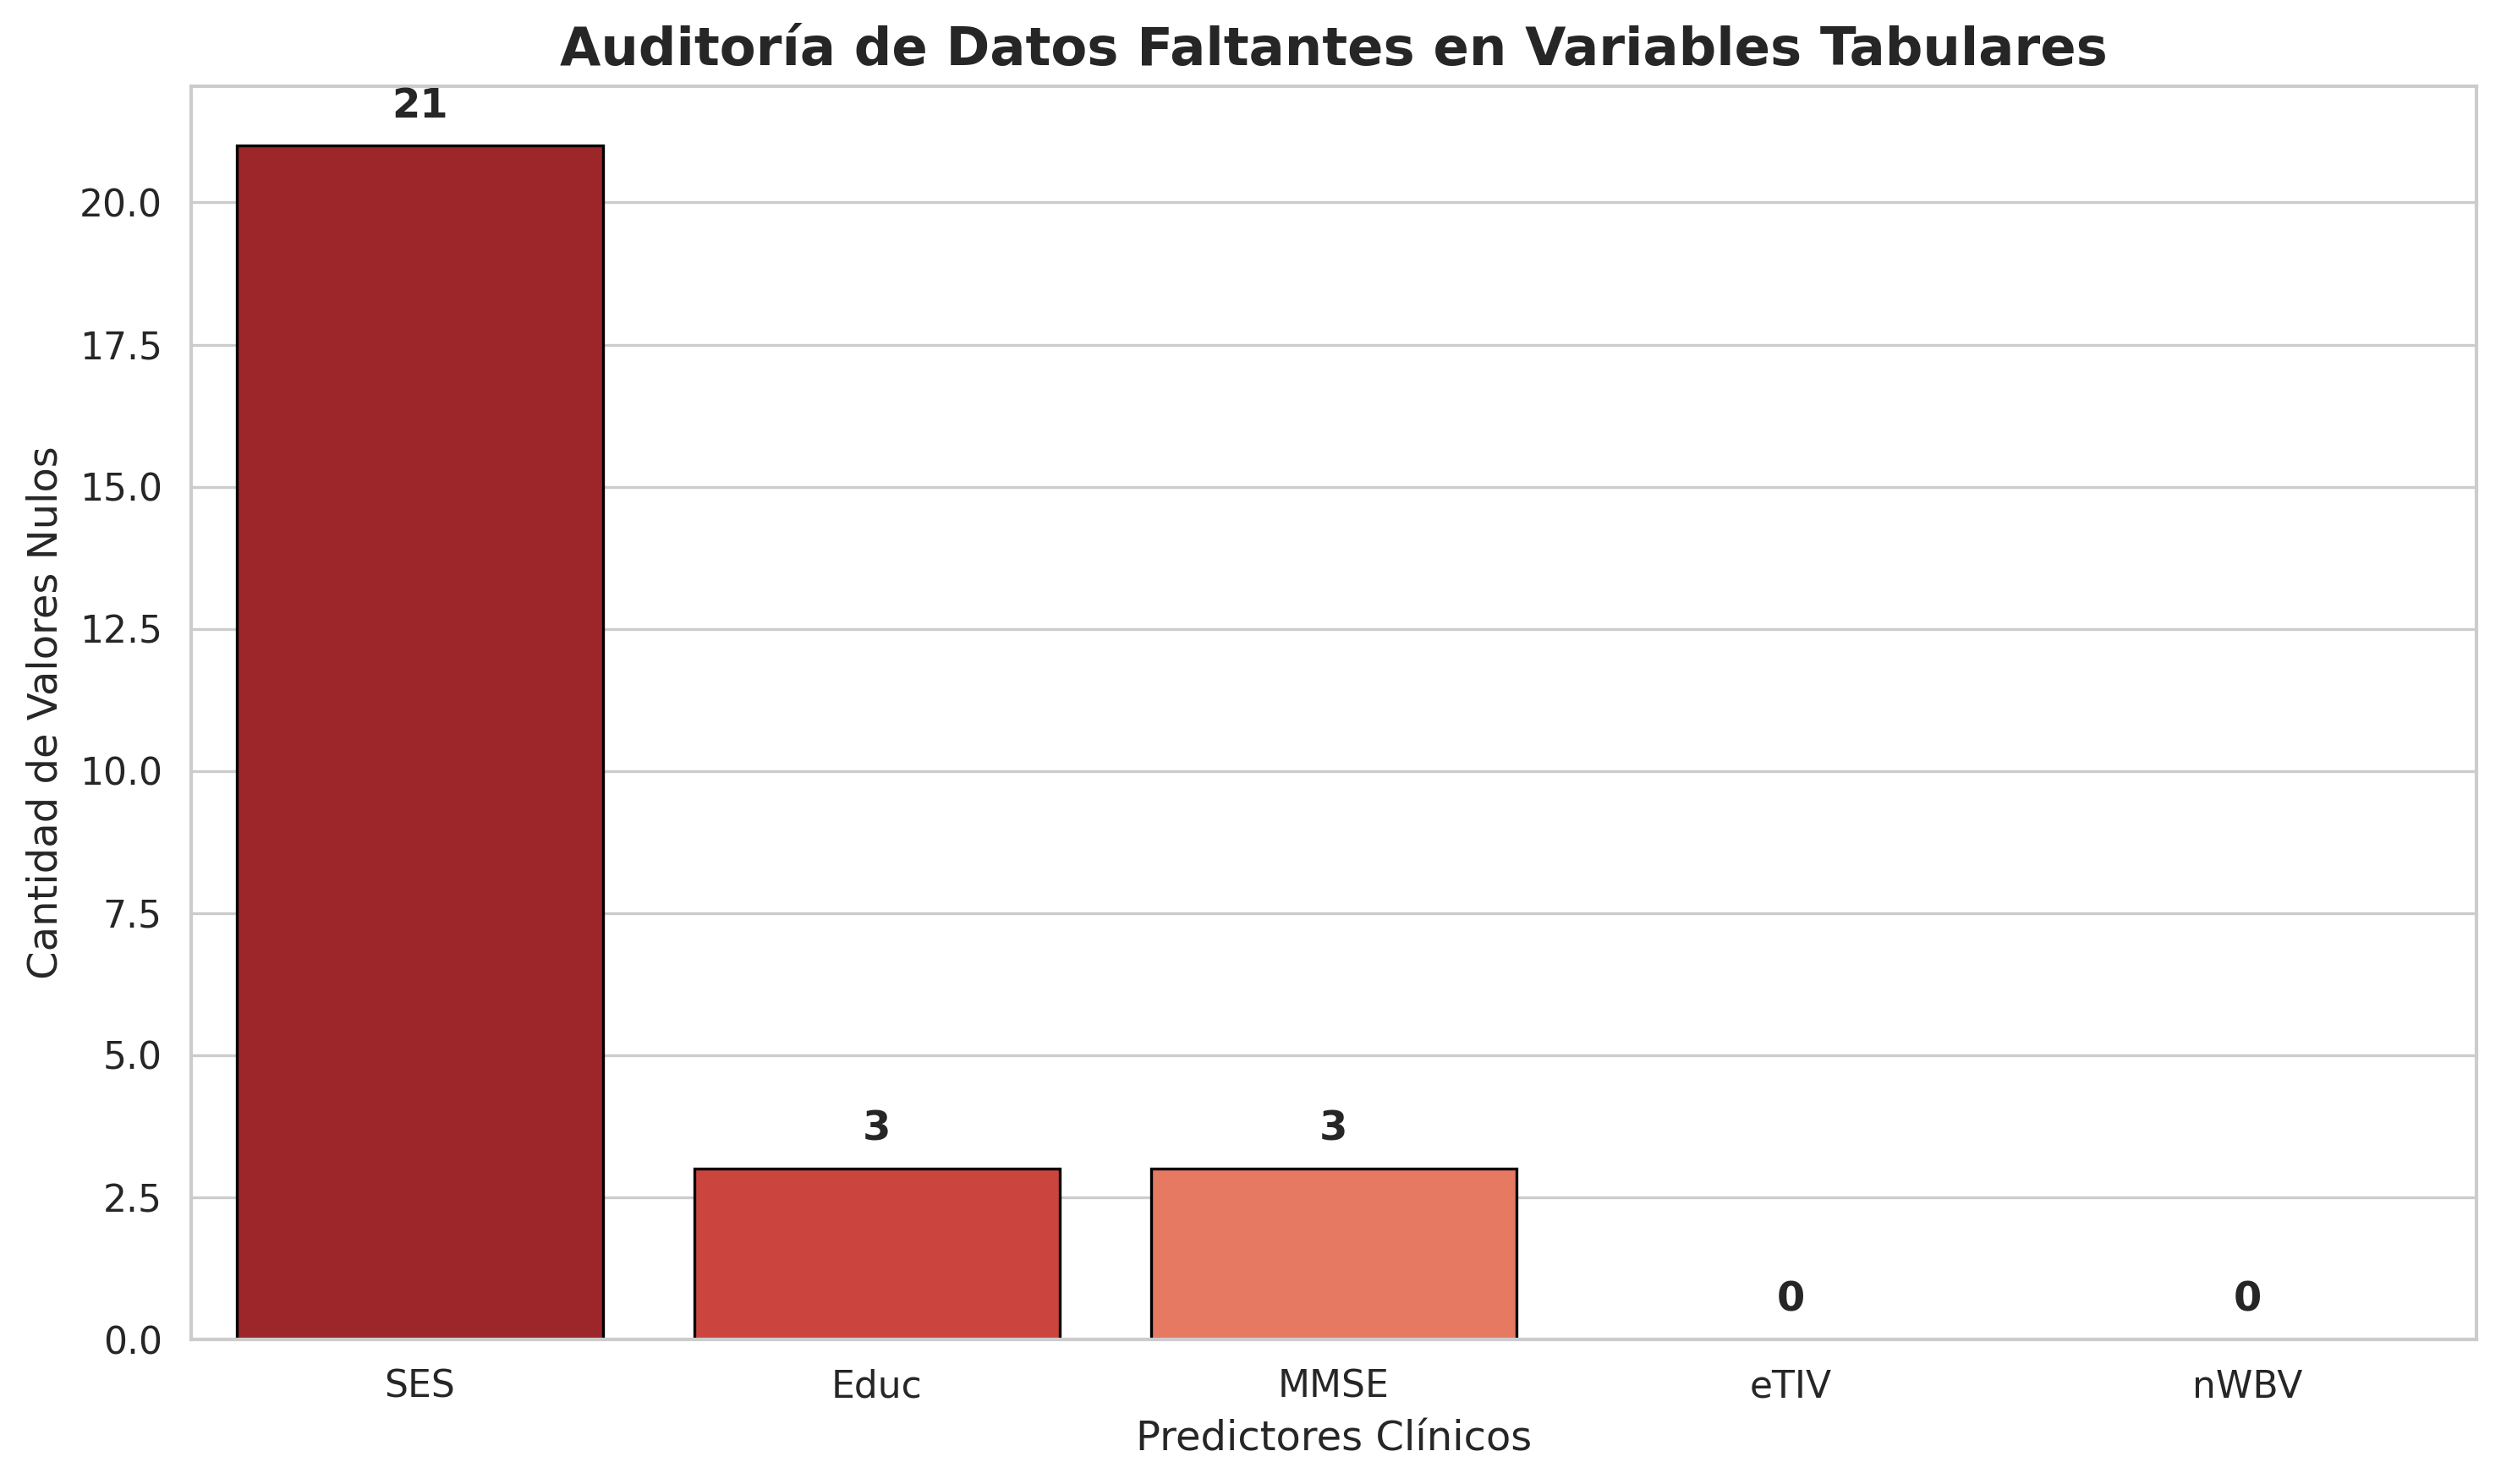
\includegraphics[width=0.85\textwidth]{imagenes/descriptivo/Auditoria_Nulos.png}
	\caption[Revisión de integridad en la cohorte previa al filtrado final]{La robustez de las variables morfométricas permitió centrar las exclusiones en la ausencia crítica de etiquetas diagnósticas o archivos de imagen.}
	\label{fig:auditoria_nulos}
\end{figure}

\subsection{Perfil Demográfico y Distribución Clínica} \label{subsec:perfil_demografico}

La caracterización de la muestra final consolidada ($N=172$) (Tabla \ref{tab:dist_poblacional}) revela un ligero desbalance inicial hacia la clase sana, mientras que el Deterioro Cognitivo Leve (MCI) constituye el segmento intermedio más denso. Cabe destacar que, para el análisis multiclase, se optó por unificar la categoría de demencia moderada (CDR = 2.0) con la de deterioro leve (CDR = 1.0) bajo la etiqueta conjunta de ``Alzheimer/Demencia'', debido a la escasa representatividad de la primera ($N=2$) y con el fin de evitar que el modelo sufriera un sesgo por escasez de muestras en los estadios más avanzados. Estas imágenes preprocesadas y exportadas en formato digital son las que servirán de entrada directa al cuerpo de la red neuronal convolucional.

\begin{table}[htbp]
	\centering
	\caption[Distribución de la cohorte definitiva por estadio clínico y edad.]{Distribución de la cohorte definitiva por estadio clínico (CDR) y franja de edad, calculada exclusivamente sobre los pacientes no descartados en la fase de consolidación. \textbf{Fuente:} elaboración propia.}
	\label{tab:dist_poblacional}
	\resizebox{\textwidth}{!}{%
		\begin{tabular}{lcc|lcccc@{}}
			\toprule
			\textbf{Estadio (CDR)} & \textbf{Pacientes} & \textbf{\%} & \textbf{Franja Edad} & \textbf{Sano} & \textbf{MCI} & \textbf{Alzheimer/Demencia} & \textbf{Total} \\ \midrule
			Sano (0.0) & 91 & 52.9\% & 56-65 años & 18 & 4 & 1 & 23 \\
			MCI (0.5) & 58 & 33.7\% & 66-75 años & 33 & 23 & 7 & 63 \\
			Deterioro (1.0) & 21 & 12.2\% & 76-85 años & 22 & 27 & 10 & 59 \\
			Moderado (2.0) & 2 & 1.2\% & 86+ años & 18 & 4 & 5 & 27 \\ \bottomrule
		\end{tabular}%
	}
\end{table}

Sin embargo, al replantear el problema bajo un enfoque de clasificación binaria (\textbf{Sano vs. Patológico}), el desbalance de clases prácticamente desaparece. Al consolidar todos los estadios de deterioro (CDR 0.5, 1.0 y 2.0) en un único grupo de ``Enfermo'', se obtiene una distribution casi paritaria (Tabla \ref{tab:dist_binaria}). Esta configuración resulta ideal para el descenso de gradiente, ya que permite que la red neuronal aprenda a distinguir patrones morfológicos sin que ninguna clase domine injustificadamente la función de pérdida.

\begin{table}[htbp]
	\centering
	\caption[Distribución binaria de la cohorte para el entrenamiento del clasificador.]{Distribución binaria de la cohorte para el entrenamiento del clasificador. La clase ``Enfermo'' incluye la agregación de los estadios CDR 0.5 y 1.0, así como el colapso de los casos con CDR 2.0. \textbf{Fuente:} elaboración propia.}
	\label{tab:dist_binaria}
	\resizebox{\textwidth}{!}{%
		\begin{tabular}{lcc|lcccc@{}}
			\toprule
			\textbf{Categoría Binaria} & \textbf{Pacientes} & \textbf{\%} & \textbf{Franja Edad} & \textbf{Sano} & \textbf{Enfermo} & \textbf{Total} \\ \midrule
			Sano (CDR 0.0) & 91 & 52.9\% & 56-65 años & 18 & 5 & 23 \\
			Enfermo (CDR $>$ 0) & 81 & 47.1\% & 66-75 años & 33 & 30 & 63 \\
			& & & 76-85 años & 22 & 37 & 59 \\
			\textbf{Total} & \textbf{172} & \textbf{100\%} & 86+ años & 18 & 9 & 27 \\ \bottomrule
		\end{tabular}%
	}
\end{table}

El histograma de la Figura \ref{fig:hist_edades} muestra el solapamiento de poblaciones en la séptima y octava década de vida. Esta paridad numérica en el modelo binario garantiza que el éxito de la clasificación no dependa de la frecuencia de los datos, sino de la capacidad de \textit{ConvNeXt} para detectar las alteraciones estructurales que diferencian ambos grupos.

\begin{figure}[htbp]
	\centering
	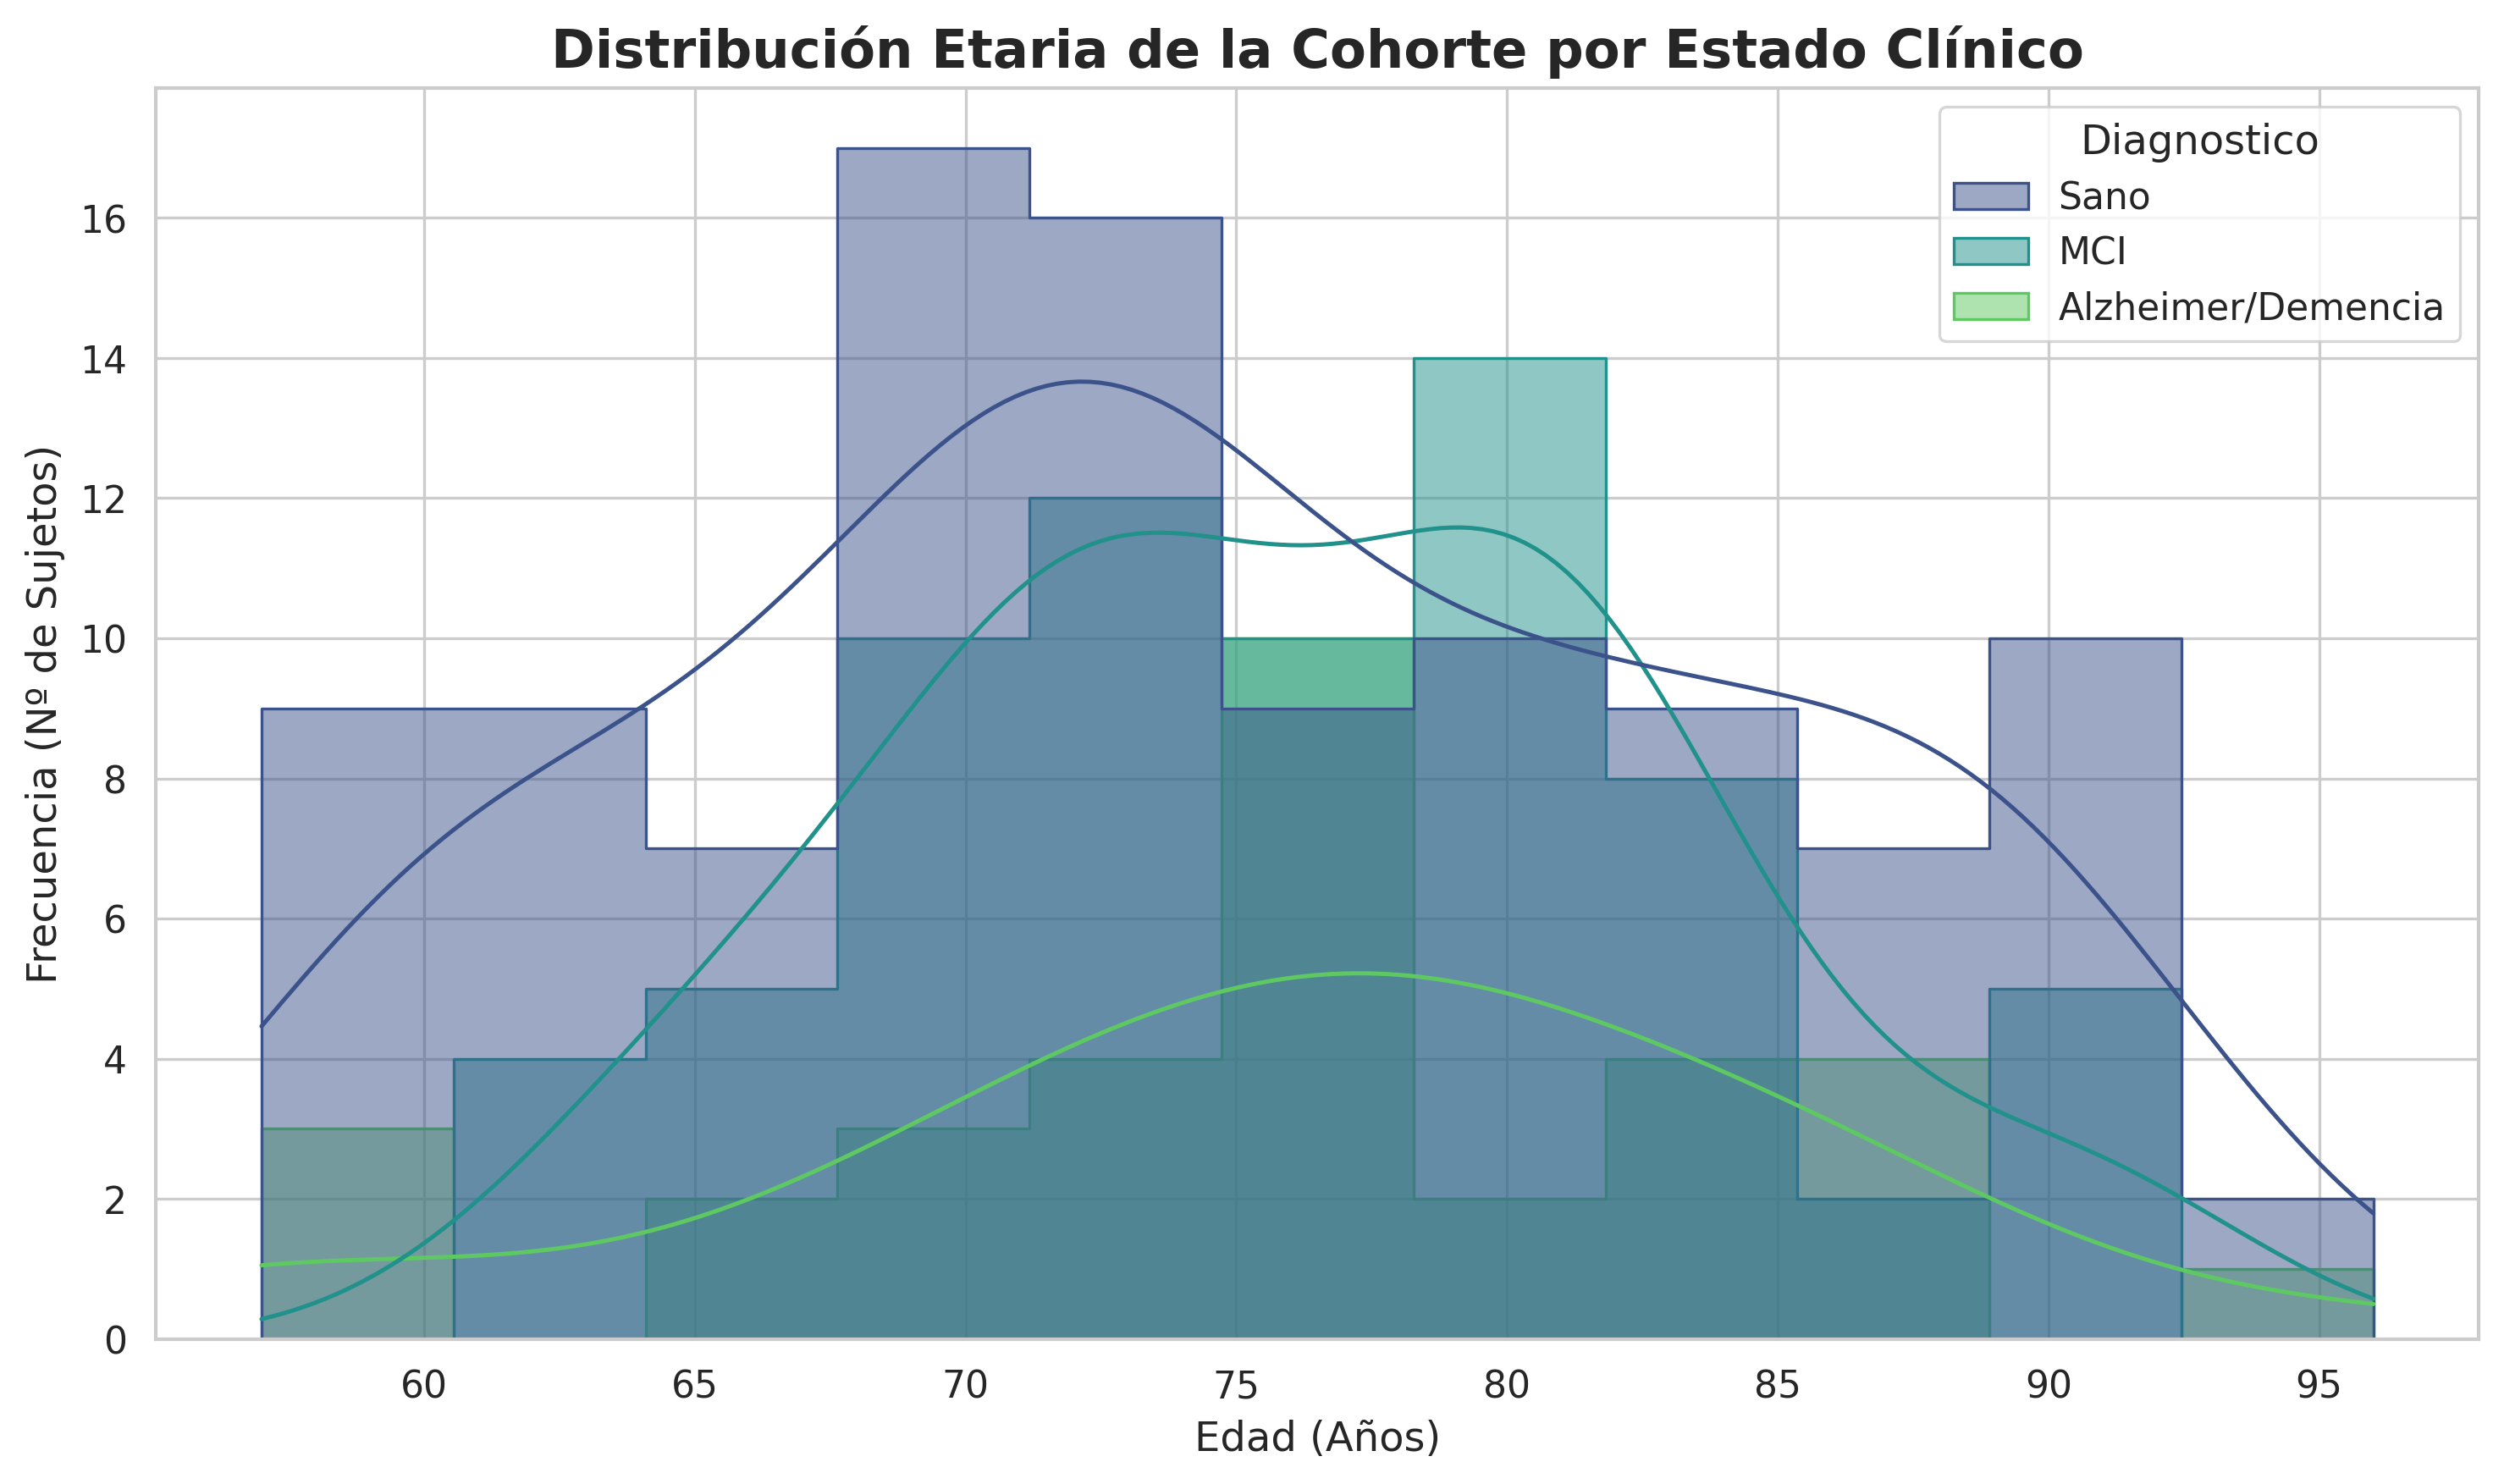
\includegraphics[width=0.85\textwidth]{imagenes/descriptivo/Histograma_Edades.png}
	\caption[Distribución etaria de la cohorte por estado clínico.] {Se aprecia la necesidad de biomarcadores visuales debido al solapamiento de poblaciones en el rango geriátrico.}
	\label{fig:hist_edades}
\end{figure}

\subsection{Análisis de Correlación y Multicolinealidad} \label{subsec:analisis_correlacion}

Para fundamentar el diseño de los escenarios experimentales, se analizó la redundancia entre predictores mediante una matriz de correlación (Figura \ref{fig:matriz_corr}). Dado que el estadio clínico representa una progresión natural de la enfermedad, en este análisis exploratorio preliminar la etiqueta diagnóstica (derivada de la escala CDR) se codificó y trató analíticamente como un factor ordinal. Por este motivo, se aplicó el coeficiente de correlación de Spearman, el cual es idóneo para capturar relaciones monótonas entre variables continuas y categóricas ordenadas. De este análisis se destaca la fuerte correlación negativa del MMSE ($-0.67$) con el diagnóstico, confirmando su papel como indicador clínico de referencia. Asimismo, el análisis reveló una correlación perfecta determinista ($r = -1$) entre el volumen intracraneal (eTIV) y el factor de escala del atlas (ASF). Al ser variables linealmente dependientes, se decidió excluir la variable ASF.

\begin{figure}[htpb]
	\centering
	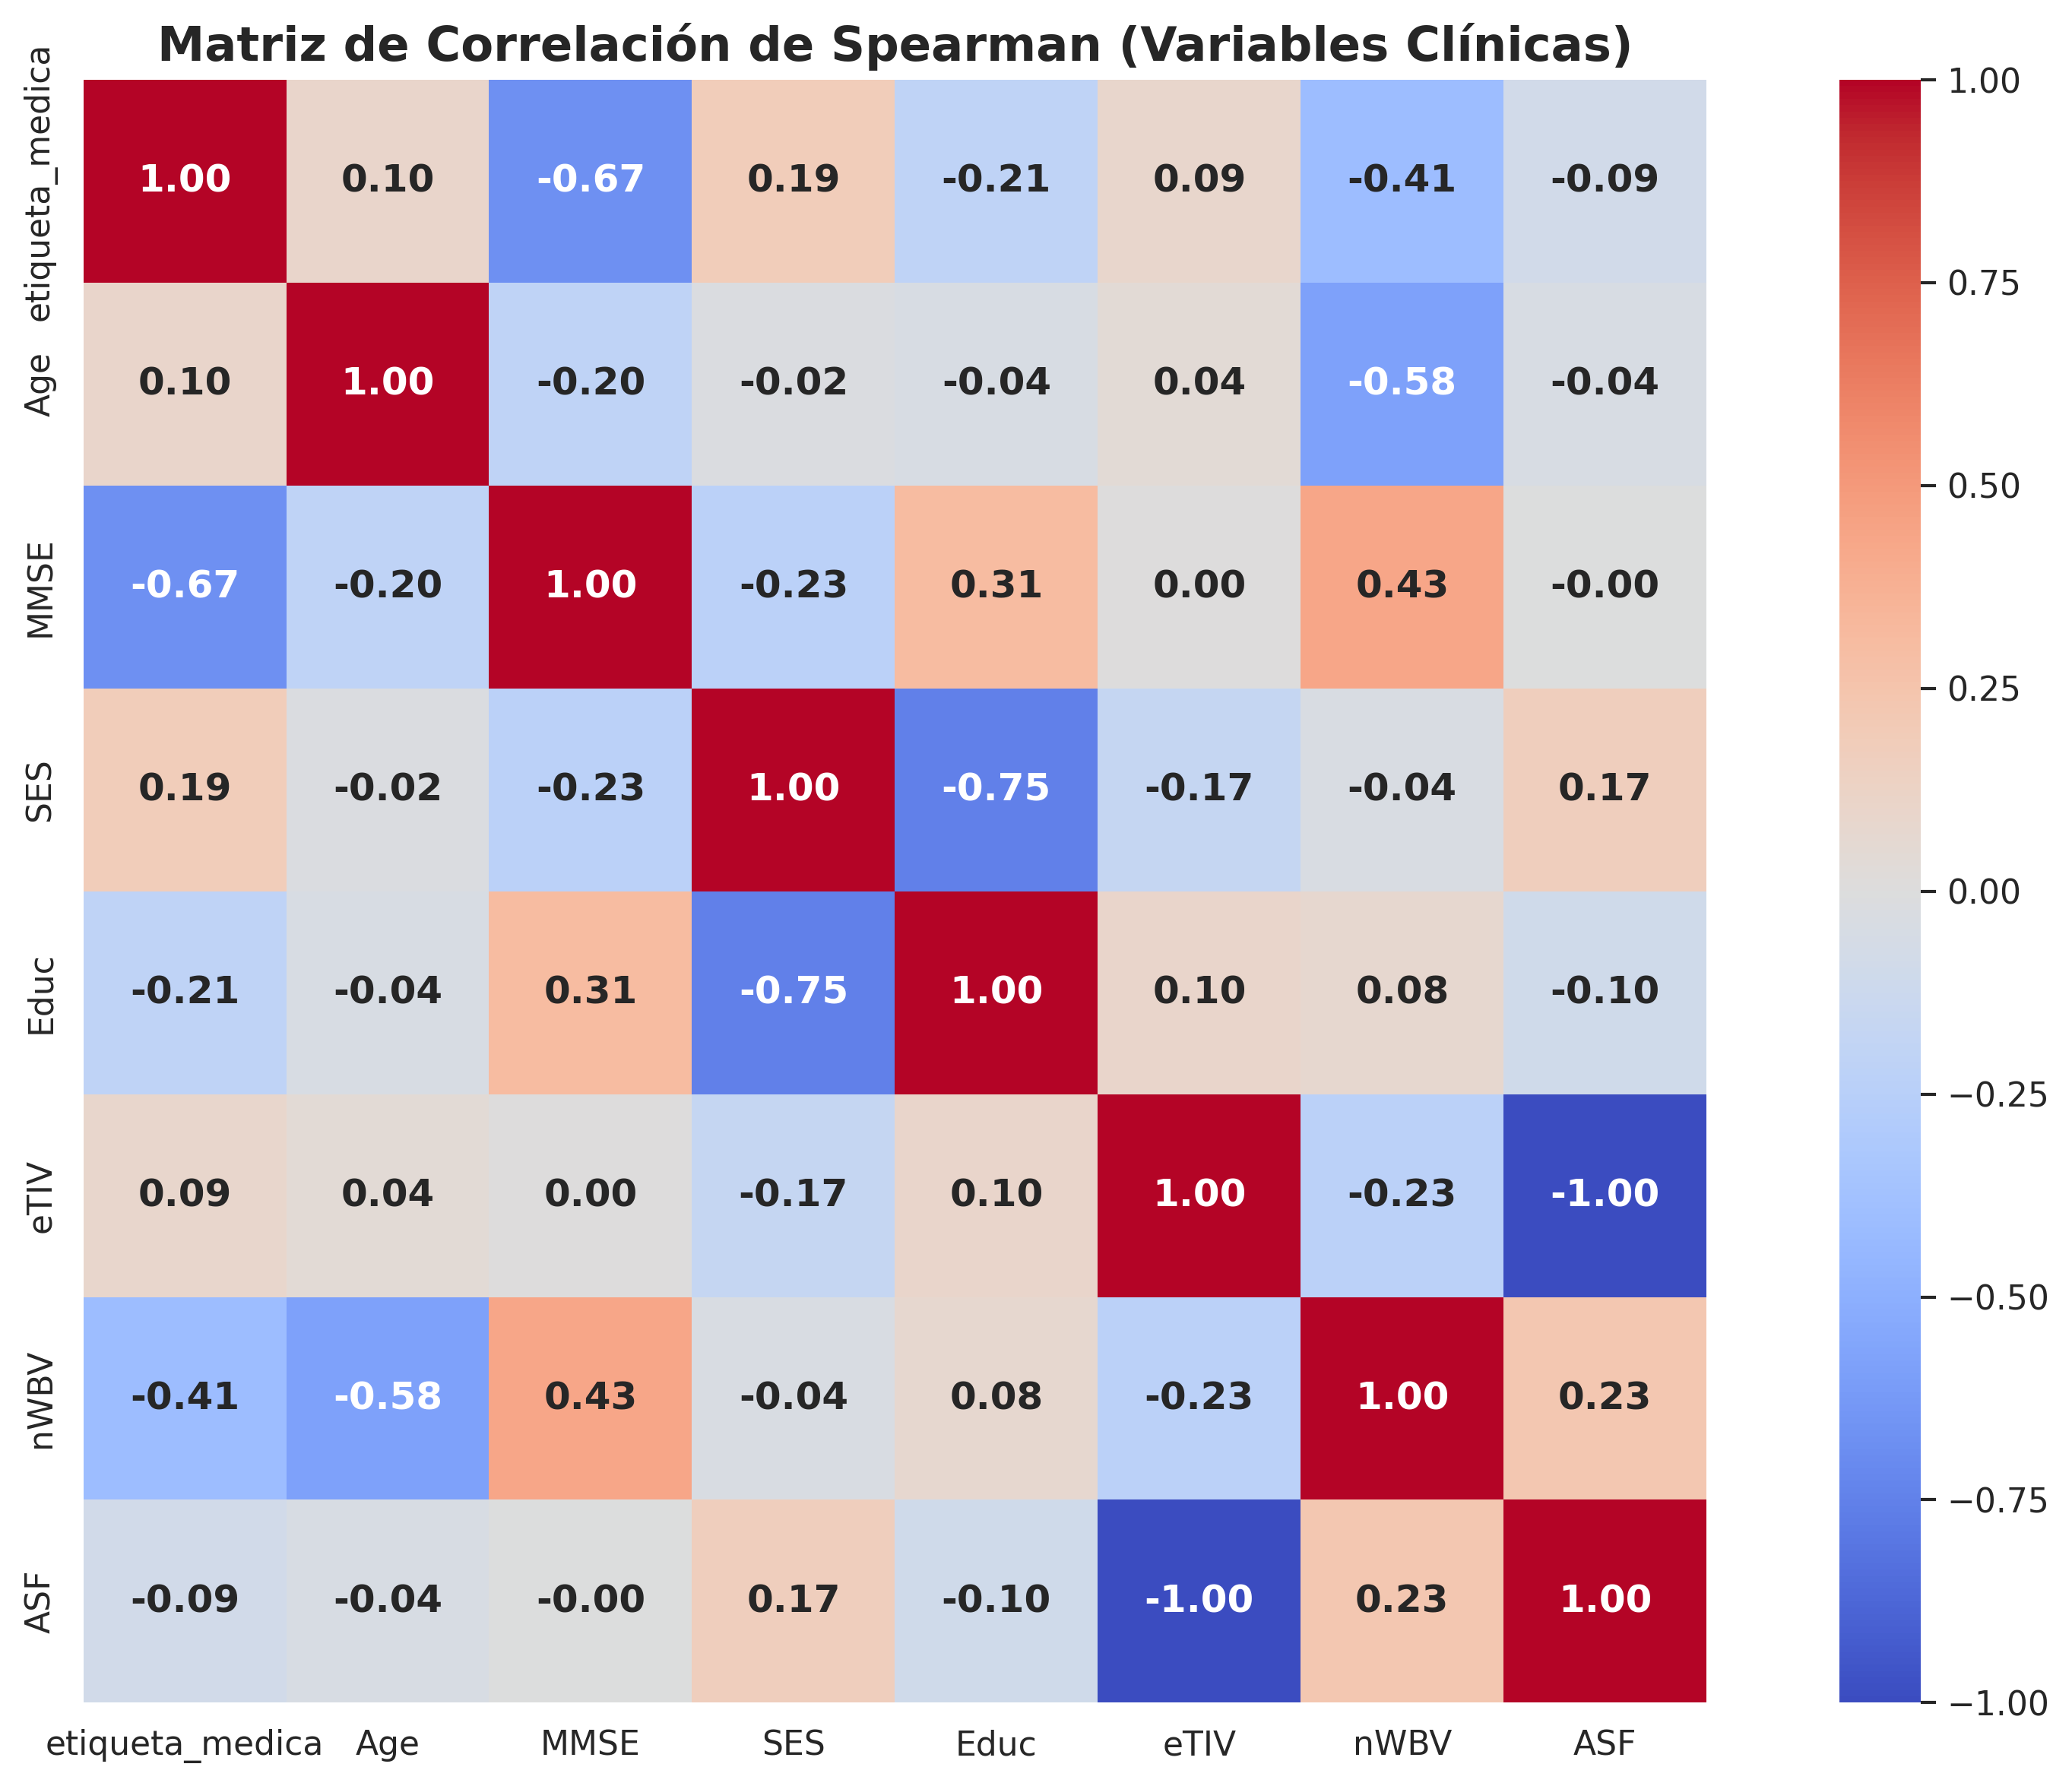
\includegraphics[width=0.85\textwidth]{imagenes/descriptivo/05_Matriz_Correlacion.png}
	\caption[Matriz de correlación de Spearman] {Matriz de correlación de Spearman. Los coeficientes validan la jerarquía de importancia de las variables MMSE y nWBV sobre el diagnóstico final. \textbf{Fuente:} elaboración propia.}
	\label{fig:matriz_corr}
\end{figure}

Establecida esta configuración de los predictores, la representación matemática de esta etiqueta diagnóstica se adaptó de forma específica según el tipo de experimento. En el \textbf{enfoque binario}, la variable objetivo se transformó en una variable booleana ($0$ o $1$), ya que las funciones de pérdida en \textit{PyTorch} necesitan trabajar obligatoriamente con tensores de tipo entero o punto flotante para poder evaluar la función de coste y guiar el descenso de gradiente sobre la red \textit{ConvNeXt}. Por otro lado, en el \textbf{enfoque ordinal multiclase}, la variable objetivo mantiene la naturaleza de un factor ordenado mediante la definición de tres clases secuenciales ($0, 1, 2$). Cabe recordar que estas tres clases aglutinan los cuatro estadios originales de la escala CDR debido a la reagrupación del nivel de demencia grave ($CDR = 2.0$) dentro de la categoría moderada ($CDR = 1.0$), por la extrema escasez de muestras en el grado más avanzado de la patología y con el fin de no perder la información de dichos pacientes. En lugar de procesar estas tres etiquetas como categorías independientes donde se ignoraría la distancia entre las distintas fases, se implementó la arquitectura CORAL (cuyos fundamentos teóricos se detallan en la Sección \ref{subsec:ordinal_coral_teoria}). 


Finalmente, la cohorte queda consolidada en una muestra de 172 pacientes libre de variables de confusión. El proceso de tratado y limpieza de datos aplicado sobre las imágenes ha permitido transformar los escaneos y metadatos en bruto en una base de entrenamiento sólida y metodológicamente honesta. Estructurar el origen de estas fuentes, clasificar las variables demográficas, psicométricas y morfométricas que describen a cada sujeto, y dar paso a un análisis exploratorio riguroso, han sido etapas fundamentales para asentar el proyecto. Pasos como el filtrado demográfico a partir de los 56 años para neutralizar el sesgo de edad, el estudio del perfil demográfico y su distribución clínica para balancear los grupos, y el análisis de correlación, constituyen decisiones críticas para asegurar que el modelo identifique la atrofia neurodegenerativa real, impidiendo que tome atajos estadísticos. Una vez garantizada la calidad de los datos de entrada, dejamos atrás la exploración de los datos para centrarnos en el marco metodológico del proyecto, dando paso al siguiente capítulo, donde abordaremos el diseño de la arquitectura de visión artificial, las reglas de validación cruzada y las estrategias de fusión multimodal.

\chapter{Marco Metodológico y Diseño Experimental} \label{chap:metodologia}

Este capítulo detalla, paso a paso, las decisiones metodológicas que dan forma a nuestro modelo predictivo. Dado el tamaño reducido de la muestra ($N = 172$), el diseño experimental prioriza la protección frente al sobreajuste. Para ello, los modelos se basan en un particionamiento estricto de partición por paciente y una estratificación dual diseñada para evitar sesgos por envejecimiento natural.

Sobre esta base de validación, se describe el núcleo del extractor visual: una red neuronal adaptada para procesar secuencias de resonancias (enfoque 2.5D) que preserva los detalles de la atrofia y aprende a centrar su atención en los planos anatómicos más relevantes. A continuación, se expone cómo el sistema evoluciona desde una tarea de cribado binario (Sano frente a Patológico) hasta un modelo capaz de predecir la progresión continua de la enfermedad (Sano $\rightarrow$ MCI $\rightarrow$ Demencia). Finalmente, se detalla la estrategia de integración multimodal, encargada de cruzar de forma inteligente lo que la red ha detectado en la imagen con el perfil cognitivo del paciente. A través de este recorrido, se demostrará cómo cada decisión ha sido tomada para maximizar la generalización del modelo y garantizar un dictamen médico equilibrado, interpretable y estadísticamente estable.

% =========================================================
% SECCIÓN 4.1: PROTOCOLO DE INTEGRIDAD DE LA VALIDACIÓN
% =========================================================


\section{Diseño de Escenarios Experimentales y Gestión de Variables} \label{sec:diseno_escenarios}

Para evaluar el impacto de cada tipo de información y garantizar el rigor de los modelos, se ha definido una estrategia experimental basada en una integración progresiva de complejidad. Este diseño permite realizar una comparación directa entre las predicciones extraídas por el algoritmo visual y los marcadores médicos tradicionales, evaluando su comportamiento tanto de forma aislada como en esquemas de orquestación multimodal.

\begin{itemize}
	
	\item \textbf{Gestión de Variables y Referencia}:
	
	\begin{itemize}
		
		\item \textit{Referencia de Diagnóstico (CDR)}: Se excluye como variable de entrada, utilizándose exclusivamente como variable objetivo para supervisar el entrenamiento y validar las predicciones.
		
		\item \textit{Variables de Control (Edad, EDUC, SES, eTIV)}: Se mantienen constantes en todos los entornos tabulares y de fusión para situar cada anatomía en su contexto demográfico y biológico individual.
		
	\end{itemize}
	
\end{itemize}

Para cuantificar el beneficio real de la neuroimagen y detectar posibles problemas de dominancia (véase en la Sección \ref{subsec:sota_colapso_multimodal}), se han establecido los siguientes niveles de experimentación. Cabe destacar que, aunque el sistema procesa internamente un modelo tabular basado exclusivamente en las variables demográficas para tomarlo como base de una fusión multimodal simple, este modelo aislado carece de la relevancia predictiva y contundencia clínica necesarias para el diagnóstico por sí solo. Por lo tanto, su única función es estrictamente estructural dentro del ensamblaje, y no será mostrado ni tenido en cuenta de forma independiente en la evaluación de resultados.

El esquema de experimentación se estructura en los siguientes niveles de complejidad, correspondientes a los modelos definitivos de la investigación:

\begin{enumerate}
	\item \textbf{Evaluación Aislada (Ramas Unimodales)}:
	\begin{itemize}
		\item \textit{Rama Visual Aislada}: Emplea exclusivamente la neuroimagen como entrada, omitiendo cualquier metadato. Sirve como línea base para evaluar la capacidad intrínseca de la red \textit{ConvNeXt} en la detección de patrones de atrofia sin ningún contexto externo.
		\item \textit{Ramas Tabulares Clínicas}: Integran el perfil demográfico junto a los biomarcadores médicos. Se evalúan dos variantes para actuar como estándar clínico comparativo: un modelo sin test cognitivo, añadiendo solo la volumetría \textit{nWBV} (\textit{normalized Whole Brain Volume}) y un modelo completo (incorporando además el test psicométrico \textit{MMSE}).
	\end{itemize}
	
	\item \textbf{Orquestación Multimodal (Fusión Visual-Tabular)}:
	\begin{itemize}
		\item \textit{Fusión Base}: Integra la neuroimagen exclusivamente con las variables demográficas de control. Mide la eficacia de la arquitectura para identificar patrones patológicos apoyándose en el perfil sociodemográfico del paciente, sin la intervención de evaluaciones médicas previas.
		\item \textit{Fusión Sin MMSE}: Incorpora la variable \textit{nWBV} a la fusión base. Actúa como un test de calidad sobre la extracción de características: si el rendimiento no presenta un incremento significativo, se demuestra que la red ha aprendido a computar la información volumétrica por sí misma.
		\item \textit{Fusión Completa}: Incluye la totalidad de las variables, incorporando el test \textit{MMSE}. Es el escenario crítico para analizar el sesgo de modalidad (\textit{Modality Laziness}) y evaluar si la visión artificial logra un incremento predictivo complementario (capacidad de rescate) en pacientes donde la evaluación clínica tradicional no arroja resultados concluyentes.
	\end{itemize}
\end{enumerate}

\section{Integridad de la Validación: Particionado y Estratificación Dual} \label{sec:integridad_validacion}

Para garantizar la capacidad de generalización del sistema y evitar sesgos de evaluación frecuentes en este ámbito, como los comentados en la Sección \ref{subsec:sota_reproducibilidad}, se ha implementado un marco de validación estricto. Esta configuración asegura que las inferencias del modelo se basen exclusivamente en patrones reales de la patología, tanto a nivel visual como con los datos tabulares, y no en sesgos derivados del diseño experimental o la distribución de la muestra.

Como defensa primaria, se impuso una \textbf{partición estricta a nivel de sujeto} (\textit{Subject-Level Split}). Siguiendo los fundamentos de la Sección \ref{subsec:integridad_leakage}, este criterio garantiza que la totalidad de los datos de un paciente (incluyendo todos sus cortes transversales y metadatos) se asignen de forma excluyente a un único conjunto. Al evitar el paradigma de \textit{Slice-Level Split}, se anula el riesgo de que la arquitectura \textit{ConvNeXt} memorice rasgos anatómicos individuales o ruido específico del sensor, obligando al optimizador a extraer patrones de neurodegeneración aplicables a nuevas anatomías no vistas anteriormente.

Complementariamente, para mitigar el desplazamiento de la covariable (\textit{Covariate Shift}) por edad detallado en la Sección \ref{subsec:covariate_shift_teoria}, se desarrolló e implementó una técnica de \textbf{Estratificación Dual}. Esta solución surgió como una idea propia, cuyo alcance técnico se potenció con la asistencia de herramientas de inteligencia artificial (en línea con lo expuesto en la Sección \ref{subsec:ia_codiseno}). Esta herramienta permitió consolidar la propuesta y darle forma, además de proporcionar las bases bibliográficas necesarias para corroborar su validez, fundamentando la estrategia en el trabajo de Sechidis et al. \cite{sechidis2011}. Este estudio demuestra empíricamente que agrupar combinaciones de variables en una sola etiqueta compuesta es la forma matemáticamente óptima de preservar la distribución conjunta original a lo largo de todos los subconjuntos.

En la práctica, se segmentó la muestra en cuartiles de edad ($\text{Age\_Quartile}$) para generar esta variable sintética mediante el producto cartesiano con el diagnóstico clínico (CDR):

\begin{equation}
	\text{Strat\_Dual}_i = \text{Etiqueta}_i \times \text{Age\_Quartile}_i
\end{equation}

Al equilibrar conjuntamente la edad y la gravedad de la enfermedad en cada pliegue de la validación cruzada, se consiguen dos grandes beneficios. En primer lugar, se bloquea el sesgo de confusión: dado que el envejecimiento natural también reduce el volumen cerebral, esta técnica impide que un grupo de prueba concentre por azar a los pacientes mayores, evitando que la red aprenda a predecir la edad en lugar del Alzheimer. En segundo lugar, al trabajar con una muestra tan reducida ($N=172$), un particionamiento simple induciría una alta varianza estocástica. Dado el bajo ratio de combinaciones posibles en nuestra cohorte (12 agrupaciones frente al total de pacientes), la técnica aplicada minimiza dicha varianza y asegura la estabilidad del experimento, tal y como certifican Sechidis et al. De este modo, se garantiza que el hiperplano de decisión se evalúe siempre sobre una distribución idéntica, evitando que un potencial rendimiento alto del modelo sea fruto de una casualidad estadística y forzando al algoritmo a centrarse únicamente en la atrofia patológica real.


\section{Arquitectura Visual 2.5D: Aprendizaje en Datos Reducidos} \label{sec:arquitectura_visual_diseno}

Para procesar la complejidad de la resonancia magnética eludiendo el coste computacional de las redes 3D, se ha diseñado la arquitectura \textit{HybridAgile\_MIDL}. Siguiendo el paradigma 2.5D fundamentado en la Sección \ref{subsec:paradigma_25d_teoria}, el modelo opera sobre una entrada de 16 cortes transversales integrados como canales de información.

Esta configuración responde a un compromiso entre fidelidad anatómica y restricciones de hardware (Sección \ref{subsec:hardware_kaggle}). La adopción del régimen 2.5D permite maximizar la resolución de entrada y la profundidad de la red en GPUs más limitadas, garantizando la estabilidad del gradiente incluso ante la escasez muestral de la cohorte OASIS-1 ($N = 172$). El flujo completo de ambos enfoques se ilustran en la Figura \ref{fig:red_binaria} para el escenario binario y en la Figura \ref{fig:red_multiclase_coral} para el multiclase ordinal.

\begin{figure}[htbp]
	\centering
	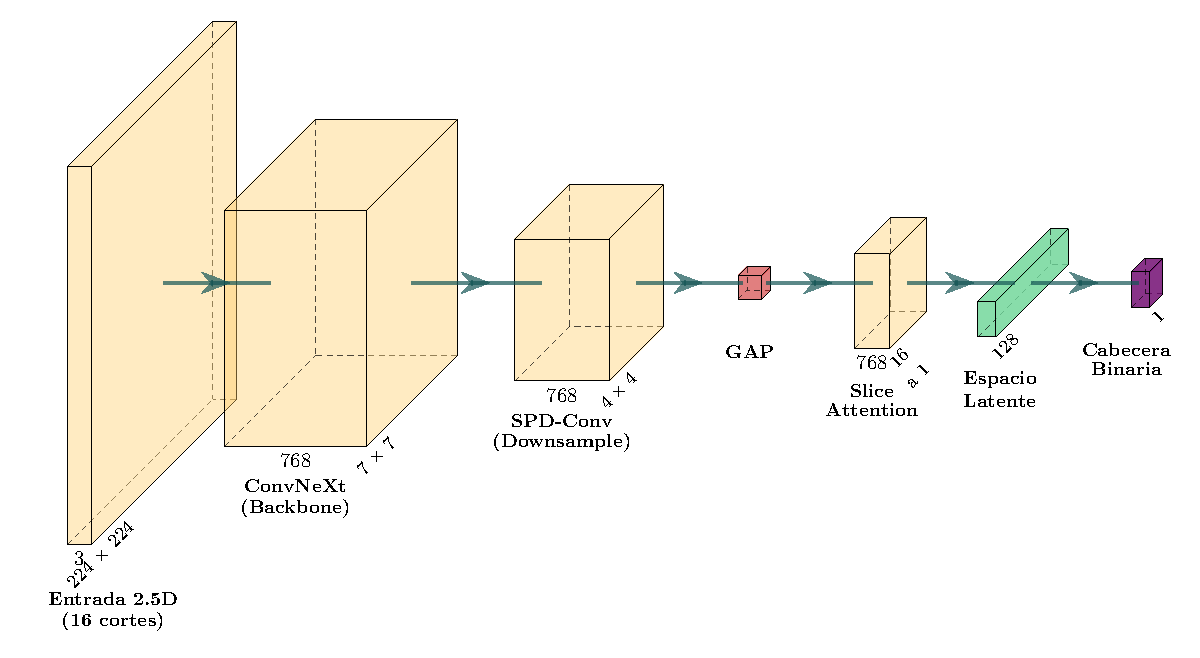
\includegraphics[width=\textwidth]{red_binaria.pdf}
	\caption[Arquitectura visual 2.5D propuesta]{Arquitectura visual 2.5D propuesta. Se detalla el flujo desde la entrada multisección hasta la cabecera de decisión binaria. \textbf{Fuente:} elaboración propia.}
	\label{fig:red_binaria}
\end{figure}

\begin{figure}[htbp]
	\centering
	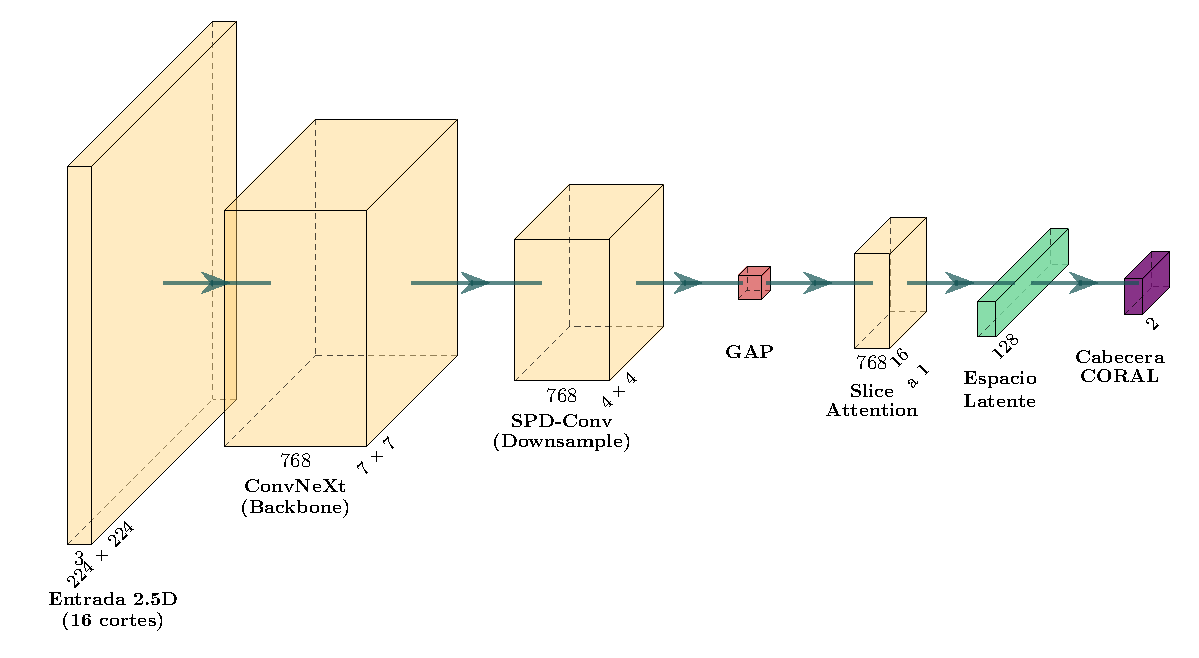
\includegraphics[width=\textwidth]{red_multiclase.pdf}
	\caption[Arquitectura multiclase con cabecera CORAL]{Arquitectura multiclase con cabecera CORAL. Se observa la proyección del espacio latente sobre los nodos de salida para modelar la jerarquía de la patología. \textbf{Fuente:} elaboración propia.}
	\label{fig:red_multiclase_coral}
\end{figure}

\subsection{Backbone Visual y Adaptación SPD-Conv} \label{subsec:diseno_backbone_spd}

Como motor de extracción de características se ha seleccionado una red \textit{ConvNeXt-Tiny} preentrenada (Sección \ref{subsec:cnn_convnext}). Para adaptar esta arquitectura al escenario de \textit{Small Data}, se han aplicado dos modificaciones estructurales clave:

\begin{enumerate}
	\item \textbf{Preservación de Granularidad}. Se sustituyó la capa de reducción inicial por un módulo \textbf{SPD-Conv} con un factor de bloque de 2 (Sección \ref{subsec:spd_conv_teoria}). Al reordenar los píxeles hacia los canales en lugar de eliminarlos, la red retiene la densidad de la sustancia gris y la morfología del hipocampo, elementos que a menudo se degradan en las convoluciones que utilizan un paso extendido o \textit{stride} estándar (cuyos conceptos base se definieron en la Sección \ref{subsec:cnn_convnext}) \cite{sikiric2022no}.
	
	\item \textbf{Estrategia de Congelación Bifurcada}. La retención de pesos se adaptó específicamente a la complejidad de cada tarea para garantizar la estabilidad del gradiente.
	\begin{itemize}
		\item \textit{Régimen Binario (Congelación Parcial)}: Se bloquearon exclusivamente los bloques residuales inferiores. Esto permite que actúen como extractores de rasgos genéricos, mientras que las capas superiores mantienen capacidad de aprendizaje para define de forma precisa la separación entre el tejido sano y el patológico.
		
		\item \textit{Régimen Ordinal (Deep Freezing)}: A diferencia del enfoque binario, en el modelo de progresión clínica se impuso una congelación total de los pesos del \textit{backbone} \cite{liu2022convnet}. Al tratar con una clasificación ordinal sobre una muestra reducida ($N = 172$), permitir que la red modifique sus filtros genéricos induciría un sobreajuste drástico hacia las características únicas de los escasos pacientes con demencia severa. Así, el cuerpo convolucional queda blindado, actuando como un extractor anatómico fijo que delega todo el esfuerzo de optimización al mecanismo de atención y a la cabecera CORAL.
	\end{itemize}
\end{enumerate}

\subsection{Mecanismo de Atención Inter-Corte (Slice-Attention)} \label{subsec:diseno_slice_attention}

Dado que la atrofia no es uniforme en todo el volumen tridimensional, el modelo incorpora un módulo de \textbf{Slice-Attention} enfocado en calcular un vector de coeficientes dinámicos (pesos de atención) para ponderar la relevancia de cada uno de los 16 planos transversales de entrada (véase la Sección \ref{subsec:atencion_teoria}). Este planteamiento nació como una propuesta propia a partir de la observación clínica: determinados cortes centrales albergan marcadores críticos del Alzheimer (como el volumen del hipocampo), mientras que otros, debido a su ubicación periférica, apenas contienen información diagnóstica relevante. 

La asignación y el cálculo de estos coeficientes de importancia inter-corte se gestiona de manera directa mediante la función de activación híbrida \textbf{MAF} (Sección \ref{subsec:maf_teoria}), que combina ReLU, SiLU y GeLU para suavizar la respuesta del mecanismo de atención. Esta ponderación no lineal permite que el sistema identifique de forma automática las secciones con mayor dilatación de los ventrículos o encogimiento del tejido cerebral (cuya relevancia biológica como marcadores de la enfermedad se detalló en la Sección \ref{sec:bases_biologicas_alzheimer}), atenuando el impacto de los cortes secundarios periféricos y optimizando la extracción de características globales.

Para materializar esta intuición clínica en una arquitectura funcional, se emplearon herramientas de inteligencia artificial como asistentes de desarrollo técnico y estructuración (conforme a la declaración de uso de la Sección \ref{subsec:ia_codiseno}). El uso de esta tecnología ayudó a potenciar el diseño original, apoyando la traducción de la idea a código y facilitando bibliografía para revisar el concepto. Bajo el criterio y supervisión final del autor, la estrategia se fundamentó metodológicamente en el marco de atención para múltiples instancias (\textit{Attention-based Multiple Instance Learning}) introducido por Ilse et al. \cite{ilse2018attention}. De este modo, se aseguró que la asistencia de la inteligencia artificial actuara como una herramienta para llevar el trabajo más allá, y en ningún caso como sustituto del rigor analítico.

\subsection{Estrategia de Entrenamiento y Dinámica de Aprendizaje} \label{subsec:estrategia_entrenamiento}

Para garantizar la convergencia en un entorno de datos reducidos, se diseñó una metodología de entrenamiento basado en dos modelos, que ajusta tanto la función de coste como la actualización de pesos según la naturaleza de la tarea. No obstante, ambos enfoques de clasificación (binaria dicotómica y multiclase de factor ordenado) comparten una misma base de diseño computacional: la división de la red en dos bloques diferenciados con ritmos de aprendizaje independientes, compuestos por el tronco convolucional extractor de características y la cabecera de clasificación o módulo de decisión final.

El tronco o \textit{backbone} conforma el núcleo principal de ConvNeXt, encargado de procesar la señal espacial de las resonancias magnéticas para codificar descriptores anatómicos complejos. Por su parte, la cabecera o \textit{head} constituye la etapa de salida que mapea estas representaciones latentes hacia las etiquetas diagnósticas de la patología. En regímenes de \textit{Small Data}, la aplicación de una tasa de aprendizaje única y uniforme para todo este grafo resulta desaconsejable, ya que las actualizaciones drásticas del gradiente tienden a degradar las características jerárquicas previamente consolidadas en ImageNet \cite{liu2022convnet}. Partiendo de esta división estructural común, la estrategia de optimización se especializa para cada escenario experimental:

\begin{itemize}
	\item \textbf{Régimen Binario (Detección y Tasas Diferenciales)}: 
	Se empleó una combinación de \textit{Focal Loss} y \textit{Label Smoothing} para forzar a la red a discriminar anatomías fronterizas, reduciendo la sobreconfianza en las clases mayoritarias. Para optimizar el ajuste, este modelo implementa una estrategia de \textbf{Tasas de Aprendizaje Diferenciales} (\textit{Differential Learning Rates}). Al asignar una tasa de aprendizaje más alta y flexible a la cabecera, se favorece una rápida especialización en las fronteras de decisión de la enfermedad de Alzheimer. En paralelo, mantener una tasa significativamente más baja y conservadora en el tronco convolucional protege los filtros geométricos de bajo nivel (como bordes y contrastes), garantizando un equilibrio óptimo entre la transferencia de conocimiento y la estabilidad del entrenamiento.
	
	\item \textbf{Régimen Ordinal (Progresión sobre Factores Ordenados y Deep Freezing)}: 
	Dada la inestabilidad intrínseca de evaluar la evolución del Alzheimer y la escasez de muestras patológicas, se aplicaron dos medidas de blindaje en el clasificador basado en la cabecera CORAL (\textit{Consistent Rank Logits}), cuyos fundamentos teóricos se detallaron en la Sección \ref{subsec:ordinal_coral_teoria}. 
	
	Cabe recordar que esta arquitectura justifica el tratamiento de la escala clínica CDR como un \textbf{factor ordenado} y no como una variable numérica continua. Esto evita el error estadístico de asumir que las distancias biológicas entre los estadios de deterioro (v.g., de sano a leve frente a de moderado a severo) son lineales y equidistantes. Bajo este esquema jerárquico, la estrategia de optimización se adaptó mediante dos medidas específicas para mitigar el riesgo de sobreajuste:
	
	\begin{enumerate}
		\item \textbf{Deep Freezing Total}: A diferencia del enfoque bimodal del modelo binario, la tasa de aprendizaje efectiva del cuerpo visual se redujo estrictamente a cero mediante la desactivación del cálculo de gradientes (\textit{requires\_grad = False}). Al bloquear por completo la actualización de los pesos del \textit{backbone}, el sistema opera como un extractor de rasgos visuales estático, concentrando todo el esfuerzo de optimización exclusivamente en la cabecera de atención y en los umbrales CORAL para mitigar el riesgo de sobreajuste ante la alta asimetría de las clases.
		\item \textbf{Aprendizaje Sensible al Coste}: Se implementó una pérdida de entropía binaria ponderada por un vector de pesos asimétricos $W = [3.0, 4.5]$. 
	\end{enumerate}
\end{itemize}

Respecto a este último punto, la configuración del vector de penalizaciones responde a dos objetivos clínicos y metodológicos fundamentales:

\textbf{Compensación de la Escasez}. Al subdividirse la clasificación ordinal de tres clases en dos fronteras binarias independientes, cada elemento del vector $W = [3.0, 4.5]$ actúa como el factor de ponderación para la clase positiva ($w_j$) en su respectivo hiperplano de decisión. El primer peso ($w_1 = 3.0$) calibra la frontera inicial (Sano frente a la presencia de cualquier grado de deterioro), contrarrestando el desbalance general del dataset. El segundo peso ($w_2 = 4.5$) se aplica de forma exclusiva a la frontera de demencia avanzada (estadios moderados/severos frente al resto). Dado que esta última clase es la más minoritaria y crítica de la muestra, escalar el gradiente por un factor de $4.5$ inyecta la fuerza suficiente en la retropropagación para que el optimizador extraiga descriptores de atrofia severa sin ser eclipsado por la norma de los ejemplos sanos.

\textbf{Priorización de la Sensibilidad Clínica}. Adicionalmente, esta asimetría en los pesos penaliza con mayor severidad el error de tipo II o Falso Negativo (omitir la existencia de deterioro clínico) en comparación con el Falso Positivo. En el ámbito del cribado médico, clasificar erróneamente a un paciente patológico como sano conlleva un coste asistencial significativamente superior. Este ajuste desplaza el umbral de decisión hacia la sensibilidad, asegurando que el sistema actúe como un filtro de seguridad robusto que prioriza la detección de cualquier indicio de deterioro estructural.

Matemáticamente, la función de pérdida penalizada para la regresión ordinal (cabecera CORAL) se define como la agregación de las entropías cruzadas binarias sobre los $K-1$ umbrales de decisión. Formalmente:

\begin{equation}
	\mathcal{L}_{CORAL} = - \frac{1}{N} \sum_{i=1}^{N} \sum_{j=1}^{K-1} w_j \left[ y_{i,j} \log(\hat{y}_{i,j}) + (1 - y_{i,j}) \log(1 - \hat{y}_{i,j}) \right]
\end{equation}

donde $\hat{y}_{i,j}$ es la probabilidad predicha de que el sujeto $i$ supere el umbral clínico $j$, e $y_{i,j} \in \{0,1\}$ denota la etiqueta binaria real. Críticamente, el término $w_j \in W$ actúa como un factor de regularización asimétrica (\textit{Asymmetric Loss}) que penaliza de forma diferencial los errores en función de la prevalencia topológica de cada estadio. Esta ponderación dinámica blinda al modelo frente al desbalance inherente de las fases terminales, garantizando que el hiperplano priorice la honestidad clínica del diagnóstico por encima de una precisión estadística global artificialmente inflada. Los valores paramétricos óptimos definitivos para todas las funciones y tasas descritas en esta sección fueron determinados mediante búsqueda bayesiana, cuyos resultados se detallan posteriormente en la Sección \ref{sec:optimizacion_hiperparametros}.

\subsection{Inferencia Robusta: TTA y Calibración del Dropout} \label{subsec:diseno_inferencia}

Para evitar el sobreajuste durante la fase de entrenamiento, el sistema utiliza la técnica de abandono (\textit{Dropout}) en las capas ocultas. La tasa de \textit{dropout} ($p$) se ha ajustado de forma diferente según el experimento: se empleó un valor de $p=0.4$ en el régimen binario para dar estabilidad al modelo, y se subió a $p=0.6$ en el régimen ordinal para compensar el bloqueo total de los pesos (\textit{Deep Freezing}) del tronco visual. Este mecanismo desactiva aleatoriamente un porcentaje de las neuronas en cada iteración del entrenamiento, obligando a la red \textit{ConvNeXt-Tiny} a repartir el aprendizaje de la atrofia cerebral entre diferentes mapas de características, impidiendo que el modelo se adapte a ruidos locales de las imágenes.

Por otro lado, durante la fase de validación y test (\textit{Out-Of-Fold}), el sistema aplica una estrategia de inferencia aumentada (\textit{Test-Time Augmentation}, TTA) para mejorar la robustez del diagnóstico ante cambios espaciales. Por cada paciente, se realizan 10 iteraciones aplicando transformaciones geométricas sutiles (pequeñas rotaciones y escalados) que simulan las variaciones de posición reales que ocurren al colocar a un sujeto en el escáner de resonancia magnética. La predicción final se calcula como el promedio aritmético del resultado de estas 10 pasadas.

Es importante destacar que el mecanismo de \textit{dropout} se desactiva por completo en esta fase de evaluación (modo \textit{eval}). Esto asegura que, aunque el sistema sea resistente a las variaciones espaciales gracias al TTA, la extracción de características de la imagen funcione de manera determinista. De este modo, la Esperanza Matemática ($\mathbb{E}[y]$) del modelo ordinal es unívoca y completamente reproducible ante una misma resonancia, protegiendo la estabilidad y consistencia que se exige en un entorno de triaje médico.

\section{Optimización del Hiperespacio Paramétrico y Método de Búsqueda} \label{sec:optimizacion_hiperparametros}

Dada la escasez de datos ($N = 172$) y la alta dimensionalidad de la arquitectura \textit{ConvNeXt}, la convergencia del modelo es extremadamente sensible a la configuración de los hiperparámetros. Para mitigar el riesgo de sobreajuste y garantizar la reproducibilidad, se implementó un método de optimización bayesiana diseñado para maximizar la eficiencia en hardware restringido.

\subsection{Estrategia de Búsqueda y Eficiencia Computacional} \label{subsec:busqueda_eficiencia}

El ajuste de parámetros se realizó mediante el algoritmo \textit{Tree-structured Parzen Estimator} (TPE) integrado en el \textit{framework} Optuna. Debido a las restricciones operativas del entorno de ejecución (Sección \ref{subsec:hardware_kaggle}), el proceso se limitó a una ventana de 11 horas de GPU. Los registros detallados de esta evolución paramétrica, que documentan la trayectoria del algoritmo desde las iteraciones iniciales de exploración hasta la convergencia final, se encuentran desglosados en las Tablas \ref{tab:optuna_binario_evolucion} y \ref{tab:optuna_ordinal_evolucion} de los Anexos.

Para optimizar este tiempo, se empleó un mecanismo de \textbf{poda de mediana} (\textit{MedianPruner}). Este sistema monitoriza el rendimiento en cada época y aborta automáticamente los experimentos cuyo rendimiento sea inferior a la mediana de los intentos previos tras un periodo de calentamiento (\textit{warm-up}) de 15 épocas. Esta estrategia permitió descartar rápidamente configuraciones inestables y concentrar el cómputo en las regiones del espacio paramétrico con mayor potencial de generalización.

La Tabla \ref{tab:hiperparametros_optimos} detalla los valores derivados de este procedimiento para ambos regímenes diagnósticos. Para una comparativa de la estabilidad del proceso de búsqueda, las cinco mejores configuraciones obtenidas (\textit{Top 5 Trials}) para cada régimen se detallan en las Tablas \ref{tab:optuna_binario_top5} y \ref{tab:optuna_ordinal_top5} de los Anexos.

\begin{table}[htpb]
	\centering
	\caption[Configuración Óptima del Hiperespacio Paramétrico]{Configuración Óptima del Hiperespacio Paramétrico (Mejores \textit{Trials} de Optuna). \textbf{Fuente:} elaboración propia.}
	\label{tab:hiperparametros_optimos}
	\resizebox{\textwidth}{!}{
		\begin{tabular}{lcc}
			\toprule
			\textbf{Hiperparámetro} & \textbf{Régimen Binario (Trial 39)} & \textbf{Régimen Multiclase CORAL (Trial 179)} \\ \midrule
			Optimizador & AdamW & AdamW \\
			Tasa de Aprendizaje Tronco \textbf{LR Backbone} & $2.79 \times 10^{-5}$ & \textbf{N/A (Deep Freezing)} \\
			Tasa de Aprendizaje Cabecera \textbf{LR Head} & $4.20 \times 10^{-5}$ & $1.53 \times 10^{-4}$ \\
			Decaimiento de Pesos (\textbf{Weight Decay}) & $3.57 \times 10^{-3}$ & $5.37 \times 10^{-3}$ \\
			Suavizado de Etiquetas (\textbf{Label Smoothing}) & 0.1117 & \textbf{N/A} \\
			Factor Focal ($\gamma$) & 1.1793 & \textbf{N/A} \\
			Probabilidad CutMix & 0.2207 & 0.0885 \\
			Tasa de Aprendizaje SWA \textbf{LR SWA} & $6.23 \times 10^{-5}$ & $1.56 \times 10^{-5}$ \\ \bottomrule
		\end{tabular}
	}
	\smallskip
\end{table}

\subsection{Análisis de Sensibilidad y Convergencia de los Hiperparámetros} \label{subsec:hpt_analisis_sensibilidad}

Los valores obtenidos tras la optimización bayesiana (Tabla \ref{tab:hiperparametros_optimos}) revelan diferencias estructurales en el comportamiento de ambos regímenes diagnósticos ante el proceso de aprendizaje. Las siguientes interpretaciones y deducciones constituyen una aportación analítica propia de este trabajo, fundamentada sobre la observación de las dinámicas de convergencia observadas en los experimentos:

\begin{itemize}
	\item \textbf{Asimetría en las Tasas de Aprendizaje}: Se observa que el modelo ordinal requiere una tasa de aprendizaje en la cabecera de decisión \textbf{LR Head} significativamente más alta ($1.53 \times 10^{-4}$) que el binario ($4.20 \times 10^{-5}$). Como se justificó en la Sección \ref{subsec:estrategia_entrenamiento}, esta diferencia compensa el Deep Freezing del \textbf{LR Backbone}; al estar el extractor de características visuales completamente bloqueado, la cabecera asume todo el esfuerzo y debe realizar un ajuste más agresivo para calibrar los umbrales CORAL. Por el contrario, el modelo binario alcanza la convergencia mediante un esquema bimodal de \textbf{Tasas Diferenciales} que coordina suavemente la actualización de toda la arquitectura.
	
	\item \textbf{Integridad Geométrica y Regularización}: La \textbf{probabilidad de CutMix} disminuyó drásticamente del $0.22$ en el binario al $0.0885$ en el ordinal. Esta técnica es un método de aumento de datos que consiste en recortar una región o parche rectangular de una imagen de entrenamiento y pegarlo sobre la misma región de otra imagen, mezclando proporcionalmente sus etiquetas según el área sustituida. Este hallazgo
	sugiere que la regresión en cascada es altamente sensible a la integridad de la evolución de la enfermedad. Mientras que en la clasificación binaria la mezcla de
	imágenes ayuda a generalizar la frontera sano/enfermo, en el espacio continuo del
	Alzheimer los artefactos generados por el CutMix dificultan la estimación de las
	sutiles variaciones volumétricas necesarias para la gradación clínica.
		
	\item \textbf{Estabilidad y Decaimiento de Pesos}: El decaimiento de pesos (\textbf{Weight Decay}) resultó ser más elevado en el régimen ordinal ($5.37 \times 10^{-3}$). Dado que este modelo cuenta con menos parámetros entrenables debido al congelamiento del \textit{backbone}, una penalización $L_2$ más estricta actúa como un regulador esencial para evitar que la cabecera de atención memorice ruidos específicos de los pacientes en estadios avanzados, favoreciendo soluciones más simples y robustas.
\end{itemize}

Respecto a la tasa de aprendizaje asignada al \textbf{Promediado Estocástico de Pesos (SWA LR)}, la convergencia hacia valores considerarmente menores en el modelo ordinal constituye una respuesta matemática a la complejidad del espacio de optimización de la pérdida CORAL. A diferencia del entorno binario, la modelización del continuo neurodegenerativo mediante umbrales en cascada introduce restricciones ordinales interdependientes, lo que vuelve al gradiente más sensible a los saltos bruscos en las etapas finales del entrenamiento. En este escenario, una tasa SWA elevada podría provocar que el algoritmo sobrepasara las regiones de convergencia óptimas, desestabilizando los umbrales de decisión calculados. Por lo tanto, la reducción de este hiperparámetro actúa como un freno necesario: al imponer un ritmo de actualización extremadamente conservador, se restringe la magnitud de los pasos en el espacio de parámetros para asegurar que el promediado final se asiente firmemente en el centro geométrico de un mínimo estable, protegiendo la consistencia de los límites inter-clase ante pequeñas variaciones en los tensores de entrada.

\section{Del Régimen Binario al Continuo Ordinal} \label{sec:transicion_topologica}

El modelo computacional de la enfermedad de Alzheimer debe ser coherente con su naturaleza biológica: la neurodegeneración no es un evento discreto, sino continuo de atrofia progresiva, donde los diferentes estadios clínicos se entrelazan de forma transicional. No obstante, para garantizar la robustez en un escenario de \textit{Small Data}, el diseño experimental sigue una progresión metodológica que transita desde la validación de un hiperplano de decisión simple hacia la resolución del espacio completo.

\subsection{Aproximación Binaria: Validación del Extractor y el Delta Multimodal} \label{subsec:aproximacion_binaria}

La primera fase se plantea como un problema de discriminación binaria estricta (Sano frente a Patológico). En esta etapa, las etiquetas basadas en la escala CDR se binarizan, consolidando todos los estadios de deterioro ($CDR > 0.0$) en una única clase positiva.

Este escenario se concibe como un entorno de calibración cuyo objetivo es \textbf{aislar y validar el poder extractivo del componente visual} (\textit{ConvNeXt-Tiny}) detallado en la Sección \ref{subsec:cnn_convnext}. Bajo este marco, el modelo se somete a las exigencias definidas en el Capítulo 3 con dos fines críticos:
\begin{itemize}
	\item \textbf{Validación del modelo Visual}: Confirmar que la arquitectura es capaz de extraer biomarcadores diagnósticos por sí misma, operando en ausencia de metadatos clínicos.
	\item \textbf{Cálculo del Delta Multimodal}: Cuantificar la ganancia de varianza ortogonal al integrar la imagen con indicadores tradicionales, verificando si se supera el fenómeno de dominancia analizado en la Sección \ref{subsec:sota_colapso_multimodal}.
\end{itemize}

\subsection{Regresión Ordinal (CORAL): Decodificación por Esperanza Matemática} \label{subsec:regresion_coral}

Tras consolidar la capacidad extractiva del \textit{backbone} visual, el sistema transiciona hacia el modelado práctico de la progresión clínica mediante la cabecera CORAL fundamentada en la Sección \ref{subsec:ordinal_coral_teoria}. Tal como se ilustra en el esquema de la arquitectura (Figura \ref{fig:red_multiclase_coral}), el modelo evita la clasificación categórica tradicional en favor de una serie de comprobaciones de umbral anidadas, donde los componentes lineales de salida operan como detectores numéricos de hitos de gravedad.

La adopción de este enfoque ordinal estuvo motivada por una consideración crítica y propia durante el diseño del sistema: en el ámbito clínico, los errores de diagnóstico no tienen el mismo impacto asistencial; no conlleva la misma gravedad clasificar erróneamente a un paciente sano como un caso de deterioro cognitivo leve (MCI) que diagnosticarlo directamente con demencia avanzada (Alzheimer). Esta asimetría en la severidad de los fallos impulsó el descarte de las métricas multiclase estándar y la implementación de este marco jerárquico.

Al evaluar una configuración de $K=3$ estadios (Sano $\rightarrow$ MCI $\rightarrow$ Demencia), la cabecera devuelve un vector de $K-1 = 2$ \textit{logits} independientes por paciente. Para acoplar este marco conceptual al estudio, el cálculo de la esperanza matemática se adaptó de forma específica a los valores reales de la escala CDR recortada del conjunto de datos original ($0.0$ para sano, $0.5$ para deterioro leve y $1.0$ para avanzado), en lugar de mapear las salidas a índices enteros abstractos ($0, 1, 2$) comunes en la literatura \cite{cao2020rank}. 

El sistema plantea el problema como una cascada de dos preguntas binarias con umbrales clínicos reales: primero, detectar si existe cualquier grado de deterioro cognitivo ($t_1 = 0.5$) y, segundo, confirmar si ya hay demencia instaurada ($t_2 = 1.0$). Siguiendo la formulación matemática de acumulación de probabilidades de la metodología, el cálculo final de la esperanza simplemente suma y pondera de forma simétrica las salidas de ambos hitos:

\begin{equation}
	\mathbb{E}[y] = 0.5 \cdot P(y \geq 0.5) + 0.5 \cdot P(y \geq 1.0)
\end{equation}

Al utilizar esta decodificación, conseguimos transformar unas etiquetas originalmente discretas en un \textbf{índice de riesgo continuo} acotado exactamente entre $[0, 1]$. Gracias a este gradiente continuo, el modelo no se limita a clasificar rígidamente al paciente en una categoría aislada, sino que ubica su posición exacta dentro de la evolución de la enfermedad. De este modo, se asegura que el algoritmo respete matemáticamente la naturaleza progresiva del Alzheimer, ofreciendo una resolución diagnóstica mucho más robusta y natural frente a los sutiles cambios anatómicos que muestra la neuroimagen.

\section{Orquestación Multimodal: Estrategia de Fusión} \label{sec:orquestacion_multimodal}

Esta fase detalla la integración entre la información visual proyectada por el extractor \textit{ConvNeXt} y el vector de variables tabulares. Como se anticipó en la Sección \ref{subsec:sota_colapso_multimodal}, la inclusión de indicadores de alta fidelidad clínica (p. ej. el test MMSE) supone un reto crítico para el equilibrio del gradiente. El diseño de este bloque actúa como un mecanismo de regulación para neutralizar la dominancia de la modalidad clínica y evitar el colapso de representación.

Siguiendo la filosofía de Zubair et al. \cite{qiu2023multifair} sobre la necesidad de implementar estrategias de equilibrio mediante modulación de gradiente, el sistema emplea una compuerta regulada por el peso relativo $W_{vis}$. Esta aproximación busca atenuar la dependencia excesiva en variables externas, garantizando que el diagnóstico final preserve la información estructural de la neuroimagen.

\subsection{Limitaciones del Particionamiento Ortogonal en Espacios Continuos} \label{subsec:incompatibilidad_rf}

En el diseño del sistema se descartó el uso de algoritmos basados en árboles de decisión para la fase de fusión. Estos modelos particionan el espacio de características mediante divisiones ortogonales estrictas, generando una función de decisión en forma de escalón que destruye la continuidad de la atrofia cerebral extraída por la red visual. 

Dicha partición discreta provoca que las variables clínicas (como el test MMSE), al tener una correlación muy fuerte con la enfermedad, acaparen las primeras ramas del árbol. Esto termina ignorando los sutiles cambios anatómicos que extrae la red visual de la resonancia. Para evitarlo, optamos por una combinación matemática continua que respeta la geometría de ambas fuentes y permite una transición diagnóstica suave, alineada con las tendencias actuales en fusión multimodal \cite{guan2026survey}.

\subsection{Fusión Multimodal por Enfoque} \label{subsec:mezcla_convexa}

Para integrar las predicciones de la neuroimagen y los datos tabulares, se diseñó una estrategia de fusión adaptada a cada tarea. Dado que la cohorte OASIS-1 presenta algunos valores nulos en variables clínicas, el flujo tabular implementa una imputación por la mediana (\textit{SimpleImputer}) fundamentada en la Sección \ref{subsec:auditoria_muestra}. Para prevenir la fuga de información (\textit{Data Leakage}), tanto esta imputación como el posterior escalado (\textit{StandardScaler}) se ajustan estrictamente sobre el pliegue de entrenamiento activo. A partir de aquí, la integración se divide según el enfoque:
	
\begin{itemize}
	\item \textbf{Régimen Binario (Lasso Meta-Learner):} Tras procesar la tabla clínica con una regresión base, se aplica un ensamblaje mediante un \textit{Meta-Learner} con regularización LASSO (fundamentado en la Sección \ref{subsubsec:teoria_lasso_logistica}). Para evitar problemas de saturación asintótica, las probabilidades previas de la imagen y la tabla se proyectan al espacio continuo \textit{Logit} ($l_{vis}$ y $l_{tab}$). La fusión final calcula la probabilidad diagnóstica aplicando la función logística estándar ($\sigma$), actuando como la transformación inversa del \textit{logit}, sobre la combinación lineal de dichos componentes:
	
	\begin{equation}
		\hat{y}_{fusion} = \sigma \left( w_0 + w_{vis} \cdot l_{vis} + w_{tab} \cdot l_{tab} \right) = \frac{1}{1 + e^{-(w_0 + w_{vis} \cdot l_{vis} + w_{tab} \cdot l_{tab})}}
	\end{equation}
	
	Los pesos ($w$) se optimizan minimizando la Entropía Cruzada Binaria (\textit{Log-Loss}), permitiendo que la dispersión de LASSO anule ($w_i = 0$) la modalidad que resulte redundante llegado el caso.
	
	\item \textbf{Régimen Ordinal (Mezcla Convexa):} La rama tabular incorpora una expansión polinómica de segundo grado y alimenta a un estimador probabilístico \textit{Bayesian } (véase la Sección \ref{subsubsec:teoria_bayesian_ridge}) que estabiliza el riesgo $\hat{y}_{tab}$. Su integración final con la esperanza visual ($\hat{y}_{vis}$) se rige por una \textbf{combinación lineal convexa} controlada por el peso relativo de la rama visual $W_{vis} \in [0, 1]$:
	
	\begin{equation}
		\hat{y}_{fusion} = W_{vis} \cdot \hat{y}_{vis} + (1 - W_{vis}) \cdot \hat{y}_{tab}
	\end{equation}
	
	Para este régimen, $W_{vis}$ se optimizó minimizando el Error Absoluto Medio (MAE), garantizando que el sistema penalice con rigor los saltos de clase lejanos y preserve la progresión natural de la enfermedad.
\end{itemize}

Finalmente, para evaluar el rendimiento del clasificador ordinal y construir sus matrices de confusión, es necesario transformar el índice de riesgo continuo de vuelta a las tres categorías originales de la escala CDR. En lugar de aplicar un criterio rígido dividiendo el rango en partes iguales (como realizar cortes fijos en 0.33 y 0.66), se implementó un método que busca automáticamente los puntos de corte óptimos basados en el rendimiento global de las métricas. Este ajuste adaptativo es fundamental debido al desbalance del conjunto de datos: al mover los umbrales de decisión de manera inteligente, se evita que los pocos pacientes con demencia avanzada queden ignorados por la mayoría de casos sanos, protegiendo así la sensibilidad del sistema en el estadio más grave de la enfermedad.

\subsection{Calibración Global OOF y Optimización del Umbral de Decisión} \label{subsec:calibracion_binaria}

Dada la dimensión reducida de la cohorte ($N=172$), la estimación de un punto de corte óptimo de forma aislada en cada partición (\textit{fold-level}) induciría una alta inestabilidad estadística debido a la escasez de muestras de validación. Para mitigar esta varianza, se empleó una estrategia de \textbf{Calibración Global OOF}, concatenando las inferencias insesgadas de todos los pliegues (mecanismo detallado en la Sección \ref{subsec:teoria_oof}) para reconstruir una única distribución probabilística unificada y robusta.

Sobre este vector de predicciones globales del régimen binario, la ubicación del umbral de decisión óptimo ($t_{opt}$) se determinó maximizando analíticamente el \textbf{Índice de Youden} (Sección \ref{subsec:teoria_youden}). Esta estrategia de optimización permite que el sistema trasciendas los posibles sesgos locales de las particiones individuales, anclando el punto de corte definitivo en el nivel de probabilidad que garantiza la máxima certidumbre operativa y un equilibrio diagnóstico estricto (Sensibilidad frente a Especificidad) para todo el modelo multimodal.

\chapter{Resultados Experimentales} \label{chap:resultados}

La evaluación de arquitecturas de aprendizaje profundo en el ámbito de la neuroinformática exige un marco de validación estricto que garantice la capacidad de generalización del sistema ante datos no vistos. Por este motivo, el presente capítulo fundamenta su análisis en inferencias consolidadas de tipo \textit{Out-Of-Fold}, asegurando que cada rendimiento reportado constituya un estimador honesto y libre de sesgos del rendimiento del modelo en un entorno asistencial real. Bajo esta premisa, en primer lugar se evalúa el régimen binario (Sección \ref{sec:evaluacion_binaria}), donde se examina la capacidad del modelo para operar como un filtro de cribado primario entre individuos sanos y afectados en algún grado por la enfermedad. En esta fase se analiza la separabilidad estadística de las clases, la optimización del umbral de decisión para contener los falsos negativos y las dinámicas de fusión multimodal, demostrando el valor de rescate que aporta la rama visual en aquellos pacientes que presentan ambigüedad en los tests clínicos tradicionales.

Una vez consolidada la capacidad de detección temprana, la investigación amplía su alcance para abordar la verdadera naturaleza biológica de la patología: su manifestación como un proceso continuo y gradual. El régimen ordinal (Sección \ref{sec:evaluacion_ordinal}) traslada el problema hacia el modelado del espectro neurodegenerativo mediante la metodología CORAL, donde el objetivo prioritario se desplaza hacia la jerarquía clínica de los estadios. Posteriormente, el capítulo integra ambos enfoques en un análisis comparativo (Sección \ref{sec:resultados_comparativos}) diseñado para determinar la utilidad de cada paradigma según el escenario hospitalario, concluyendo con una síntesis global (Sección \ref{sec:conclusion_experimental}) que unifica los hallazgos métricos y de interpretabilidad para justificar la viabilidad de la arquitectura propuesta.

\section{Evaluación del Régimen Binario} \label{sec:evaluacion_binaria}

Esta fase inicial valida la capacidad del sistema para detectar la presencia de señales neurodegenerativas frente al envejecimiento normal. El objetivo primordial de este enfoque es evaluar la capacidad discriminativa del extractor visual y su integración con los metadatos clínicos para una tarea de cribado primario. Los resultados obtenidos reflejan un desempeño consistente a través de los diferentes niveles de fusión, permitiendo cuantificar la aportación de cada modalidad a la estabilidad del diagnóstico final.

\subsection{Rendimiento Global y Separabilidad Probabilística} \label{subsec:binario_rendimiento_global}

El análisis detallado de la Tabla \ref{tab:resultados_binarios_completo} permite extraer conclusiones de alto valor sobre la arquitectura propuesta. El modelo de Fusión Completa es el que presenta el mayor rendimiento, consolidando un \textbf{AUC-ROC} de \textbf{0.8937} y un \textbf{F1-Score} de \textbf{0.8517}. Es importante destacar el rendimiento de la Rama Visual Aislada (\textbf{AUC = 0.7584}), un valor que confirma la capacidad del modelo para identificar por sí mismo patrones de la enfermedad en la resonancia de forma autónoma. Sin embargo, al unificar ambas fuentes en la Fusión Completa (Modelo 6), el incremento métrico respecto al Modelo Tabular Completo (Modelo 3) es sumamente marginal, pasando de un \textbf{AUC de 0.8889} a \textbf{0.8937}. Este estancamiento constituye una demostración empírica directa del fenómeno de \textit{Modality Laziness} descrito en la Sección \ref{subsec:sota_colapso_multimodal}: dada la contundencia predictiva del test MMSE, el optimizador tiende a ignorar en gran medida la complejidad de la imagen. 

El desglose de los escenarios puramente tabulares permite cuantificar la relevancia de cada variable clínica en el diagnóstico. El Modelo 2 (Tabular sin MMSE), que integra variables demográficas junto con la métrica volumétrica del cerebro (nWBV), exhibe un rendimiento sólido de \textbf{AUC = 0.7512}, equiparando la potencia de estos registros escalares a la complejidad de la rama visual aislada. Este hallazgo es fundamental: demuestra que el volumen cerebral total es un predictor robusto, pero que opera en una dimensión distinta a la imagen. Mientras que el nWBV ofrece un resumen cuantitativo del daño, la red neuronal visual (Modelo 1) aporta la localización espacial del mismo. La convergencia final en el Modelo 3 al integrar el test MMSE (\textbf{AUC = 0.8889}) marca el límite de la información clínica, donde el sistema alcanza una saturación predictiva que solo la neuroimagen logra refinar marginalmente.

Uno de los puntos más reveladores del estudio es el comportamiento de los modelos de fusión cuando no se dispone de la puntuación MMSE, simulando un entorno de cribado rápido. En el Modelo 4 (Fusión Base), el meta-modelo LASSO asigna una importancia masiva a la imagen ($W_{vis} \approx 87\%$), reconociendo la necesidad de priorizar el canal visual ante la escasez de indicadores cognitivos. No obstante, el Modelo 5 (Fusión Sin MMSE) representa el punto óptimo de la orquestación multimodal en ausencia de test cognitivos: al combinar la visión artificial con el dato volumétrico (nWBV), el algoritmo equilibra los coeficientes ($W_{vis} \approx 38\%$) y logra un \textbf{AUC} de \textbf{0.7642}. Aunque la ganancia en el AUC es moderada respecto a la rama visual sola, la importancia de este acoplamiento radica en su capacidad para actuar como un filtro de seguridad en los casos donde una de las modalidades ofrece predicciones ambiguas. Al combinar la visión artificial con el dato físico del nWBV, el sistema compensa los puntos ciegos de ambos métodos, evitando que los errores aislados de la imagen o del dato escalar alteren el triaje final. En la práctica, esto se traduce en una herramienta de cribado más fiable y menos vulnerable a los fallos de un único tipo de dato.

\begin{table}[htpb]
	\centering
	\caption[Comparativa de rendimiento OOF para los modelos del régimen binario (Sano vs. Patológico).] {\textbf{Fuente:}  Elaboración propia.}
	\label{tab:resultados_binarios_completo}
	\resizebox{\textwidth}{!}{
		\begin{tabular}{lccccc}
			\toprule
			\textbf{Modelo / Escenario} & \textbf{AUC-ROC} & \textbf{PR-AUC} & \textbf{F1-Score} & \textbf{Sensibilidad} & \textbf{Especificidad} \\ \midrule
			\textit{Rama Visual Aislada} & & & & & \\
			1. Visual Aislada (ConvNeXt) & 0.7584 & 0.7153 & 0.7519 & 0.7765 & 0.7561 \\ \midrule
			\textit{Rama Tabular} & & & & & \\
			2. Sin MMSE (Con nWBV) & 0.7512 & 0.7114 & 0.7404 & 0.7750 & 0.7345 \\
			3. Completo (Con MMSE) & 0.8889 & 0.8948 & \textbf{0.8559} & \textbf{0.8890} & 0.8345 \\ \midrule
			\textit{Fusión Multimodal} & & & & & \\
			4. Fusión Base ($W_{vis} \approx 87\%$) & 0.7448 & 0.6848 & 0.7686 & 0.8640 & 0.6579 \\
			5. Fusión Sin MMSE ($W_{vis} \approx 38\%$) & 0.7642 & 0.7166 & 0.7534 & 0.7772 & 0.7573 \\
			6. Fusión Completa ($W_{vis} \approx 6\%$) & \textbf{0.8937} & \textbf{0.8996} & 0.8517 & 0.8640 & \textbf{0.8567} \\ \bottomrule
		\end{tabular}
	}
\end{table}

Para comprender la dinámica de esta de separación, la Figura \ref{fig:roc_binario} y la Figura \ref{fig:pr_binario} diseccionan la capacidad discriminativa del modelo de forma independiente. 

En primer lugar, la \textbf{curva ROC} (Figura \ref{fig:roc_binario}) muestra la relación global entre la sensibilidad y la tasa de falsos positivos en función de los distintos umbrales de decisión. En el gráfico se observa que los modelos que prescinden del test cognitivo MMSE se sitúan en una franja intermedia de rendimiento, sirviendo como una sólida base diagnóstica. Por el contrario, al integrar todas las dimensiones en la Fusión Completa, las curvas se desplazan claramente hacia la esquina superior izquierda, que representa el área de máximo rendimiento. De este modo, el trazado de la Fusión Completa queda por encima de todas las demás configuraciones, validando de forma visual la superioridad de su AUC (\textbf{0.8937}).

\begin{figure}[htpb]
	\centering
	
\includegraphics[width=0.75\textwidth]{imagenes/binario/03_Curvas_ROC.png}
	\caption[Curvas ROC del régimen binario.]{\textbf{Curvas ROC (Capacidad de separación).} El modelo de Fusión Completa (línea verde) demuestra un dominio claro frente a los modelos basales, confirmando una mayor área bajo la curva independientemente del umbral seleccionado. \textbf{Fuente:}  Elaboración propia.}
	\label{fig:roc_binario}
\end{figure}

De forma complementaria, la \textbf{curva PR} (Figura \ref{fig:pr_binario}) aporta una perspectiva centrada en la calidad de la detección, evaluando la precisión (valor predictivo positivo) frente a la exhaustividad. Aunque la cohorte binaria presenta un equilibrio entre clases, este análisis ayuda a certificar la estabilidad del modelo: permite observar si la ganancia en sensibilidad se logra a costa de una degradación en la precisión. En este escenario, la Fusión Completa mantiene una trayectoria marcadamente superior y sostenida, logrando un PR-AUC de \textbf{0.8996}. Este comportamiento garantiza que el sistema mantenga una alta fiabilidad en sus predicciones positivas, asegurando que cada diagnóstico patológico emitido posea un sólido respaldo estadístico y minimizando así la tasa de falsos positivos.

\begin{figure}[htpb]
	\centering
	
\includegraphics[width=0.75\textwidth]{imagenes/binario/06_Curvas_PR.png}
	\caption[Curvas Precision-Recall del régimen binario.]{\textbf{Curvas Precision-Recall (Control de falsas alarmas).} La Fusión Completa mantiene una trayectoria sostenida, asegurando que la ganancia en sensibilidad global no degrade la precisión de los diagnósticos patológicos positivos. \textbf{Fuente:}  Elaboración propia.}
	\label{fig:pr_binario}
\end{figure}

El fundamento estadístico subyacente a esta alta discriminación se observa en la estimación de densidad probabilística Kernel (KDE) de la Figura \ref{fig:kde_binario}. La inclusión progresiva de la neuroimagen y biomarcadores volumétricos junto con las variables clínicas fuerza una transición hacia una distribución marcadamente \textbf{bimodal}. En el modelo de fusión completa, la masa probabilística se diferencia de manera nítida: los sujetos sanos se agrupan firmemente hacia el origen y los patológicos hacia la unidad, reduciendo la incertidumbre y garantizando la existencia de un hiperplano de decisión seguro e inequívoco para el entorno asistencial.

\begin{figure}[htpb]
	\centering
	
\includegraphics[width=\textwidth]{imagenes/binario/05_KDE_Todos_Modelos (1)}
	\caption[Separabilidad de clases mediante KDE.] {La fusión multimodal transforma el solapamiento ambiguo de los modelos tabulares básicos en densidades fuertemente bimodales, polarizando la predicción del riesgo. \textbf{Fuente:}  Elaboración propia.}
	\label{fig:kde_binario}
\end{figure}

\subsection{Estabilidad del Aprendizaje y Error} \label{subsec:binario_aprendizaje}

Una vez garantizada la separabilidad teórica de las clases, las probabilidades continuas se transformaron en una decisión binaria aplicando el punto de corte óptimo derivado del \textbf{Índice de Youden} (detallado en la Sección \ref{subsec:teoria_youden}). Al evaluar globalmente las predicciones \textit{Out-of-Fold} (OOF) para el mejor modelo de la arquitectura, la Fusión Completa (Modelo 6), la optimización del estadístico situó este umbral de decisión en $t_{opt} = 0.4675$, alcanzando un valor máximo de $J = 0.7207$. En este punto de equilibrio analítico, el sistema registra la máxima robustez operativa para el cribado, consolidando de forma prácticamente idéntica los valores reportados en la matriz de confusión: una sensibilidad del \textbf{86.40\%} y una especificidad del \textbf{85.67\%}.

Este sutil desplazamiento por debajo del valor convencional (0.5) responde a una necesidad clave en el cribado del Alzheimer: reducir el nivel de exigencia del modelo para minimizar la omisión de casos positivos. Al ajustar el punto de corte con base en los datos reales del particionado cruzado, la sensibilidad aumenta del \textbf{72.1\%} (que se obtendría con el corte estándar) al \textbf{79.0\%}. Aunque este cambio reduce la especificidad del \textbf{64.8\%} al \textbf{61.5\%}, la pérdida está plenamente justificada en el diagnóstico temprano, ya que prioriza la detección de pacientes con deterioro cognitivo leve (MCI) que, de haber mantenido el umbral en \textbf{0.5}, habrían sido clasificados erróneamente como personas sanas por los distintos modelos.



La inspección de las matrices de confusión (Figura \ref{fig:matrices_confusion_binario}) permite trasladar los índices globales de rendimiento a un escenario de evaluación práctica y viabilidad asistencial. En un contexto de cribado primario, el error de \textbf{Tipo II} (Falso Negativo) es el más crítico, pues implica la exclusión de un paciente realmente enfermo del circuito asistencial. Se observa que la arquitectura de fusión logra \textbf{penalizar estos errores de forma drástica}: mientras que la rama visual por sí sola presenta 18 omisiones diagnósticas, la \textbf{Fusión Completa (Modelo 6) reduce este margen a solo 11 pacientes}. Esta reubicación de la masa de error hacia la diagonal principal no es producto del azar, sino del uso del Índice de Youden como motor de decisión, el cual permite desplazar el umbral para maximizar la sensibilidad operativa (\textbf{0.8640}) sin comprometer la integridad del sistema. Este blindaje preventivo asegura que la orquestación multimodal capture la señal de la enfermedad incluso en sujetos donde la atrofia es prematura, garantizando un \textbf{flujo de triaje significativamente más seguro}.


\begin{figure}[htpb]
	\centering
	
\includegraphics[width=\textwidth]{imagenes/binario/04_Matrices_Confusion.png}
	\caption[Matrices de Confusión Acumuladas OOF.] {Impacto del umbral óptimo de Youden. Se aprecia la contención de Falsos Negativos en los modelos orquestados respecto a las ramas unimodales. \textbf{Fuente:}  Elaboración propia.}
	\label{fig:matrices_confusion_binario}
\end{figure}


Al observar los escenarios que prescinden del test MMSE, las variaciones en las matrices son mínimas. El Modelo 1 (Visual Aislada) y el Modelo 2 (Tabular sin MMSE) registran las mismas omisiones (18 falsos negativos) y una diferencia de apenas dos sujetos en las falsas alarmas (\textbf{22 frente a 24 falsos positivos}). Esta equivalencia se mantiene intacta en la \textbf{Fusión sin MMSE (Modelo 5), que replica exactamente los resultados de la rama visual}. Esto refleja que el meta-modelo LASSO distribuye los pesos con el objetivo de maximizar la seguridad clínica y el rendimiento del ensamblaje, buscando la combinación más estable para mitigar el posible ruido paramétrico que pudiese comprometer el diagnóstico. Por su parte, la Fusión Base (Modelo 4) altera esta dinámica al concentrar sus esfuerzos en la sensibilidad, logrando alcanzar ese suelo de 11 omisiones pero a costa de asumir un incremento en las falsas alarmas.

Por otro lado, el contraste entre el Modelo 3 (Tabular completo) y la Fusión Completa (Modelo 6) revela el valor de la neuroimagen como regulador de la especificidad. Aunque el test MMSE por sí solo (Modelo 3) es muy potente, incurre en 15 falsos positivos, probablemente debido a sujetos con bajas puntuaciones cognitivas por causas ajenas a la atrofia, como el nivel educativo o el estrés. La Fusión Completa (Modelo 6) logra filtrar estas falsas alarmas, reduciendo la cifra a 13 errores y alcanzando el pico de 78 verdaderos negativos, la cifra más alta de todo el experimento. Esta mejora sugiere que la rama visual actúa como un filtro de validación: si la clínica arroja una puntuación sospechosa pero la integridad estructural del cerebro se mantiene preservada, el sistema ajusta la inferencia para evitar el sobrediagnóstico. En definitiva, aunque la integración multimodal no siempre incremente el rendimiento absoluto de manera considerable, su mayor aporte reside en la estabilización de los resultados, desplazando a los individuos clasificados erróneamente hacia la diagonal principal, optimizando la eficiencia del flujo asistencial y reduciendo el impacto psicológico de los falsos positivos. No obstante, es necesario constatar que el Modelo 3 presenta la menor tasa de omisiones diagnósticas con solo 9 falsos negativos, una cifra que asciende a 11 en el Modelo 6. Este repunte menor indica que, en ciertos casos muy levemente afectados donde no existe una atrofia evidente, la ausencia de señal en la imagen mitiga la contundencia del test cognitivo, asumiendo así un sutil peaje en la sensibilidad extrema frente a las fases transicionales más tempranas.


La estabilidad de este aprendizaje se explica al analizar la evolución de las curvas de pérdida (Figura \ref{fig:loss_binario}). Se observa un comportamiento asimétrico donde el error de entrenamiento experimenta un descenso rápido, pasando de aproximadamente 0.8 a 0.15 en las primeras 5 épocas, mientras que la pérdida de validación permanece baja y casi constante en torno a 0.1 desde el inicio. Esta dinámica responde a la combinación entre la transferencia de conocimiento (\textit{transfer learning}) y el régimen de regularización empleado. 

Durante el entrenamiento, el modelo se enfrenta a un escenario complejo debido al uso de \textit{dropout} (Sección \ref{subsec:diseno_inferencia}), \textit{label smoothing} y el aumento de datos mediante \textit{CutMix}, que mezcla parches de imágenes y altera las etiquetas para evitar la memorización. Esto eleva intencionadamente el error en las iteraciones iniciales. Por el contrario, en la fase de validación estos mecanismos se desactivan; la red trabaja de forma determinista sobre imágenes anatómicas limpias, aprovechando la madurez extractiva del modelo preentrenado para registrar una pérdida mínima desde el primer momento. La convergencia asintótica final en torno a la época 20 confirma que la arquitectura asimila la regularización sin caer en el sobreajuste.

En este escenario de alta estabilidad, la activación del método \textit{SWA} (\textit{Stochastic Weight Averaging}, detallado en la Sección \ref{subsec:optimizacion_regularizacion_teoria}) en la época 25 no resultó necesaria para corregir el aprendizaje, dado que las curvas ya se encontraban en una fase de meseta plana y consolidada. En lugar de intervenir para rescatar el modelo de un sobreajuste o una divergencia, su aplicación actúa simplemente como una confirmación metodológica que promedia los pesos de las últimas épocas para aproximar el centro geométrico del mínimo de pérdida, ratificando de manera robusta una solución que ya era óptima por sí misma.

\begin{figure}[htpb]
	\centering
	
\includegraphics[width=0.75\textwidth]{imagenes/binario/01_Curva_Loss.png}
	\caption[Dinámica de pérdida del \textit{backbone} visual (Régimen Binario).] {Estabilidad del aprendizaje del extractor visual. La rápida convergencia de la pérdida de entrenamiento y la planicie de la validación desde las primeras épocas demuestran la eficacia de la transferencia de conocimiento y la robustez del modelo. \textbf{Fuente: }Elaboración propia.}
	\label{fig:loss_binario}
\end{figure}

\subsection{Sinergia Multimodal y \textit{Modality Laziness}} \label{subsec:binario_modality_laziness}

La integración de las modalidades tabular y visual no se realiza mediante una simple suma de características, sino a través de una ponderación dinámica regulada por la penalización de dispersión de LASSO, como se detalló en la Sección \ref{subsubsec:teoria_lasso_logistica}. El valor de los coeficientes obtenidos permite analizar cómo el modelo gestiona la redundancia de la información entre ambas fuentes de datos.

Al integrar el Mini-Examen Cognitivo (MMSE), el meta-modelo asigna al canal tabular una influencia abrumadora del \textbf{93.7\%}, reduciendo el peso paramétrico relativo de la neuroimagen a un residual ($W_{vis} \approx 6.3\%$). Este colapso del vector visual constituye la comprobación empírica del fenómeno de la \textbf{\textit{Modality Laziness}} (pereza multimodal): ante la presencia de una variable clínica que correlaciona de forma casi lineal con la gravedad de la enfermedad, el optimizador evita modelar la inmensa complejidad geométrica de la resonancia magnética y escoge el atajo clínico del test cognitivo.

Para visualizar la jerarquía de importancia en la toma de decisiones, se ha extraído el análisis de explicabilidad mediante valores SHAP (\textit{SHapley Additive exPlanations}) del Modelo Tabular Completo (Modelo 3), tal y como se recoge en la Figura \ref{fig:shap_binario}. Este análisis permite observar no solo qué variables pesan más, sino cómo su magnitud afecta positiva o negativamente al riesgo de padecer la patología.

\begin{figure}[htpb]
	\centering
	
\includegraphics[width=0.85\textwidth]{imagenes/binario/shap.png}
	\caption[Análisis de Importancia de Variables SHAP.] {Distribución de los valores SHAP para el Modelo Tabular Completo. Se observa el dominio absoluto del test MMSE (puntuaciones bajas en azul incrementando el riesgo) y el volumen cerebral (nWBV), lo que explica la tendencia del meta-modelo a priorizar la rama tabular en la fusión final. \textbf{Fuente:}  Elaboración propia.}
	\label{fig:shap_binario}
\end{figure}

La distribución de puntos en la Figura \ref{fig:shap_binario} analiza el comportamiento exclusivo del modelo tabular completo para evaluar el impacto de sus variables sin la aportación del extractor visual. La utilidad de este gráfico radica en que permite visualizar de forma directa cómo influye cada variable en la predicción final del modelo para cada paciente. Al observar el amplio desplazamiento horizontal de las características, se evidencia que el test cognitivo (MMSE) y la atrofia volumétrica (nWBV) concentran la mayor capacidad predictiva de este bloque.

El residual de influencia visual (\textbf{6.3\%}) no debe interpretarse como un ruido paramétrico, sino como un \textbf{valor de rescate clínico}. Al observar el incremento del AUC (de \textbf{0.8889} en la rama tabular a \textbf{0.8937} en la fusión completa), se evidencia que la red neuronal interviene de forma quirúrgica en los denominados casos frontera. Esto ocurre cuando el paciente presenta una puntuación de MMSE ambigua, frecuentemente debido a una alta reserva cognitiva que enmascara el declive funcional, pero ya se puede apreciar una atrofia detectada por el modelo. En estos escenarios, el sistema delega en la neuroimagen el rol de \textit{fail-safe} (mecanismo de seguridad), corrigiendo el sesgo de los tests clínicos y garantizando una robustez diagnóstica superior en condiciones de incertidumbre.

\subsubsection{Estudio de Caso: Mitigación del Efecto Techo y Capacidad de Rescate} \label{subsubsec:caso_estudio_rescate}

Para evaluar el impacto clínico real de esta dinámica de rescate frente a las limitaciones teóricas expuestas en la Sección \ref{sec:contexto_justificacion}, se realizó un muestreo orientado a identificar escenarios de "Efecto Techo" del test MMSE dentro de la cohorte de evaluación.

La Tabla \ref{tab:casos_rescate} recoge una muestra de cinco sujetos de la cohorte que ilustran de forma muy clara este fenómeno, presentando un diagnóstico médico real de deterioro cognitivo (\textbf{CDR = 0.5}) pero con un desempeño psicométrico normotípico (\textbf{MMSE $\ge$ 29}). Dentro de este grupo, resulta especialmente llamativo observar casos como los de los sujetos \textbf{OAS1\_0205} y \textbf{OAS1\_0263}. A pesar de haber obtenido una puntuación perfecta en la evaluación en papel (\textbf{30/30}), lo que en una revisión rutinaria los clasificaría como personas completamente sanas, el codificador de la rama visual logró identificar sutiles alteraciones morfológicas en sus resonancias, asignándoles índices de riesgo de \textbf{0.5094} y \textbf{0.5009}, respectivamente. Es fundamental destacar que ambos valores superan holgadamente el umbral óptimo de Youden ($t_{opt} = 0.4675$) establecido para la clasificación binaria, lo que significa que el modelo los cataloga formalmente como pacientes de riesgo patológico. En una línea muy similar se encuentra el sujeto \textbf{OAS1\_0042}, quien con una puntuación de \textbf{29/30} fue identificado por la red con el \textit{score} de riesgo visual más alto de la muestra (\textbf{0.5160}), evidenciando que la reserva cognitiva no bloquea la señal estructural de la imagen.

Para validar que estas clasificaciones alternativas se fundamentan en criterios médicos legítimos y no en artefactos estadísticos o ruido periférico del escáner, se auditaron las activaciones latentes de la red mediante mapas de prominencia Grad-CAM (Figura \ref{fig:gradcam_efecho_techo}). 

\begin{figure}[htpb]
	\centering
	
\includegraphics[width=\textwidth]{imagenes/binario/09_Grad_CAM_Efecto_Techo.png}
	\caption[Mapas de activación Grad-CAM para casos de Efecto Techo]{Visualización de la atención del modelo visual ConvNeXt en cortes anatómicos seleccionados para los cinco sujetos rescatados del Efecto Techo del MMSE. Los mapas térmicos revelan un anclaje preciso sobre biomarcadores morfológicos genuinos de la enfermedad. \textbf{Fuente:} Elaboración propia.}
	\label{fig:gradcam_efecho_techo}
\end{figure}

El análisis visual de los mapas de calor revela patrones de atención altamente localizados y congruentes con la neurología del Alzheimer. En los sujetos \textbf{OAS1\_0205} (Corte 2/16) y \textbf{OAS1\_0263} (Corte 12/16), el foco de máxima activación (regiones rojas e hiperdensas) se concentra de manera estricta sobre las astas del sistema ventricular central. Esto demuestra que el extractor visual detecta con precisión la ventriculomegalia compensatoria, un indicador directo de la pérdida de volumen cerebral circundante que el test cognitivo no puede registrar. Por otro lado, en los pacientes \textbf{OAS1\_0042} y \textbf{OAS1\_0060}, la red despliega sus gradientes hacia las cortezas temporales y parieto-occipitales, capturando de forma autónoma los indicios de atrofia cortical temprana. Incluso en casos con activaciones más basales o periféricas, como \textbf{OAS1\_0304}, el modelo preserva el anclaje anatómico dentro del espacio craneal, ignorando los tejidos blandos no cerebrales.

Pese a ser consciente de que estos ejemplos particulares sirven como ilustraciones y no permiten generalizar los resultados a nivel macroscópico, este tipo de escenarios sugiere de manera práctica cómo la visión artificial puede complementar a las herramientas tradicionales en entornos de alta incertidumbre. Al actuar como una red de seguridad clínica, la arquitectura ayuda a respaldar el criterio del especialista en fases muy tempranas, llamando la atención sobre anomalías morfológicas iniciales que habrían podido pasar desapercibidas mediante el uso exclusivo de los test cognitivos convencionales.

\begin{table}[htpb]
	\centering
	\caption[Top 5 casos clínicos de "Efecto Techo"] {Pacientes con deterioro cognitivo (CDR > 0) y test MMSE normotípico identificados por el modelo visual. \textbf{Fuente:}  Elaboración propia.}
	\label{tab:casos_rescate}
	\small   
	\setlength{\tabcolsep}{8pt}  
	\begin{tabular}{lcccc}
		\toprule
		\textbf{ID Paciente} & \textbf{Edad} & \textbf{Test MMSE} & \textbf{CDR Real} & \textbf{Score Visual (IA)} \\ \midrule
		OAS1\_0042 & 80 & 29/30 & 0.5 & \textbf{0.5160} \\
		OAS1\_0205 & 75 & 30/30 & 0.5 & \textbf{0.5094} \\
		OAS1\_0060 & 79 & 29/30 & 0.5 & \textbf{0.5040} \\
		OAS1\_0263 & 79 & 30/30 & 0.5 & \textbf{0.5009} \\
		OAS1\_0304 & 84 & 29/30 & 0.5 & \textbf{0.4992} \\ \bottomrule
	\end{tabular}
\end{table}

\subsection{Interpretabilidad mediante Grad-CAM} \label{subsec:binario_gradcam}

El argumento anterior carecería de valor clínico si la red neuronal visual basara su predicción residual en ruido de la imagen o artefactos del equipo de escaneo. Para analizar la lógica anatómica del sistema, se generaron mapas de propagación de gradientes de clase (Grad-CAM) \cite{selvaraju2017grad} sobre cortes transversales de la cohorte OOF (véase la Sección \ref{subsec:gradcam_teoria}).

La Figura \ref{fig:grid_gradcam_masivo} presenta una muestra aleatoria de pacientes y cortes que sirve como representación general del comportamiento del sistema en toda la cohorte, con el fin de ilustrar la consistencia del modelo en perfiles diversos. La escala cromática térmica de los mapas funciona de manera que las zonas de color rojo intenso indican los focos de máxima atención donde el algoritmo concentra su peso de decisión, mientras que los tonos verdes y azules representan áreas de menor relevancia predictiva.

Los mapas corroboran que la arquitectura \textit{ConvNeXt} ignora las zonas no relevantes (como el hueso del cráneo o el espacio externo al cerebro) y enfoca su atención en las regiones clave donde se produce el daño cerebral, que corresponden al marcador físico \textbf{(N)} detallado en la fundamentación biológica (Sección \ref{sec:bases_biologicas_alzheimer}). De manera consistente, el modelo muestra una clara fijación por el sistema ventricular (las cavidades internas del cerebro), situando los focos de calor directamente sobre estas zonas para evaluar su agrandamiento, el cual ocurre de forma natural para rellenar el espacio que deja la pérdida de tejido cerebral (atrofia \textit{ex-vacuo}). De forma complementaria, en algunos cortes, la atención se desplaza hacia la parte externa del cerebro (las regiones de la corteza frontal, parietal y occipital) para detectar el ensanchamiento de los surcos cerebrales. Esta coherencia visual demuestra que la red identifica cambios reales en la estructura del cerebro causados por la enfermedad de Alzheimer, validando la fiabilidad del modelo visual.

\begin{figure}[htpb]
	\centering
	\begin{subfigure}[b]{\textwidth}
		\centering
		
\includegraphics[width=\textwidth]{imagenes/binario/08_Grad_CAM_2x4_Images (9).png}
	\end{subfigure}
	\vspace{0.2cm} 
	\begin{subfigure}[b]{\textwidth}
		\centering
		
\includegraphics[width=\textwidth]{imagenes/binario/08_Grad_CAM_2x4_Images (14).png}
	\end{subfigure}
	\vspace{0.2cm} 
	\begin{subfigure}[b]{\textwidth}
		\centering
		
\includegraphics[width=\textwidth]{imagenes/binario/08_Grad_CAM_2x4_Images (12).png}
	\end{subfigure}
		\caption[Mapas de activación Grad-CAM (binario).] {Mapas de activación en una muestra de la cohorte binaria. Las zonas rojas indican las regiones de máxima atención del modelo para decidir (centradas en el agrandamiento ventricular y pérdida de materia gris), mientras que los tonos fríos (azul y verde) reflejan menor relevancia. Los identificadores están alineados uniformemente en la cabecera. \textbf{Fuente:} Elaboración propia.}
		\label{fig:grid_gradcam_masivo}
		\end{figure}

\section{Evaluación del Régimen Ordinal (Continuo Neurodegenerativo)} \label{sec:evaluacion_ordinal}

Tras validar la capacidad discriminativa del extractor visual en un espacio binario, esta segunda fase evalúa la arquitectura frente a la realidad biológica de la enfermedad: el Alzheimer como un proceso gradual. Bajo el paradigma de regresión ordinal implementado mediante la arquitectura \textbf{CORAL} (detallada en la Sección \ref{subsec:ordinal_coral_teoria}), el sistema decodifica las inferencias a través de la esperanza matemática ($\mathbb{E}[y]$). En este escenario, el objetivo prioritario se desplaza del simple acierto categórico hacia la minimización de la distancia del error (MAE). De este modo, se busca garantizar que las predicciones respeten la jerarquía clínica de la patología, penalizando severamente los saltos diagnósticos ilógicos entre estadios distantes.

\subsection{Rendimiento Predictivo y Coherencia Ordinal} \label{subsec:ordinal_rendimiento}

El análisis detallado de la Tabla \ref{tab:resultados_ordinales} revela una dinámica fundamentalmente distinta a la observada en el régimen de cribado, poniendo de manifiesto la complejidad de modelizar la neurodegeneración como un espectro continuo. El Modelo 3 (Tabular Completo) establece la cota superior absoluta de rendimiento, minimizando el error continuo (\textbf{MAE = 0.2145}) y logrando una concordancia discreta robusta (\textbf{QWK = 0.5617}). Este pico de rendimiento subraya el poder predictivo casi determinista del test MMSE para la estadificación de la demencia. En contraste, la Rama Visual Aislada (Modelo 1), aunque mantiene una capacidad de separación interclase meritoria (\textbf{AUC = 0.7171}), experimenta dificultades naturales para anclar sus predicciones en categorías ordinales estrictas (\textbf{QWK = 0.3079}). Este diferencial evidencia el reto intrínseco de la visión artificial en este dominio: la atrofia cerebral es un proceso elástico y fluido, lo que dificulta que la red neuronal asigne fronteras rígidas sin el apoyo de marcadores psicométricos directos o registros tabulares de control.

El comportamiento del modelo de fusión en escenarios de privación clínica confirma la robustez de la integración bayesiana. Al observar la Fusión Base (Modelo 4), el sistema detecta inmediatamente la limitación de basar la inferencia únicamente en variables demográficas aisladas y transfiere un control mayoritario a la neuroimagen ($W_{vis} = 0.758$), evitando el colapso del diagnóstico. Esta capacidad de rescate se afina notablemente en la Fusión sin MMSE (Modelo 5), donde el modelo encuentra una sinergia operativa muy equilibrada asignando un peso de $W_{vis} = 0.594$ a la visión para complementar la señal volumétrica del cerebro (nWBV). El incremento en la capacidad de discriminación (\textbf{AUC = 0.7412}) certifica que, ante la ausencia de evaluaciones cognitivas especializadas, el modelo visual es capaz de sostener la arquitectura asumiendo el peso principal de la inferencia.

Sin embargo, el hallazgo más relevante surge al analizar el modelo de Fusión Completa (Modelo 6). A diferencia de enfoques clásicos donde la integración forzosa de la imagen puede provocar una transferencia negativa, el optimizador detecta que la rigidez biológica del test MMSE choca con la estimación elástica de la atrofia en una cohorte transversal. Para proteger la coherencia ordinal y evitar penalizaciones en el error absoluto, el sistema ejerce un mecanismo de defensa algorítmica: anula por completo el canal visual ($W_{vis} = 0.000$). Por lo tanto, el Modelo 6 obtiene exactamente las mismas métricas que el Modelo Tabular Completo (Modelo 3), ya que funcionalmente es el mismo. Lejos de ser un fallo de diseño, esto demuestra empíricamente el fenómeno de \textbf{Dominancia de Modalidad} (\textit{Modality Laziness}): ante una variable de la contundencia clínica del MMSE, se prioriza la seguridad estadística del test y se silencia la neuroimagen para no introducir varianza innecesaria en la toma de decisión final.

\begin{table}[htpb]
	\centering
	\caption[Rendimiento en Régimen de Regresión Ordinal Continuo.] {Comparativa de la capacidad discriminativa, concordancia discreta (QWK) y error continuo (MAE). El peso $W_{vis}$ indica la importancia asignada a la neuroimagen en la mezcla convexa. \textbf{Fuente:}  Elaboración propia.}
	\label{tab:resultados_ordinales}
	\resizebox{\textwidth}{!}{
		\begin{tabular}{lccccc}
			\toprule
			\textbf{Configuración del Modelo} & \textbf{AUC ROC} & \textbf{PR-AUC} & \textbf{QWK} & \textbf{MAE} & \textbf{Peso Visual ($W_{vis}$)} \\ \midrule
			\multicolumn{6}{l}{\textit{Rama Visual Aislada}} \\
			1. Visual Aislada (ConvNeXt-CORAL) & 0.7171 & 0.6650 & 0.3079 & 0.3293 & 1.000 \\ \midrule
			\multicolumn{6}{l}{\textit{Rama Tabular}} \\
			2. Sin MMSE (Con nWBV)             & 0.7225 & 0.6798 & 0.3636 & 0.2712 & 0.000 \\
			3. Completo (Con MMSE)              & \textbf{0.8496} & \textbf{0.8505} & \textbf{0.5617} & \textbf{0.2145} & 0.000 \\ \midrule
			\multicolumn{6}{l}{\textit{Fusión Multimodal}} \\
			4. Fusión Base                     & 0.7131 & 0.6657 & 0.3015 & 0.3112 & 0.758 \\
			5. Fusión Sin MMSE                 & 0.7412 & 0.7098 & 0.3789 & 0.2905 & \textbf{0.594} \\
			6. Fusión Completa        & \textbf{0.8496} & \textbf{0.8505} & \textbf{0.5617} & \textbf{0.2145} & 0.000 \\ \bottomrule
		\end{tabular}
	}
\end{table}

La Figura \ref{fig:roc_ordinal} y la Figura \ref{fig:pr_ordinal} diseccionan la capacidad discriminativa del modelo en el régimen ordinal de forma independiente para facilitar la visualización del rendimiento.

Para evaluar el rendimiento de la regresión ordinal de forma honesta, es fundamental establecer una clara distinción entre las métricas de separación global y aquellas que verdaderamente capturan la progresión de la enfermedad.

En primer lugar, la \textbf{curva ROC} (Figura \ref{fig:roc_ordinal}) se presenta estrictamente como una forma de permitir la comparación frente al régimen binario. Dado que este análisis no captura la penalización por distancia biológica (es decir, asume que confundir a un paciente sano con uno con deterioro leve es igual de grave que confundirlo con uno con demencia severa), su función aquí es evidenciar la brecha de rendimiento general entre las configuraciones completas y los modelos basales. Cabe destacar que la Fusión Completa (línea verde) se mimetiza con el Modelo Tabular Completo (línea naranja), escenificando gráficamente la neutralización de la rama visual explicada anteriormente; en este límite de rendimiento, el sistema rechaza cualquier compromiso predictivo y se ancla de manera exclusiva en la certidumbre de los datos clínicos.

\begin{figure}[htpb]
	\centering
	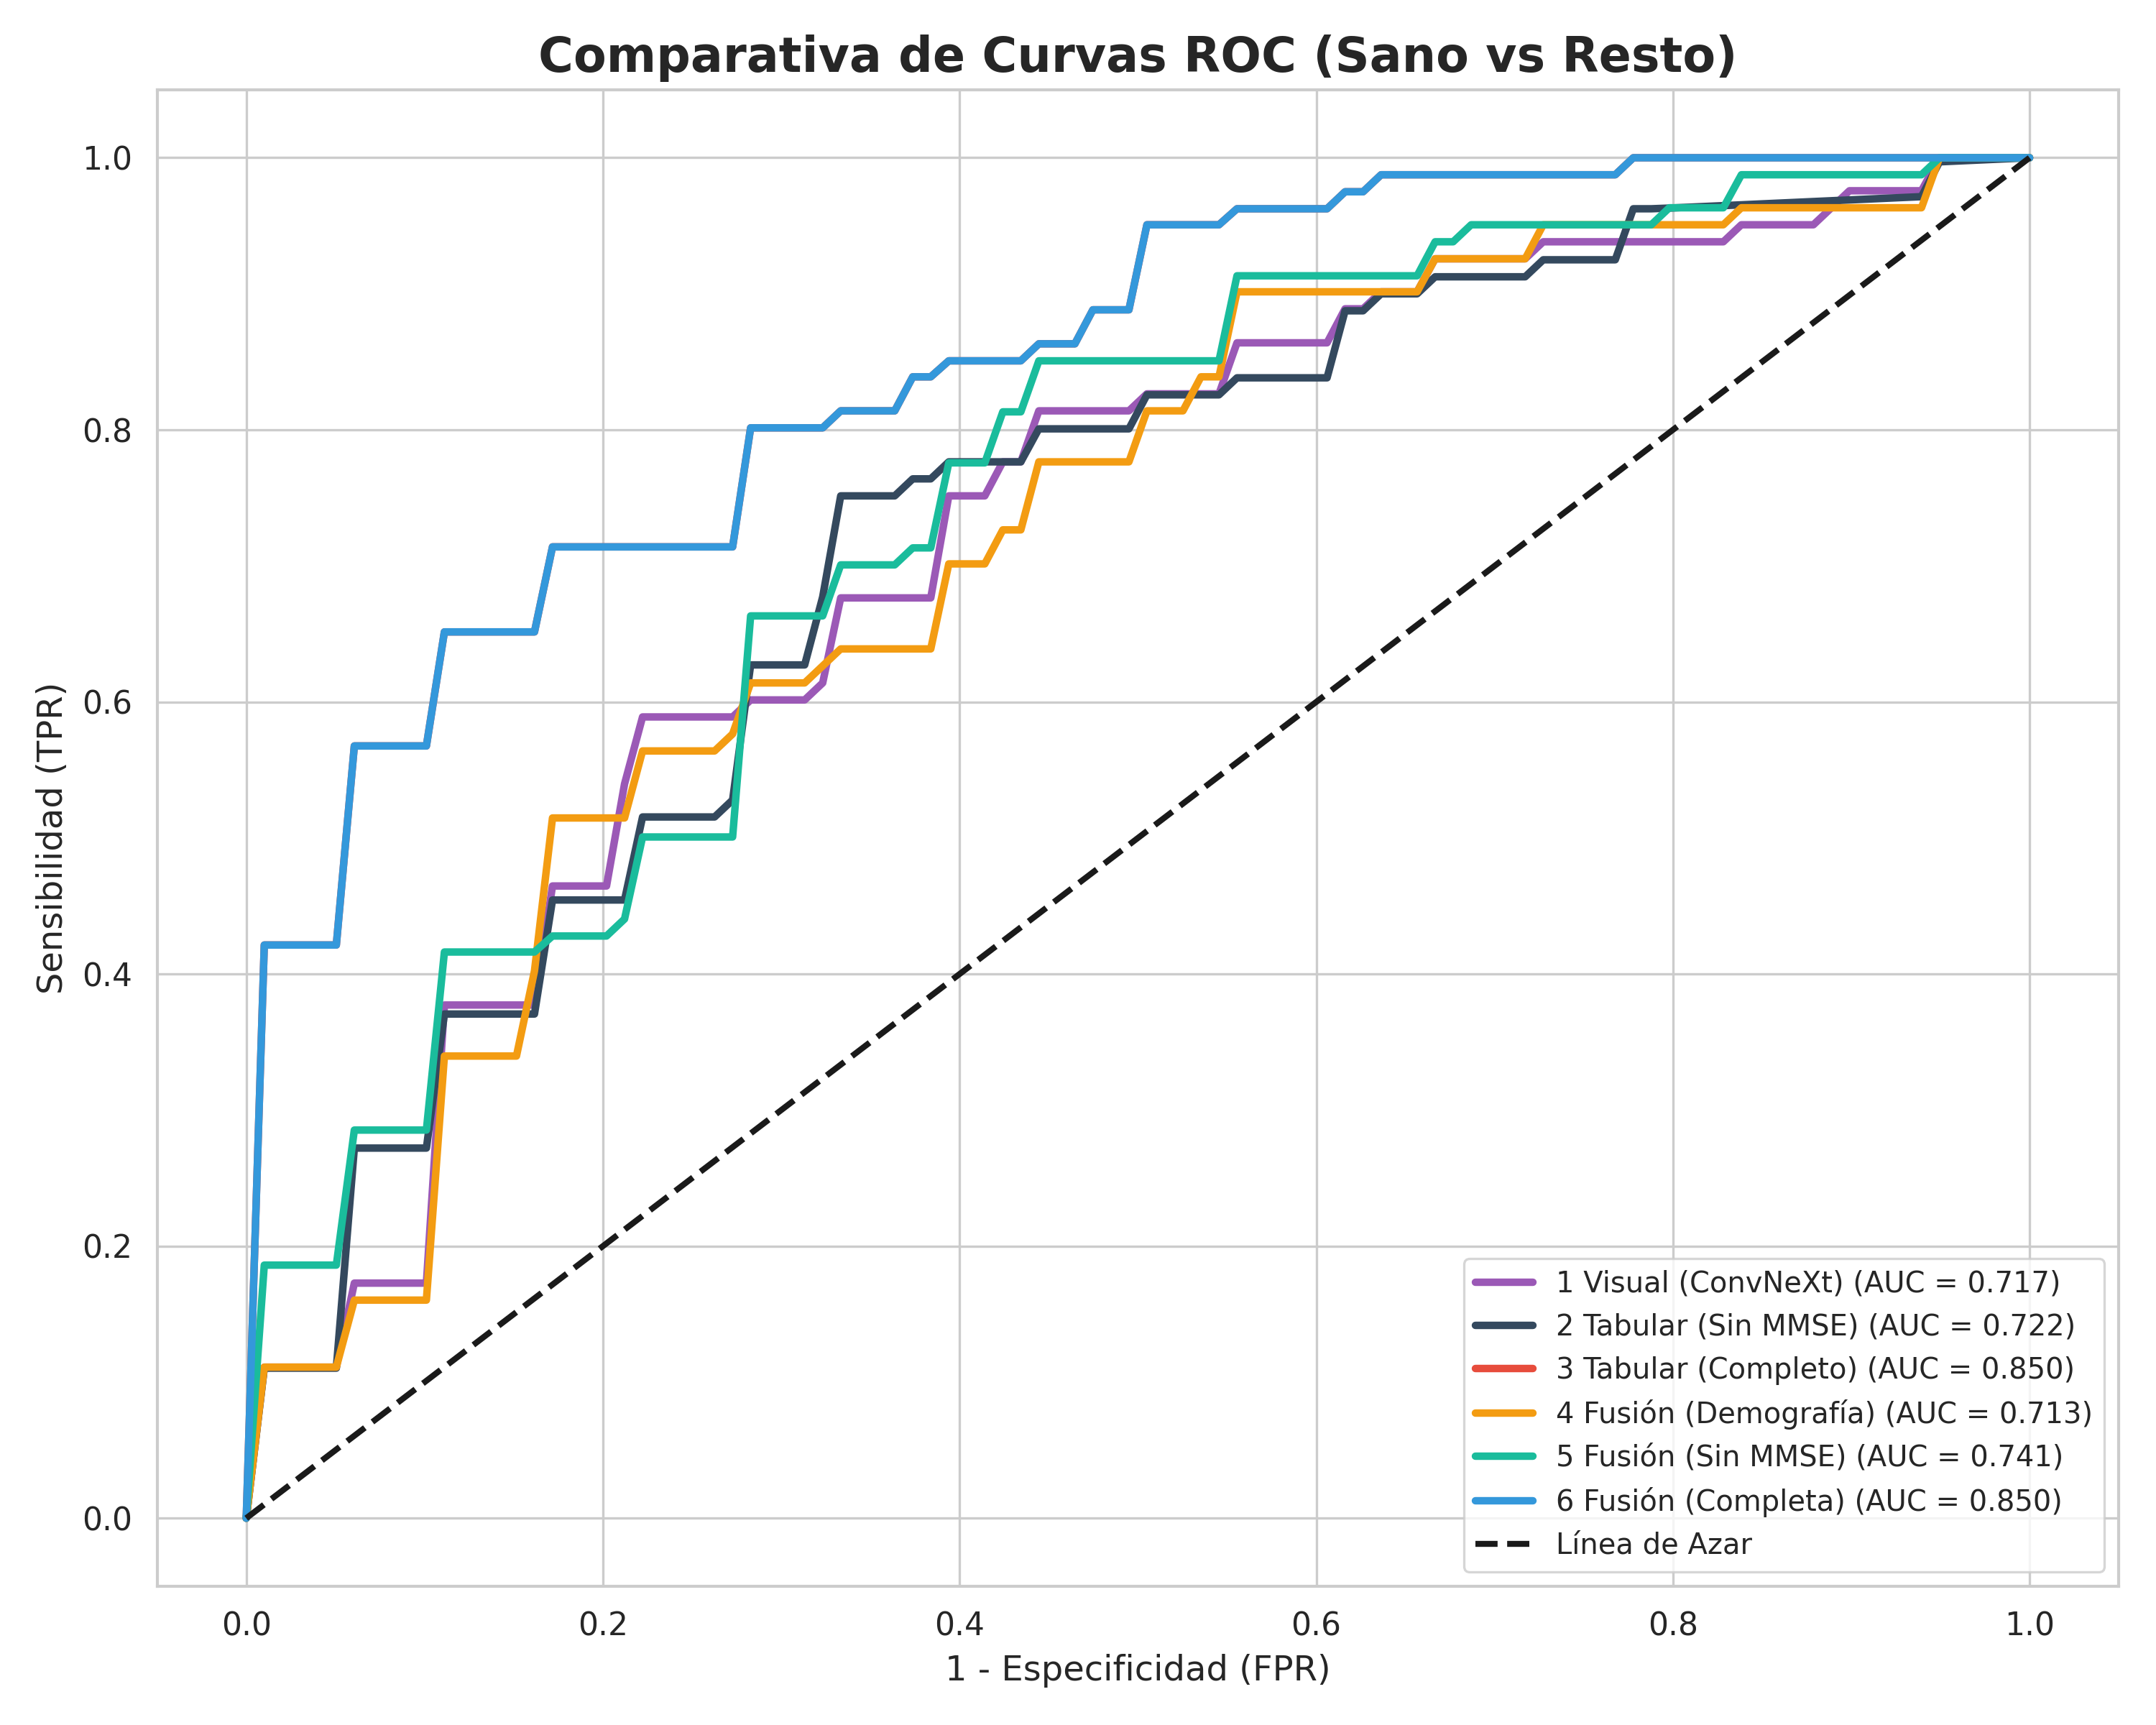
\includegraphics[width=0.9\textwidth]{imagenes/multiclase/02_ROC_Filtradas.png}
	\caption[Curvas ROC del régimen ordinal multiclase.]{\textbf{Curvas ROC (Análisis comparativo de separación global).} La superposición de las configuraciones completas evidencia la dominancia del test tabular. \textbf{Fuente:}  Elaboración propia.}
	\label{fig:roc_ordinal}
\end{figure}

Debido a las limitaciones espaciales del AUC-ROC en este dominio, la evaluación real de la consistencia del sistema se fundamenta en métricas que sí comprenden la naturaleza jerárquica del Alzheimer. La Figura \ref{fig:boxplots_mae_qwk} recoge la distribución del \textbf{Error Absoluto Medio (MAE)} y del \textbf{Coeficiente Kappa de Cohen Ponderado Cuadráticamente (QWK)} a través de todas las particiones del particionado cruzado.

\begin{figure}[htpb]
	\centering
	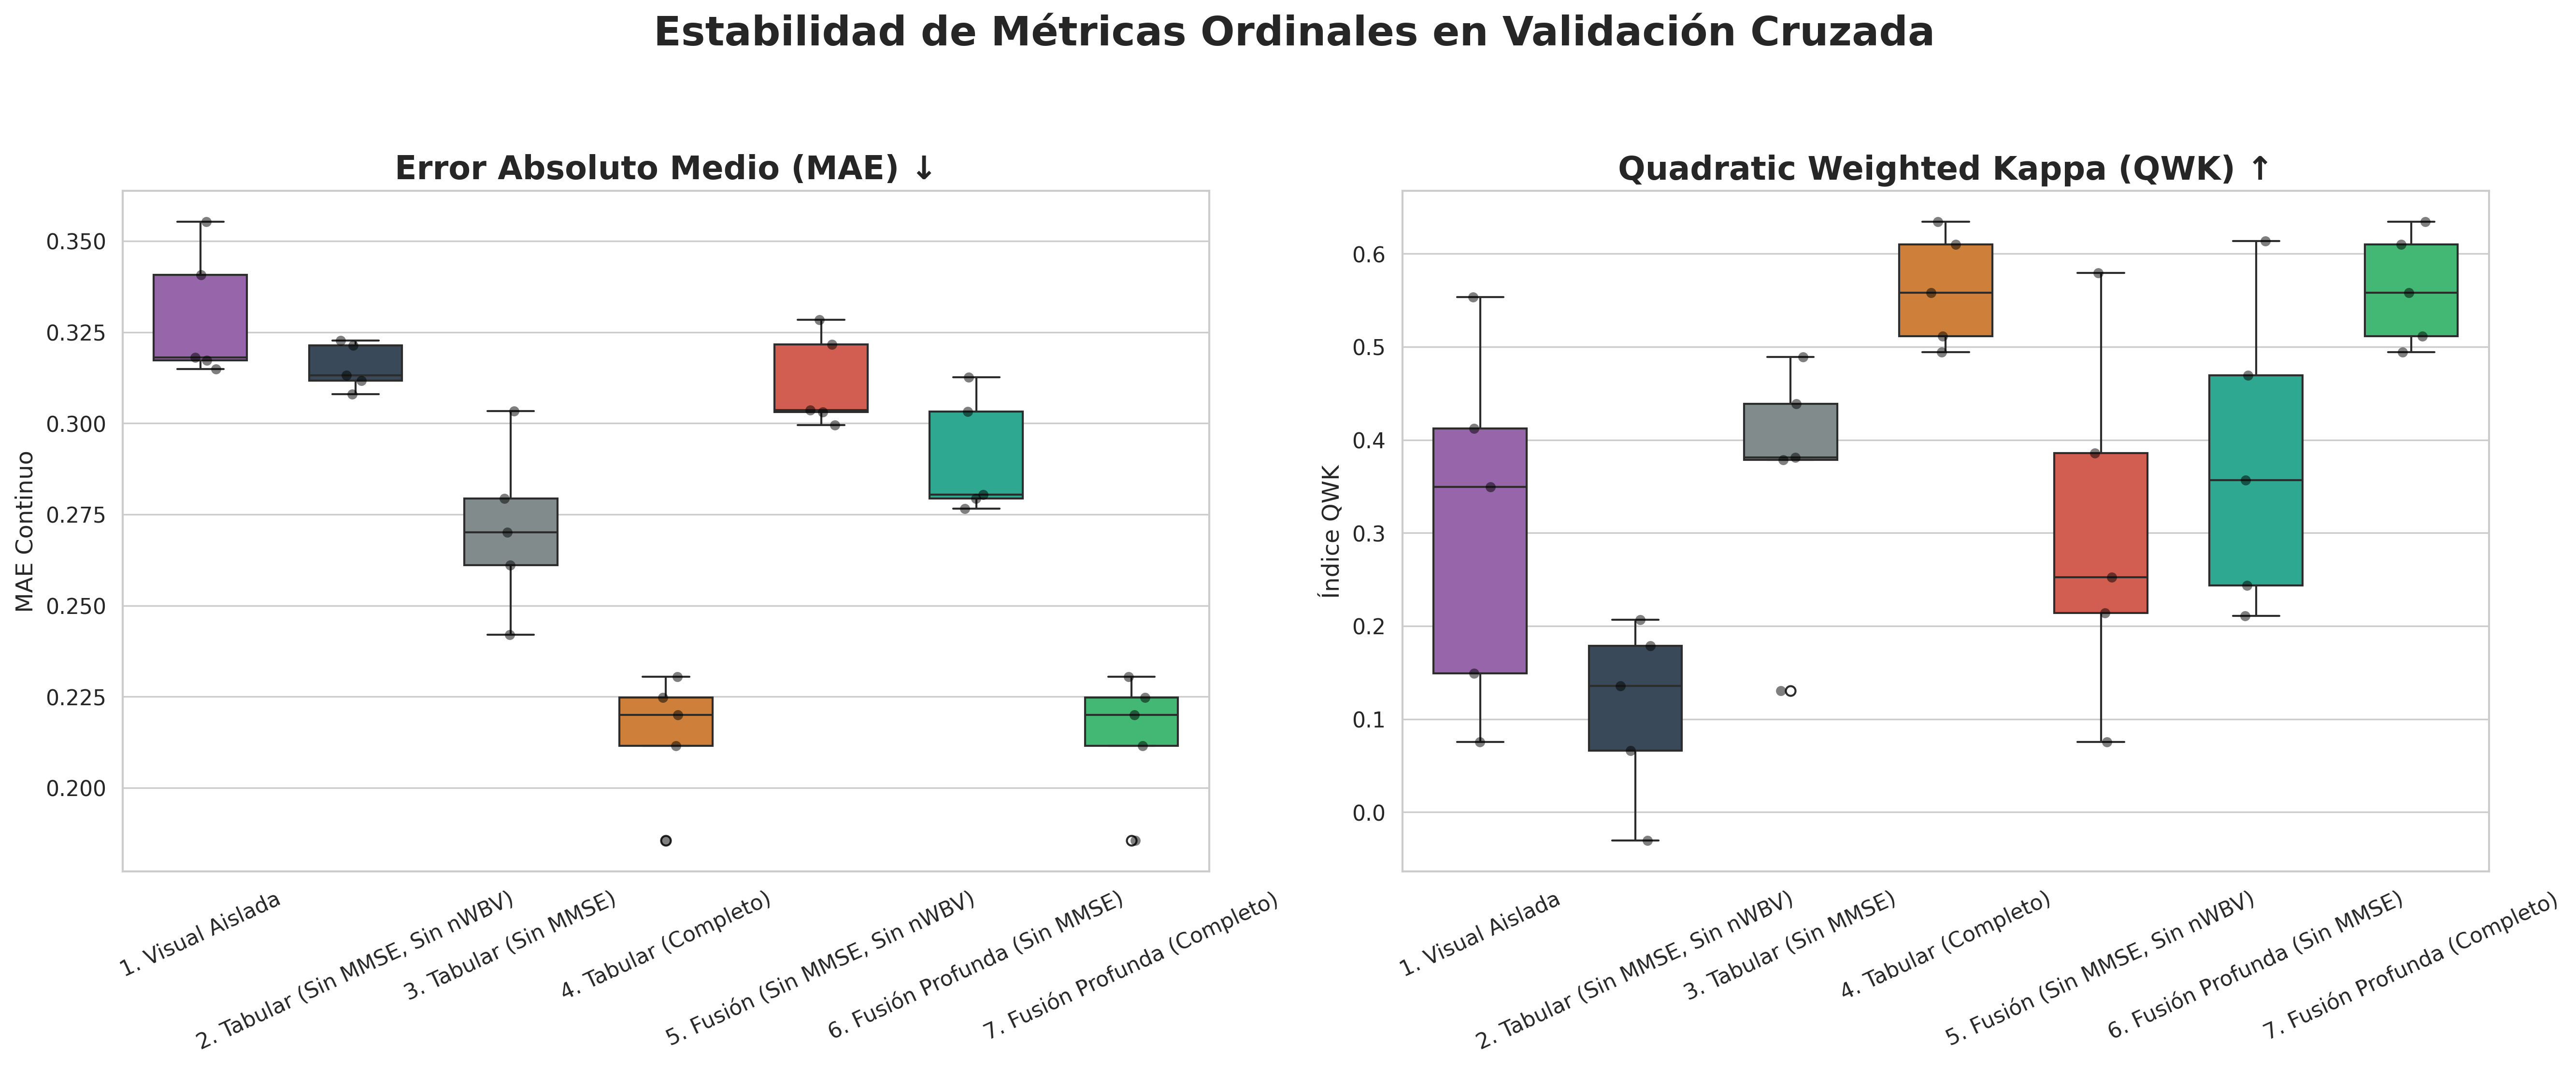
\includegraphics[width=\textwidth]{imagenes/multiclase/09_Boxplots_MAE_QWK.png}
	\caption[Estabilidad de Métricas Ordinales (MAE y QWK).] {Consistencia operativa en el continuo neurodegenerativo. El análisis de dispersión por pliegues constata el impacto de rescate de la rama visual en escenarios de privación clínica (Modelos 2 vs. 5) y la convergencia matemática idéntica del modelo híbrido hacia el canal tabular puro (Modelos 3 y 6). \textbf{Fuente:} Elaboración propia.}
	\label{fig:boxplots_mae_qwk}
\end{figure}

El perfil de distribución de las cajas refleja la consistencia de la orquestación multimodal según el escenario analizado. Se observa visualmente cómo la inclusión de la imagen en entornos sin test cognitivos (como se aprecia en el Modelo 5) estabiliza la inferencia, reduciendo el error continuo (MAE) y elevando la concordancia discreta (QWK) respecto a las aproximaciones lineales básicas. Por otro lado, la similitud en la dispersión, medianas y valores atípicos entre el Modelo Tabular Completo (Modelo 3) y la Fusión Completa (Modelo 6) constata el fenómeno de la dominancia de modalidad. En este escenario completo, el proceso de optimización prioriza la estabilidad diagnóstica derivada del test MMSE y reduce la influencia de la imagen estructural, protegiendo al sistema de variaciones innecesarias en la medición del continuo neurodegenerativo.

\begin{figure}[htpb]
	\centering
	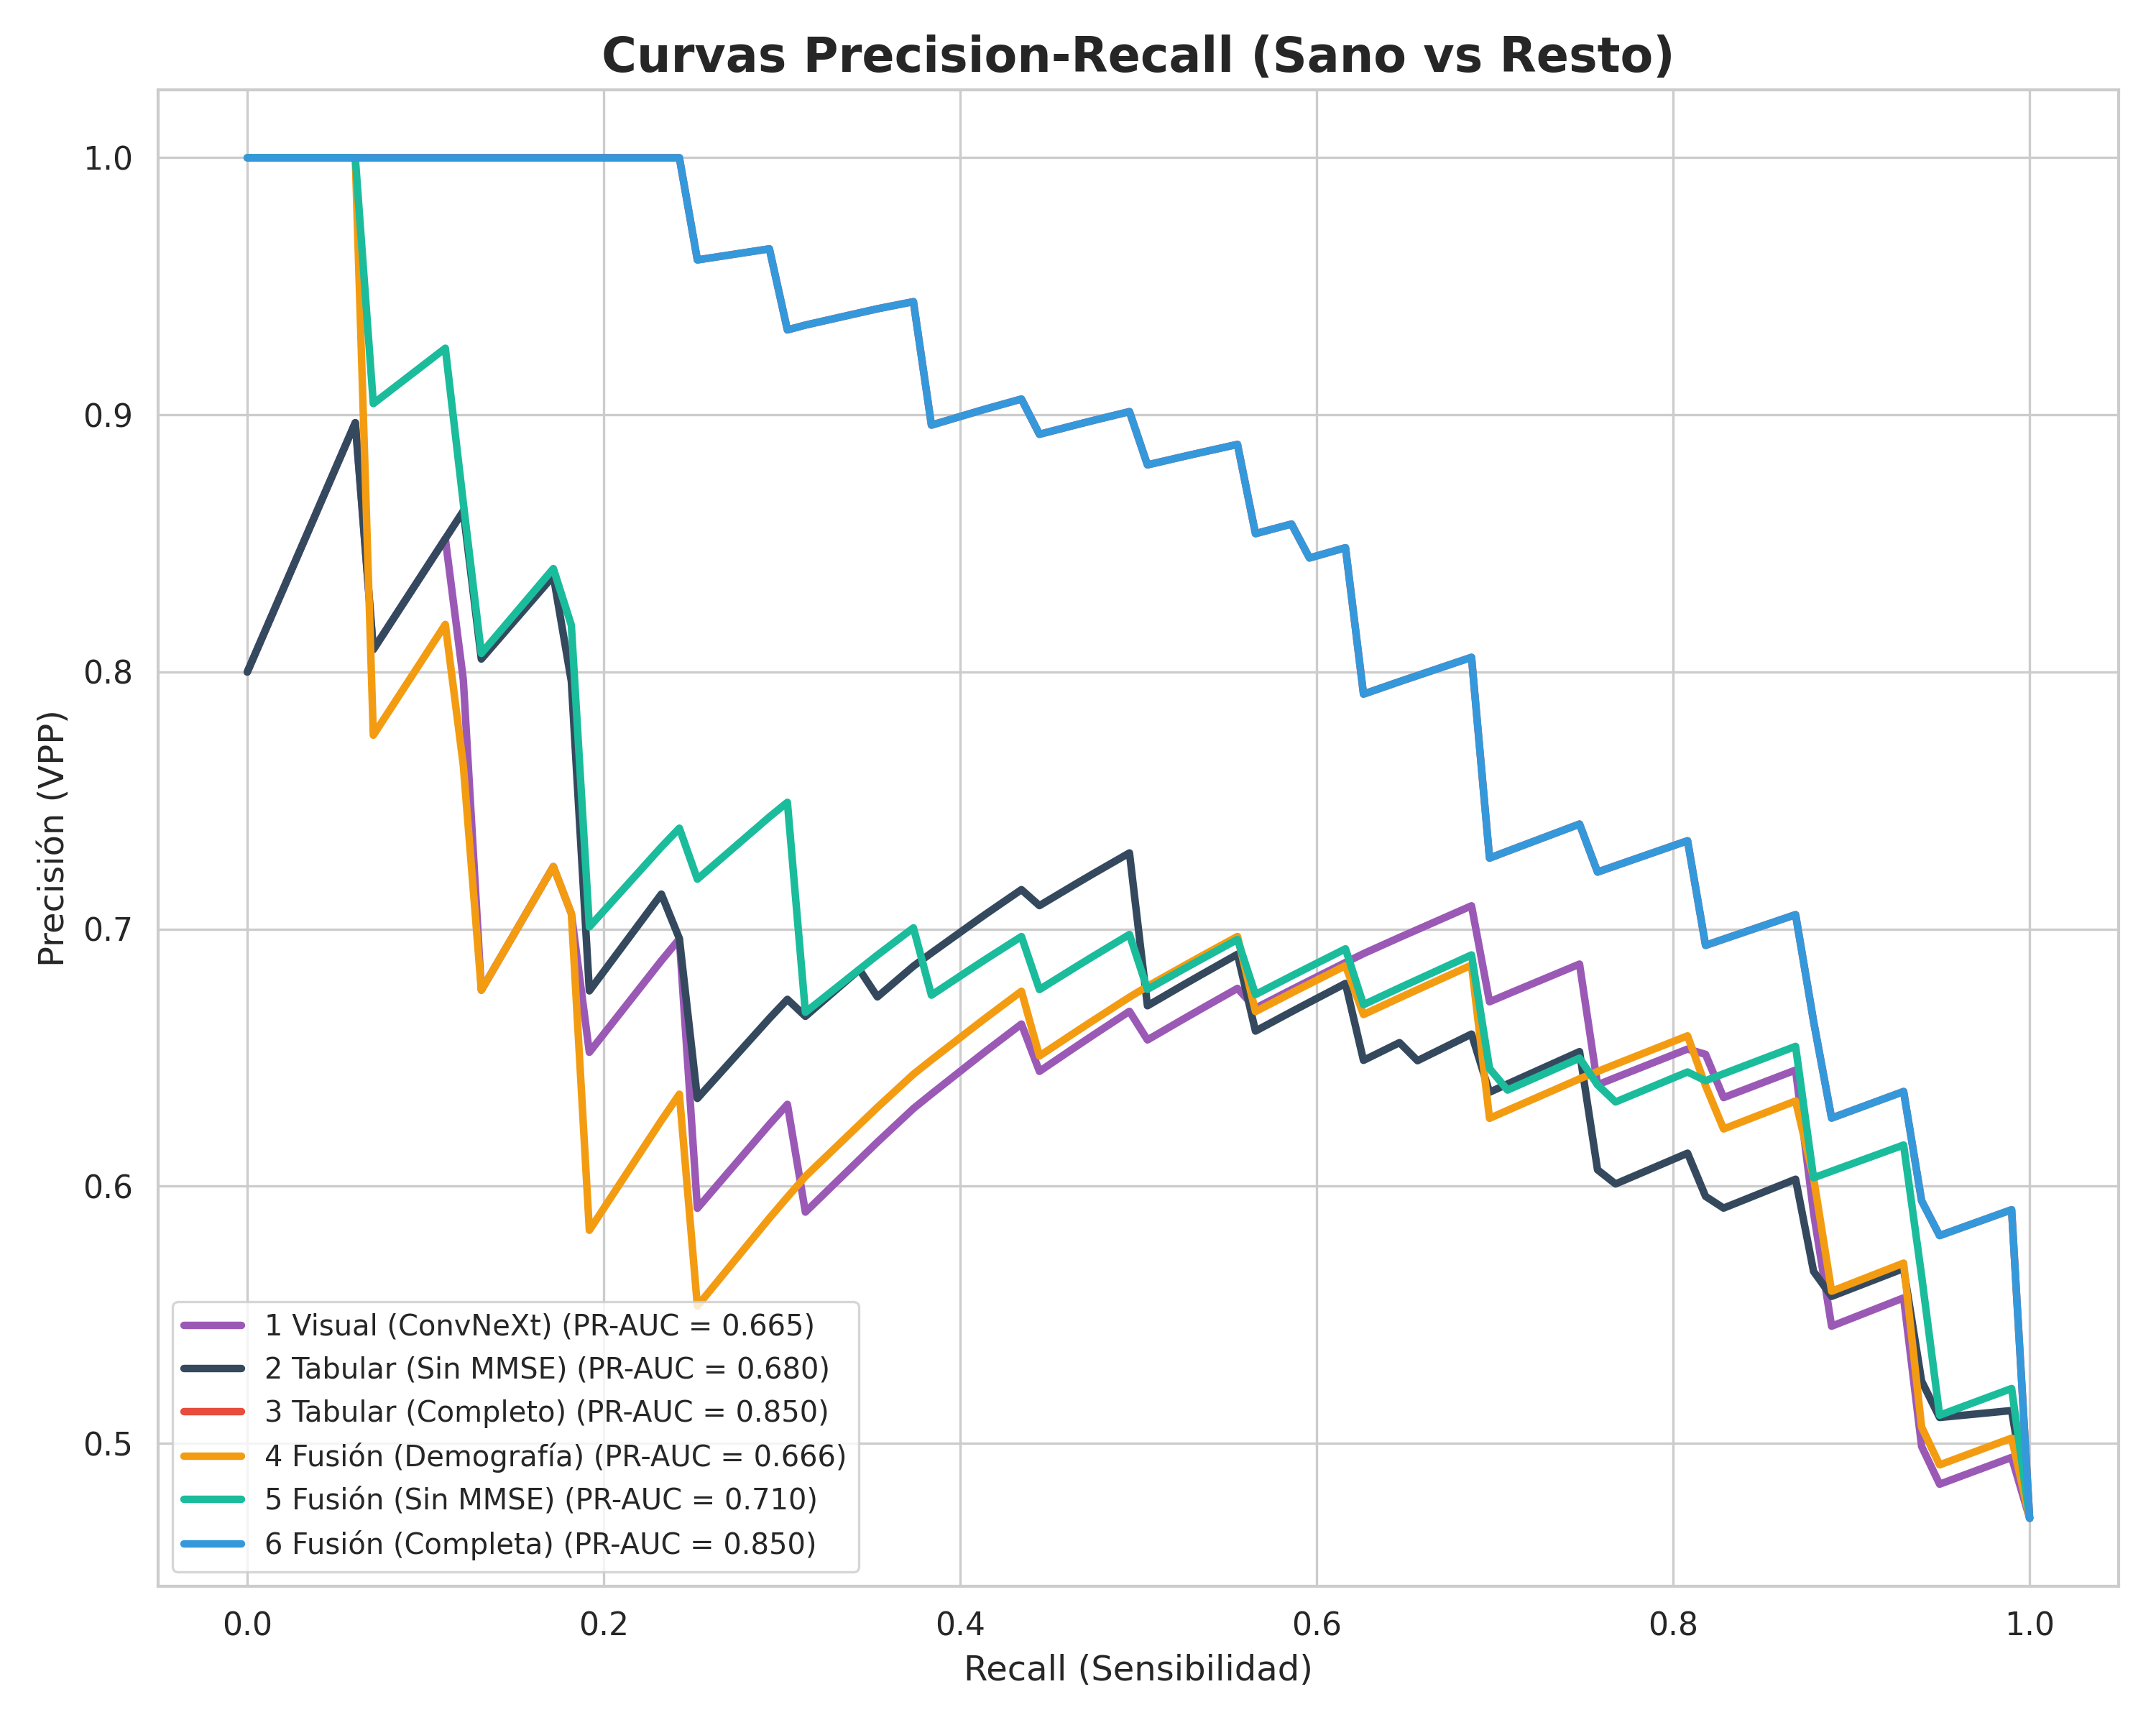
\includegraphics[width=0.9\textwidth]{imagenes/multiclase/05_PR_Filtradas.png}
	\caption[Curvas Precision-Recall del régimen ordinal multiclase.]{\textbf{Curvas Precision-Recall (Control de falsas alarmas).} La gráfica destaca la resiliencia del modelo completo ante el desbalance de clases patológicas. \textbf{Fuente:}  Elaboración propia.}
	\label{fig:pr_ordinal}
\end{figure}

Por su parte, la \textbf{curva PR} (Figura \ref{fig:pr_ordinal}) actúa como el indicador definitivo de fiabilidad ante el \textbf{desbalance de clases} inherente a la estadificación de la enfermedad. A diferencia de la ROC, este análisis evalúa la precisión (valor predictivo positivo) frente a la sensibilidad, siendo mucho más exigente al tratar con las categorías minoritarias. Al observar que los modelos completos mantienen un \textbf{PR-AUC} de \textbf{0.8505}, validamos que la arquitectura no colapsa hacia la predicción de la clase mayoritaria sana por pura conveniencia estadística. Este resultado garantiza un valor predictivo positivo robusto, esencial para asegurar que las alertas de patología emitidas por el sistema posean una alta probabilidad de ser diagnósticos reales, incluso al transitar por las complejas fronteras biológicas del Deterioro Cognitivo Leve.


\subsection{Evaluación de la Separabilidad de Densidades en la Escala Ordinal} \label{subsec:ordinal_topologia}

Para comprender la volatilidad de métricas discretas como el QWK, es imperativo revisar cómo la red organiza el espacio de decisión en un continuo matemático. La Figura \ref{fig:kde_final_ordinal} despliega la evolución de la estimación de densidad probabilística (KDE) a través de las diferentes configuraciones del sistema, mapeando la esperanza matemática ($\mathbb{E}[y]$) asignada a cada sujeto frente a su diagnóstico clínico real.


\begin{figure}[htpb]
	\centering
	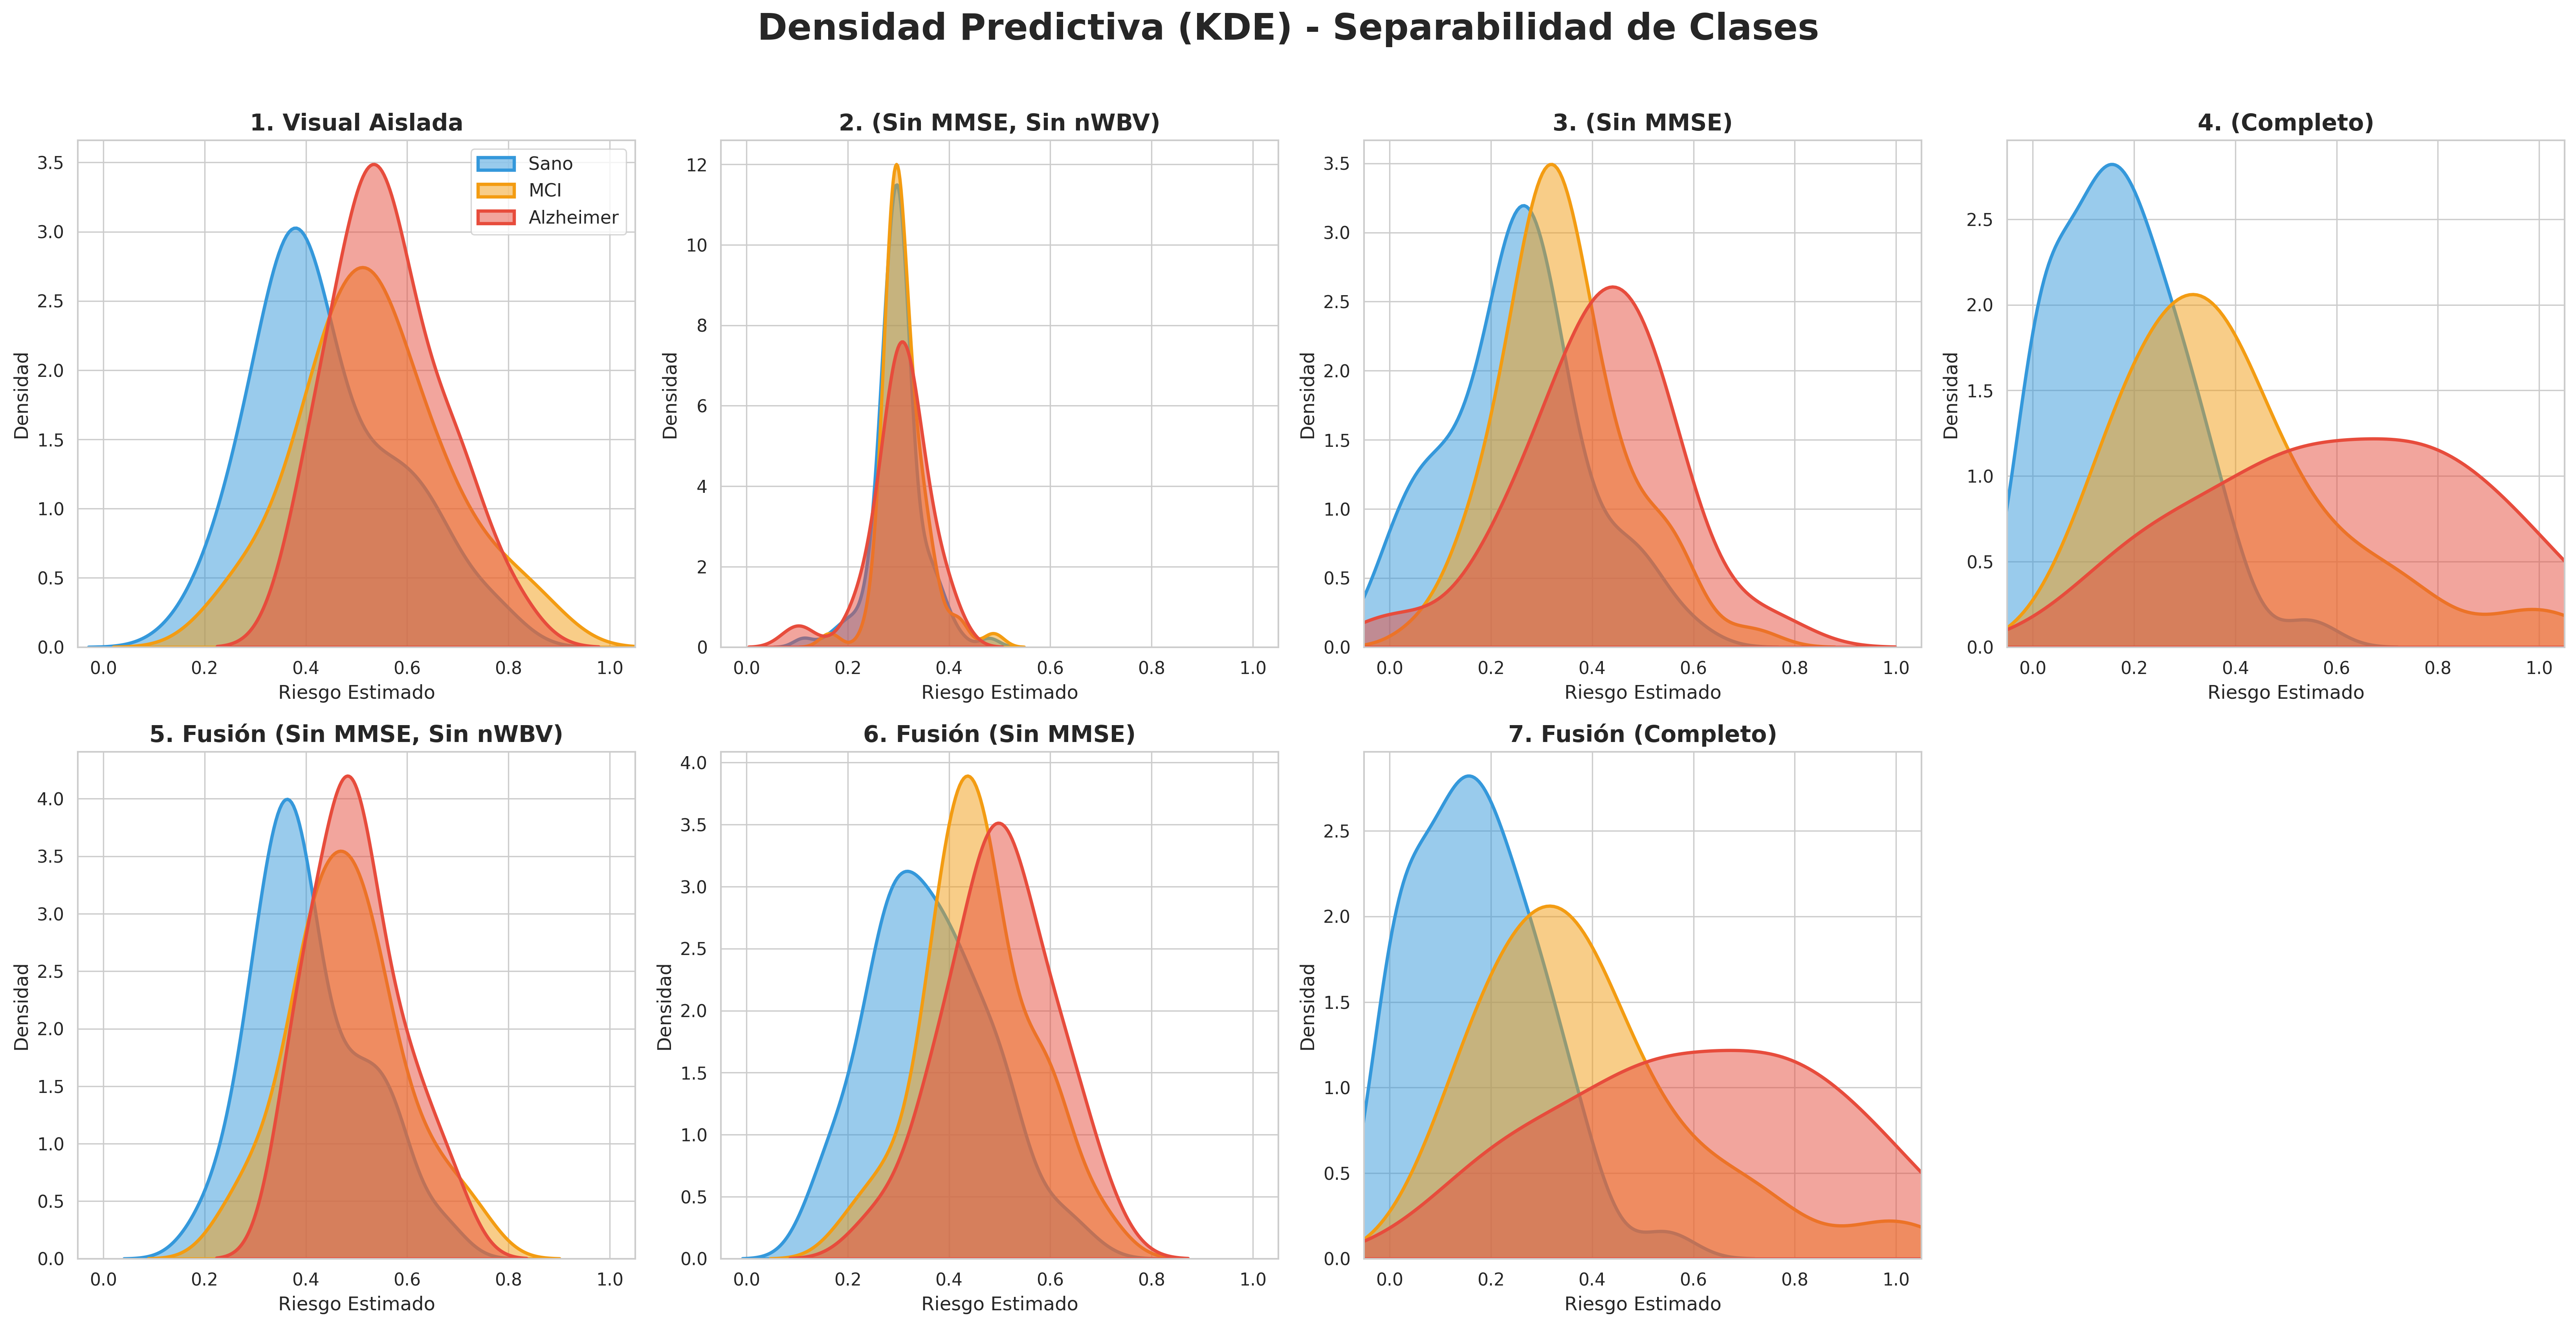
\includegraphics[width=\textwidth]{imagenes/multiclase/05_KDE_Todos_Modelos.png}
	\caption[Densidad predictiva multiclase] {Evolución de la separabilidad de clases en el régimen ordinal. El gran solapamiento del MCI ilustra la continuidad natural de la patología. \textbf{Fuente:}  Elaboración propia.}
	\label{fig:kde_final_ordinal}
\end{figure}


A lo largo de las configuraciones con mayor capacidad predictiva, se observa un fenómeno estructural constante: la clase intermedia (Deterioro Cognitivo Leve o MCI, curva naranja) no ocupa un clúster aislado, sino que actúa como un extenso puente probabilístico. Esta distribución se solapa íntimamente tanto con el envejecimiento normal sano (azul) como con la demencia establecida (rojo). La arquitectura CORAL, al analizar la severidad de la atrofia o el declive cognitivo, intenta ubicar al sujeto exactamente en ese continuo ininterrumpido.

El desglose por modelos revela dinámicas de aprendizaje sumamente interesantes que justifican el ensamblaje híbrido. El Modelo 2 (Tabular sin MMSE), que prescinde del test cognitivo pero cuenta con la variable volumétrica (nWBV), logra estructurar de forma preliminar el espectro neurodegenerativo, aunque manifiesta un solapamiento notable en las fronteras de transición debido a la sutil gradación de la atrofia transversal. Sin embargo, al observar el comportamiento de la \textbf{Fusión sin MMSE (Modelo 5)}, la inyección ponderada de la neuroimagen estructural mediante el orquestador estabiliza y refina la separación de las densidades, forzando una distribución más ordenada de las clases a lo largo del continuo. 

En el extremo superior del rendimiento, la \textbf{Fusión Completa (Modelo 6)}, que replica la topología del Modelo 3 debido a la dominancia de la modalidad clínica anteriormente mencionada, exhibe la distribución más definida: la masa probabilística de los sujetos sanos se ancla firmemente hacia el origen, los pacientes con demencia se desplazan hacia el segmento superior, y el MCI vertebra la transición de forma escalonada, minimizando los saltos catastróficos de clasificación.

\subsection{Estabilidad del Aprendizaje, Calibración y Error} \label{subsec:estabilidad_ordinal}

\begin{figure}[htpb]
	\centering
	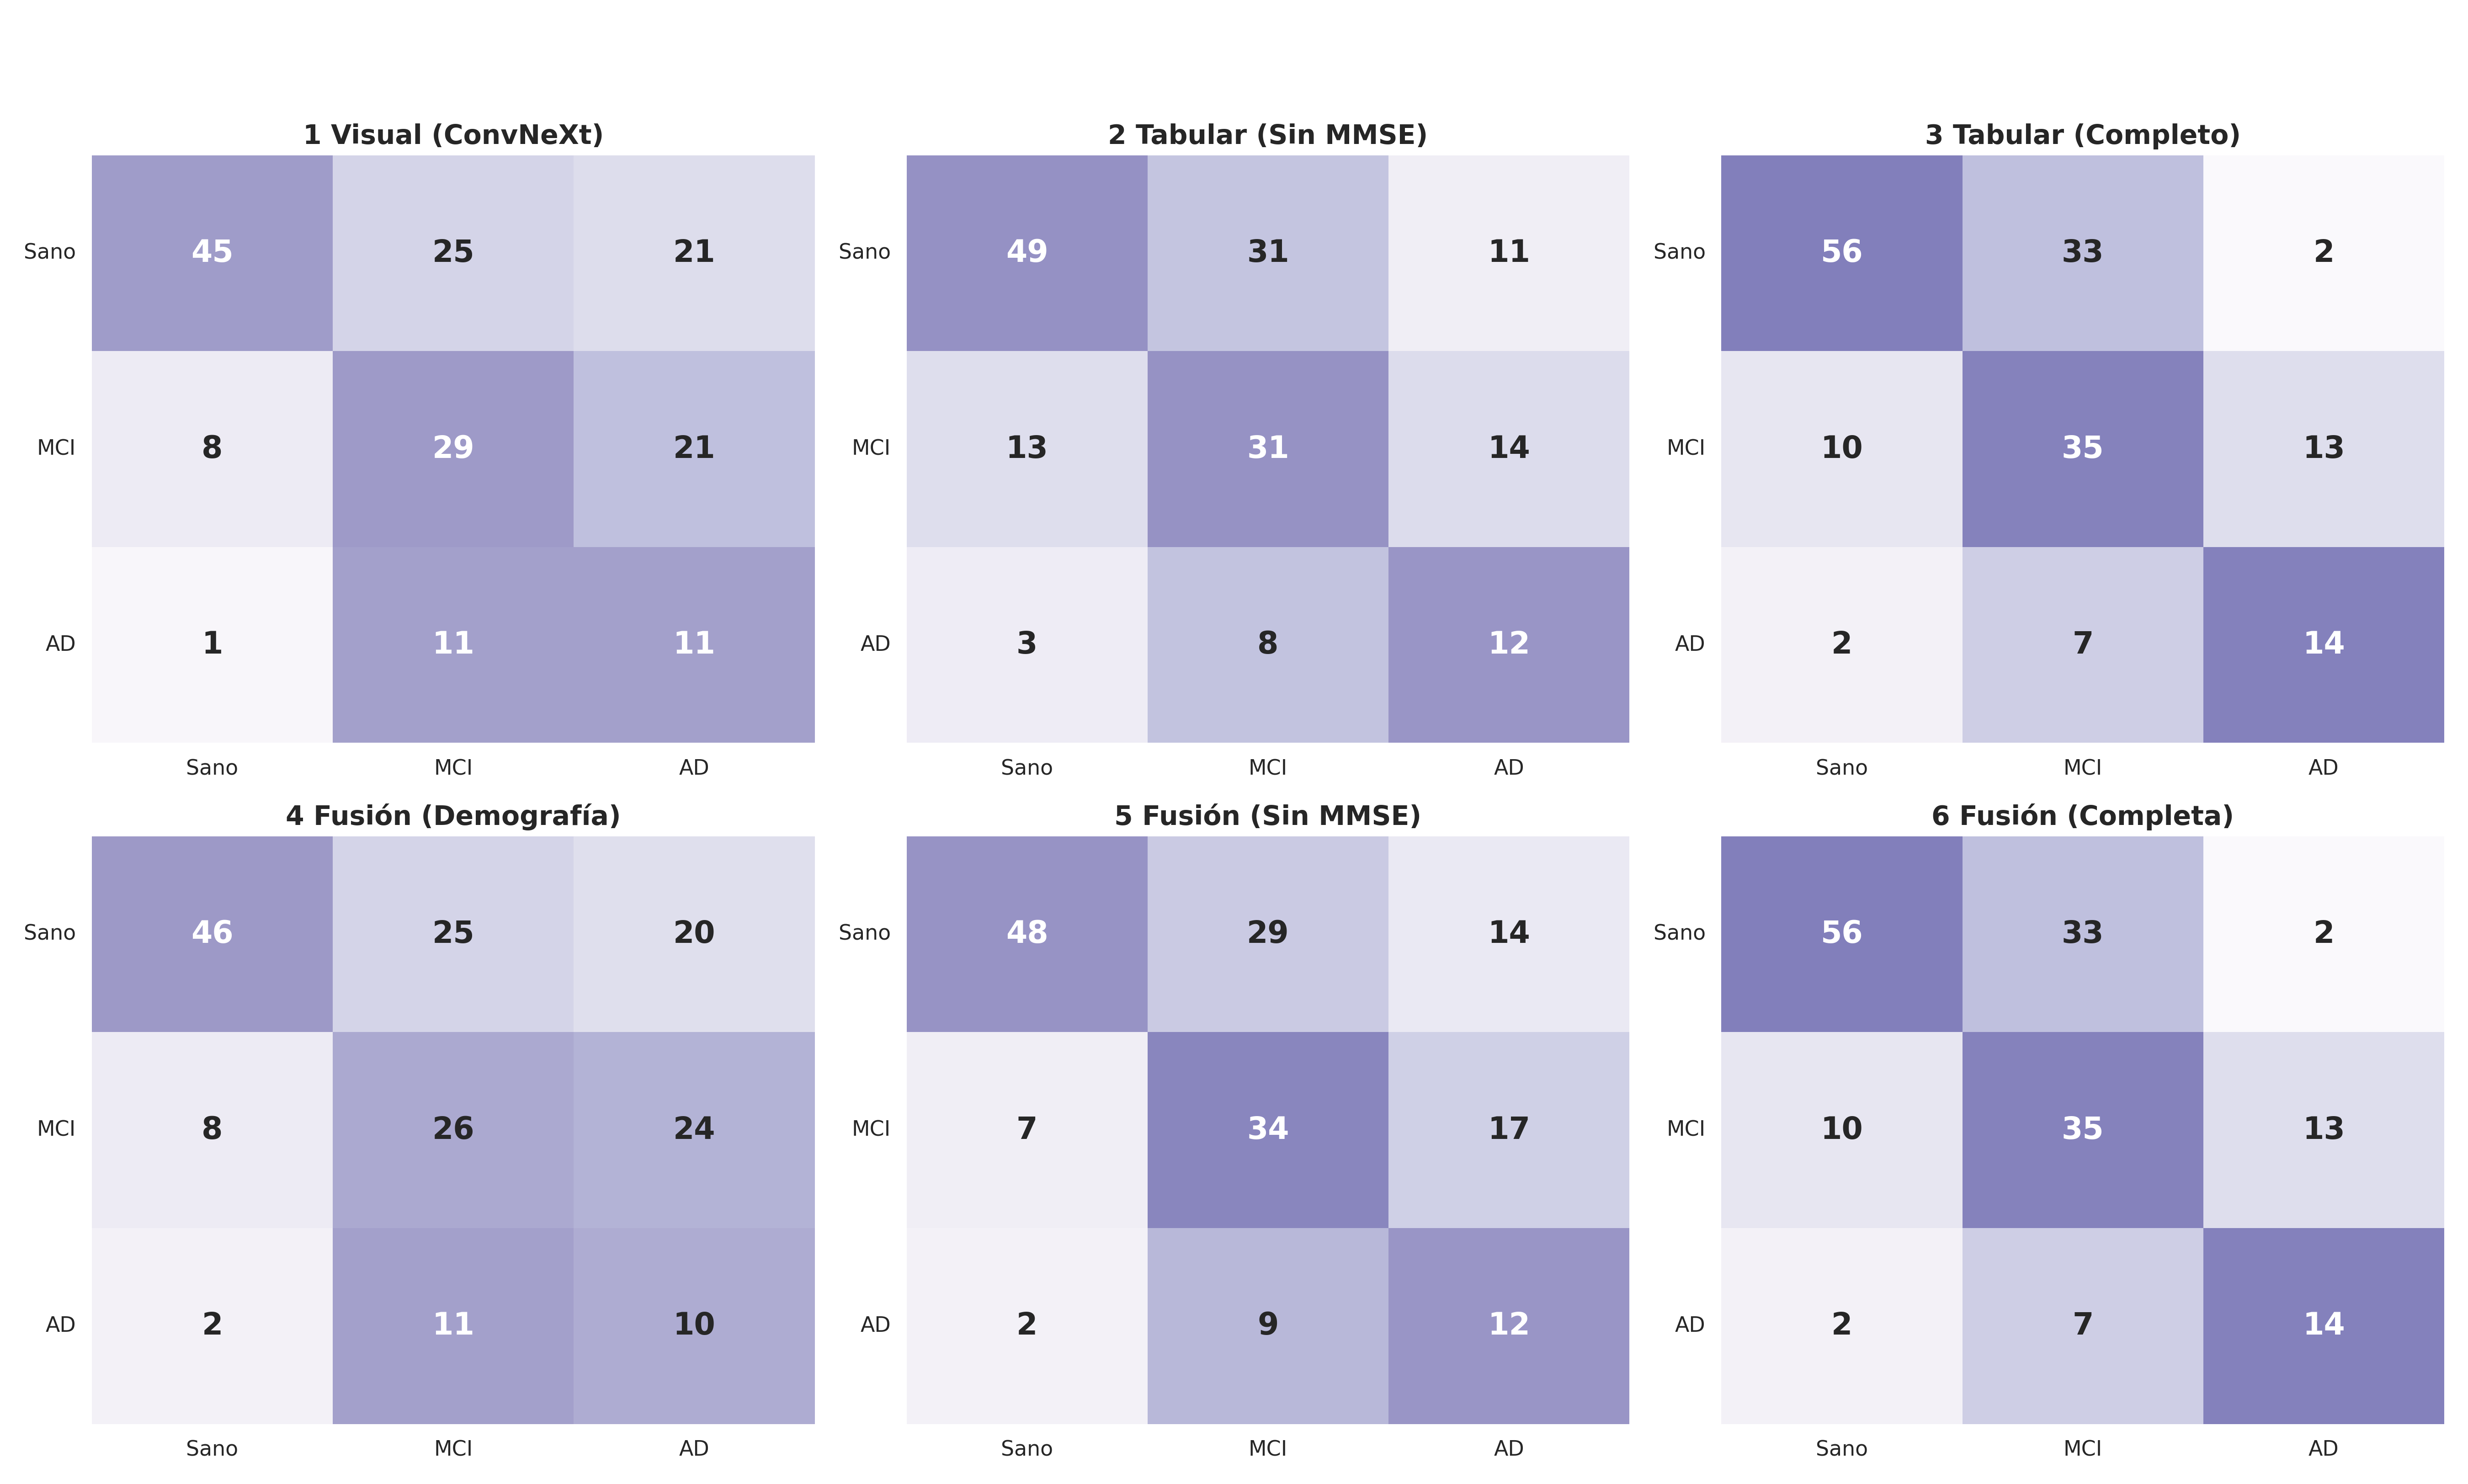
\includegraphics[width=\textwidth]{imagenes/multiclase/03_Matrices_Limpias.png}
	\caption[Matrices de Confusión en Régimen Ordinal.] {Revisión del error multiclase OOF discretizado. Se observa la progresiva diagonalización. \textbf{Fuente:} Elaboración propia.}
	\label{fig:matrices_confusion_ordinal}
\end{figure}

La inspección de las matrices de confusión multiclase (Figura \ref{fig:matrices_confusion_ordinal}) permite analizar el comportamiento del sistema frente a la continuidad de la enfermedad. Es fundamental recordar que, mientras el hiperparámetro de fusión ($W_{vis}$) se ajusta para minimizar el error absoluto continuo, la asignación final del paciente a un estadio clínico discreto se rige por una estrategia de optimización dinámica. Esta estrategia adapta los umbrales de decisión para intentar equilibrar la sensibilidad sobre la clase con menos pacientes (Demencia Avanzada, AD). En este contexto, el análisis de la regresión ordinal no radica únicamente en contar los aciertos de la diagonal principal, sino en evaluar la contención estructural del error: comprobar si las clasificaciones incorrectas se limiten a estadios adyacentes (errores de un solo nivel de diferencia) o si ocurren fallos graves (como confundir a un paciente sano con uno en fase de demencia severa).

Al observar la matriz del \textbf{Modelo 2} (Tabular sin MMSE), la ausencia de métricas neuropsicológicas genera una dispersión visible en las fronteras de decisión. Al introducir la neuroimagen en la \textbf{Fusión sin MMSE (Modelo 5)}, el comportamiento cambia de forma selectiva: no se reduce el error extremo de clasificar sanos como AD (que sube sutilmente de 11 a 14), pero se logra una mejora en la identificación del estadio intermedio (MCI). El Modelo 5 incrementa los aciertos en MCI de 31 a 34 y reduce drásticamente sus falsos negativos (pacientes con MCI clasificados como sanos, que bajan de 13 a 7). Esto refleja que la combinación multimodal ayuda a estabilizar la detección de las fases de transición cuando no se dispone del test cognitivo principal.

Por otro lado, la comparativa entre el \textbf{Modelo 3} (Tabular Completo) y el \textbf{Modelo 6} (Fusión Completa) escenifica de forma exacta el fenómeno de \textbf{Dominancia de Modalidad} (\textit{Modality Laziness}). Al anular el peso visual ($W_{vis} = 0.000$), la matriz de la Fusión Completa replica de manera idéntica cada celda de la estructura tabular. Aunque el sistema prescinde de la imagen como regulador morfológico, esta convergencia matemática asegura la consistencia diagnóstica apoyándose en la alta fiabilidad estadística que el test MMSE aporta al modelo para la separación de los tres estadios.

Para garantizar que las predicciones del sistema sean clínicamente viables, es necesario evaluar tanto la estabilidad de su entrenamiento como la honestidad de sus probabilidades (Figura \ref{fig:loss_ordinal}). 

\begin{figure}[htpb]
	\centering
	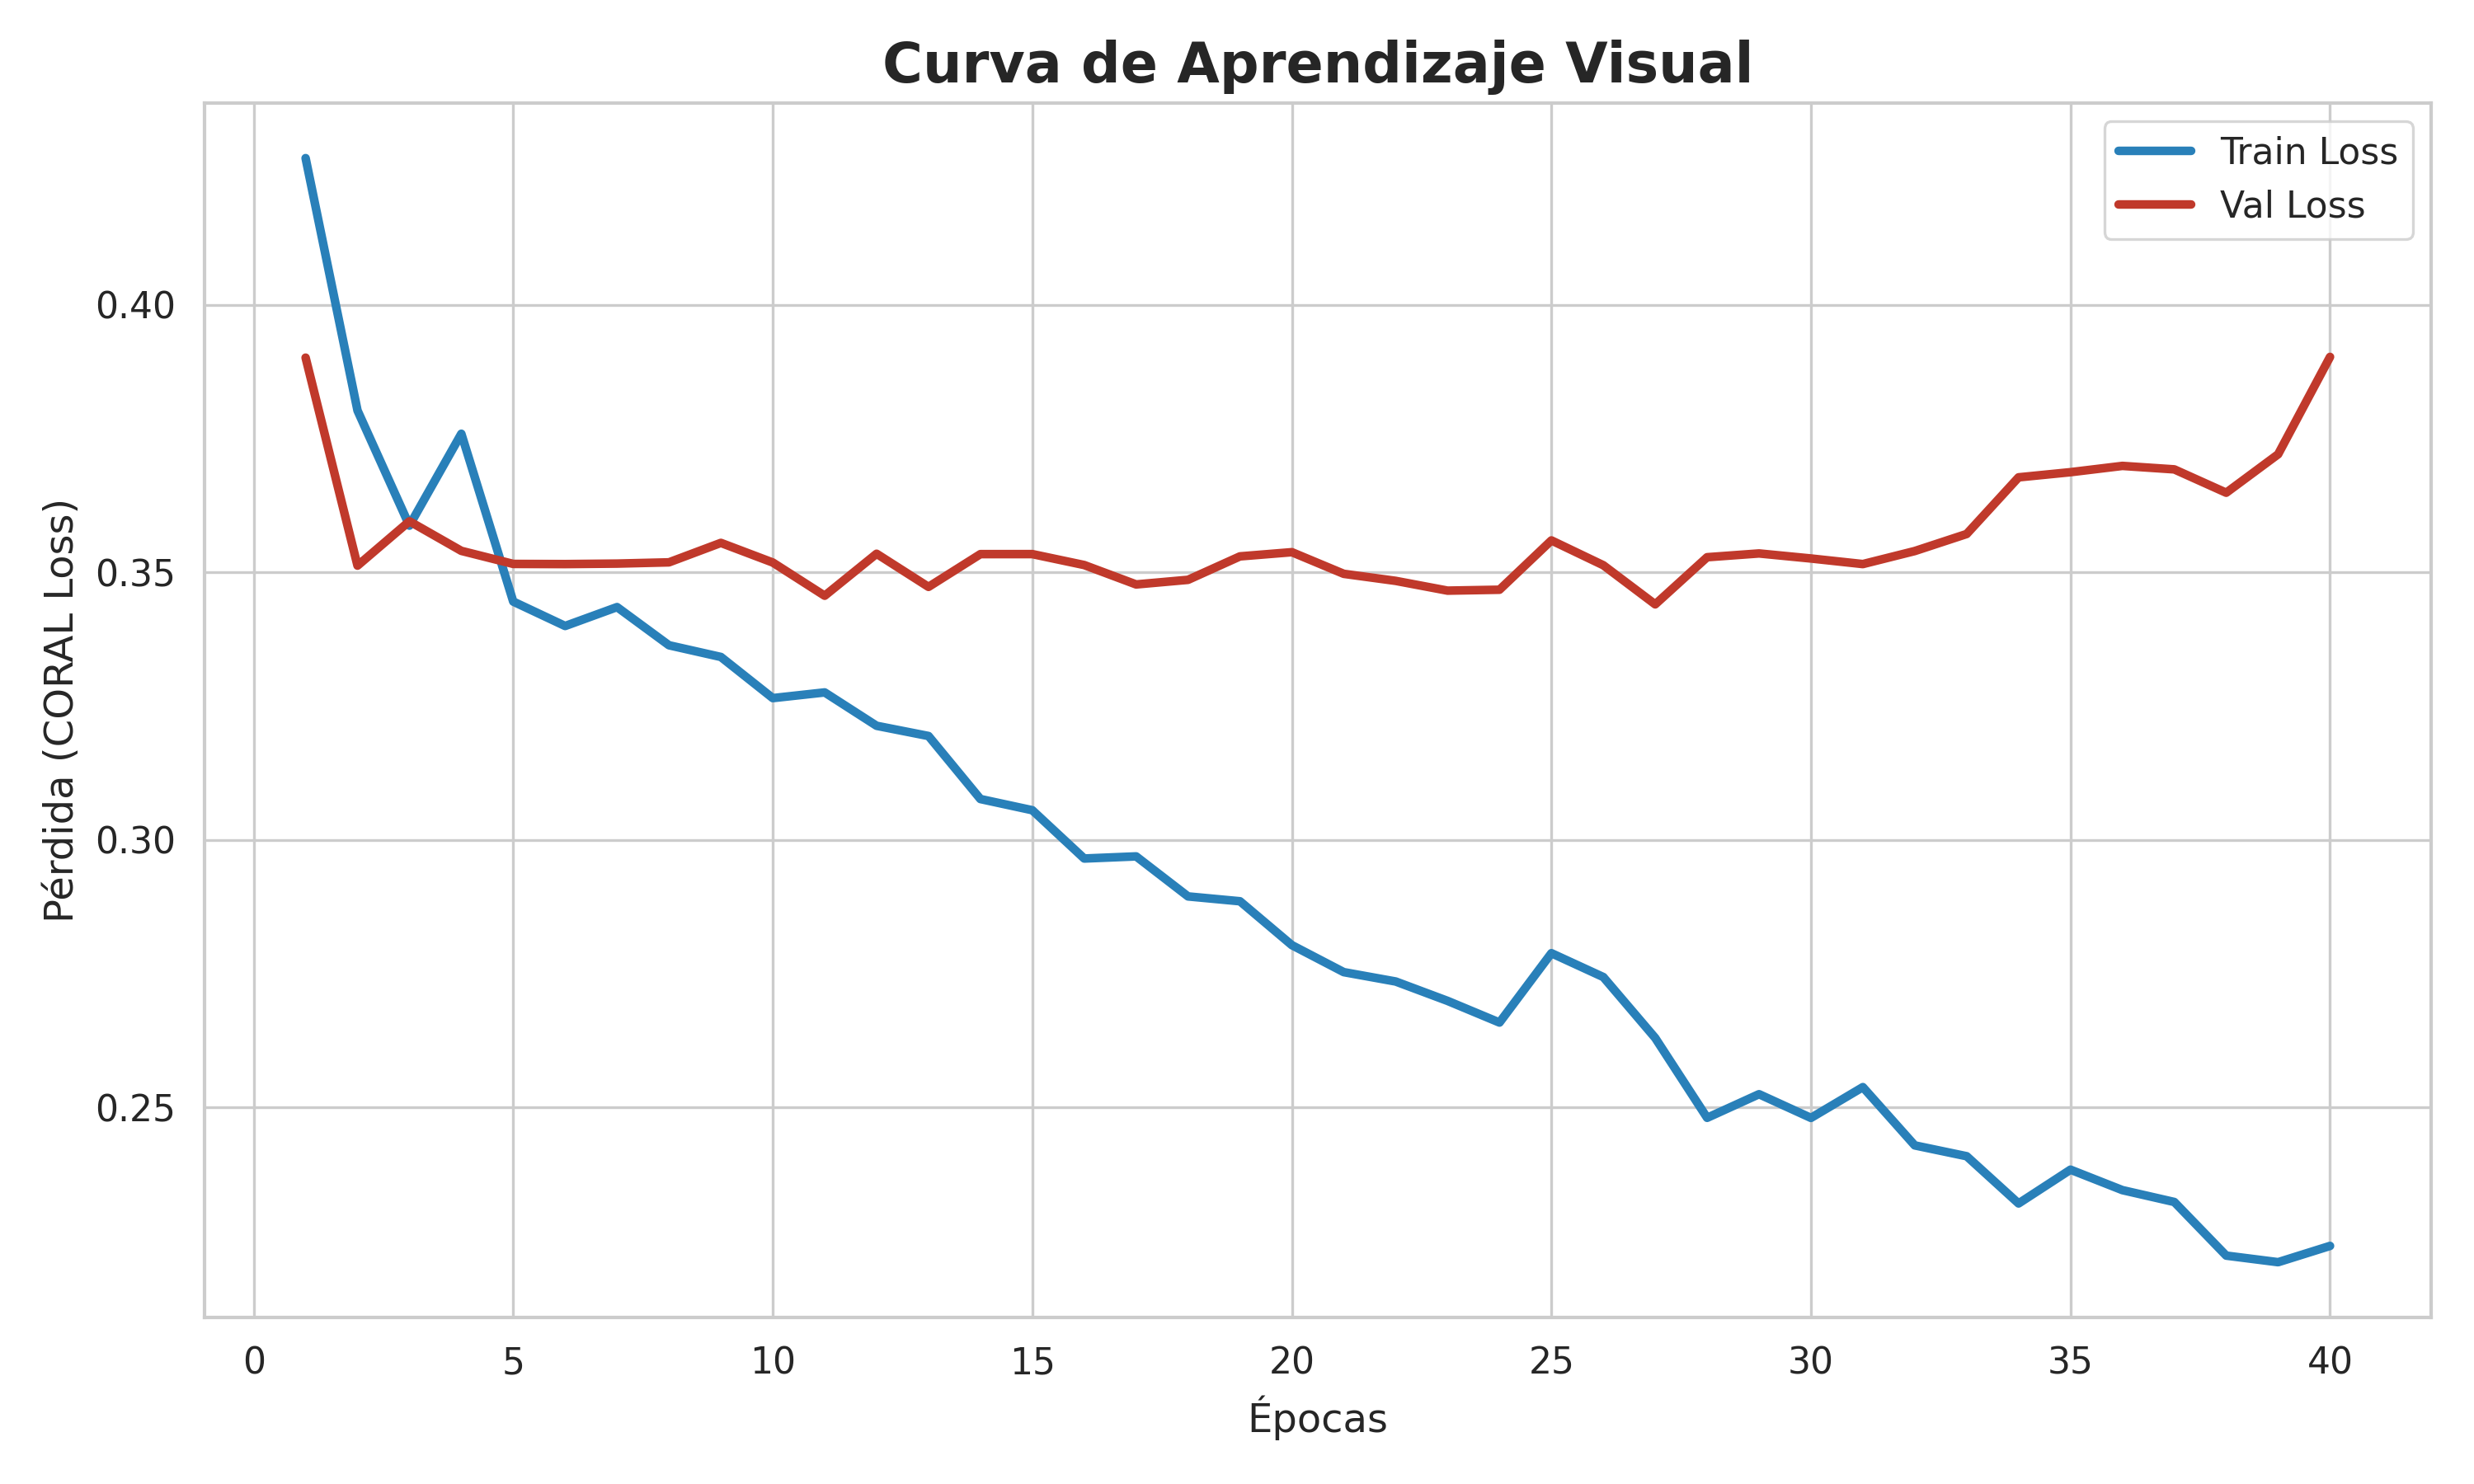
\includegraphics[width=0.75\textwidth]{imagenes/multiclase/01_Curva_Loss (1).png}
	\caption[Dinámica de pérdida CORAL en régimen ordinal.] {Evolución de la pérdida CORAL durante el entrenamiento y la validación. La estabilización temprana y el repunte final de la validación a partir de la época 32 evidencian el inicio de sobreajuste, justificando el uso de parada temprana (\textit{early stopping}) para asegurar la generalización. \textbf{Fuente:} Elaboración propia.}
	\label{fig:loss_ordinal}
\end{figure}


La dinámica de optimización visual (Figura \ref{fig:loss_ordinal}) refleja de forma nítida la complejidad intrínseca de la regresión ordinal multiclase. A diferencia de la estabilidad del escenario binario, la pérdida CORAL en validación encuentra su mínimo absoluto de manera prematura en la época 2, estableciéndose a partir de ahí en una meseta constante en torno a 0.35. Sin embargo, a partir de la época 32 se observa una divergencia clara que marca el inicio de un sobreajuste (\textit{overfitting}) tardío, donde la pérdida de validación asciende mientras la de entrenamiento continúa su descenso. Este comportamiento es un síntoma clásico de los regímenes de datos limitados: la red extrae con rapidez la varianza anatómica disponible y empieza a memorizar la muestra, confirmando la necesidad de implementar estrategias de parada temprana para congelar los pesos en su punto exacto de máxima generalización.


\subsection{Valor de Rescate y Dominancia de Modalidad} \label{subsec:ordinal_dinamica_multimodal}

El hiperparámetro de mezcla $W_{vis}$, ajustado en este régimen mediante la minimización del Error Absoluto Medio (MAE), arroja luz sobre el comportamiento interno del sistema ante la incertidumbre clínica. La evolución de este peso a lo largo de los escenarios evidencia un modelo altamente adaptativo que modula su confianza en la neuroimagen en estricta función de la debilidad del vector tabular.

En entornos de privación clínica, la imagen asume un papel crítico. En el Modelo 5 (Fusión sin MMSE), el sistema halla un punto de equilibrio multimodal ($W_{vis} = 0.594$) al integrar la cuantificación volumétrica global (nWBV) con el mapa de atrofia espacial extraído por el modelo visual. Esta combinación permite compensar la ausencia de test cognitivos, logrando una estructura predictiva más estable que se apoya en la complementariedad entre los datos tabulares disponibles y la información estructural de la neuroimagen.

No obstante, la irrupción del test cognitivo MMSE en el modelo de Fusión Completa (Modelo 6) provoca un cambio drástico. Ante la potencia predictiva de esta variable, el optimizador decide anular por completo la contribución visual, asignando un peso de $W_{vis} = 0.000$. Este comportamiento empírico ilustra el fenómeno documentado en la literatura como Dominancia de Modalidad (\textit{Modality Laziness}, detallado en la Sección \ref{subsec:sota_colapso_multimodal}). El modelo detecta que la correlación estadística del cuestionario clínico con las etiquetas ordinales es lo suficientemente sólida como para que la inclusión de la neuroimagen pueda introducir varianza o ruido paramétrico innecesario. Por lo tanto, este ajuste hacia un peso nulo actúa como un mecanismo de auto-regulación: el algoritmo prioriza la estabilidad de la métrica clínica para evitar una transferencia negativa, garantizando la consistencia del diagnóstico final.

\begin{figure}[htpb]
	\centering
	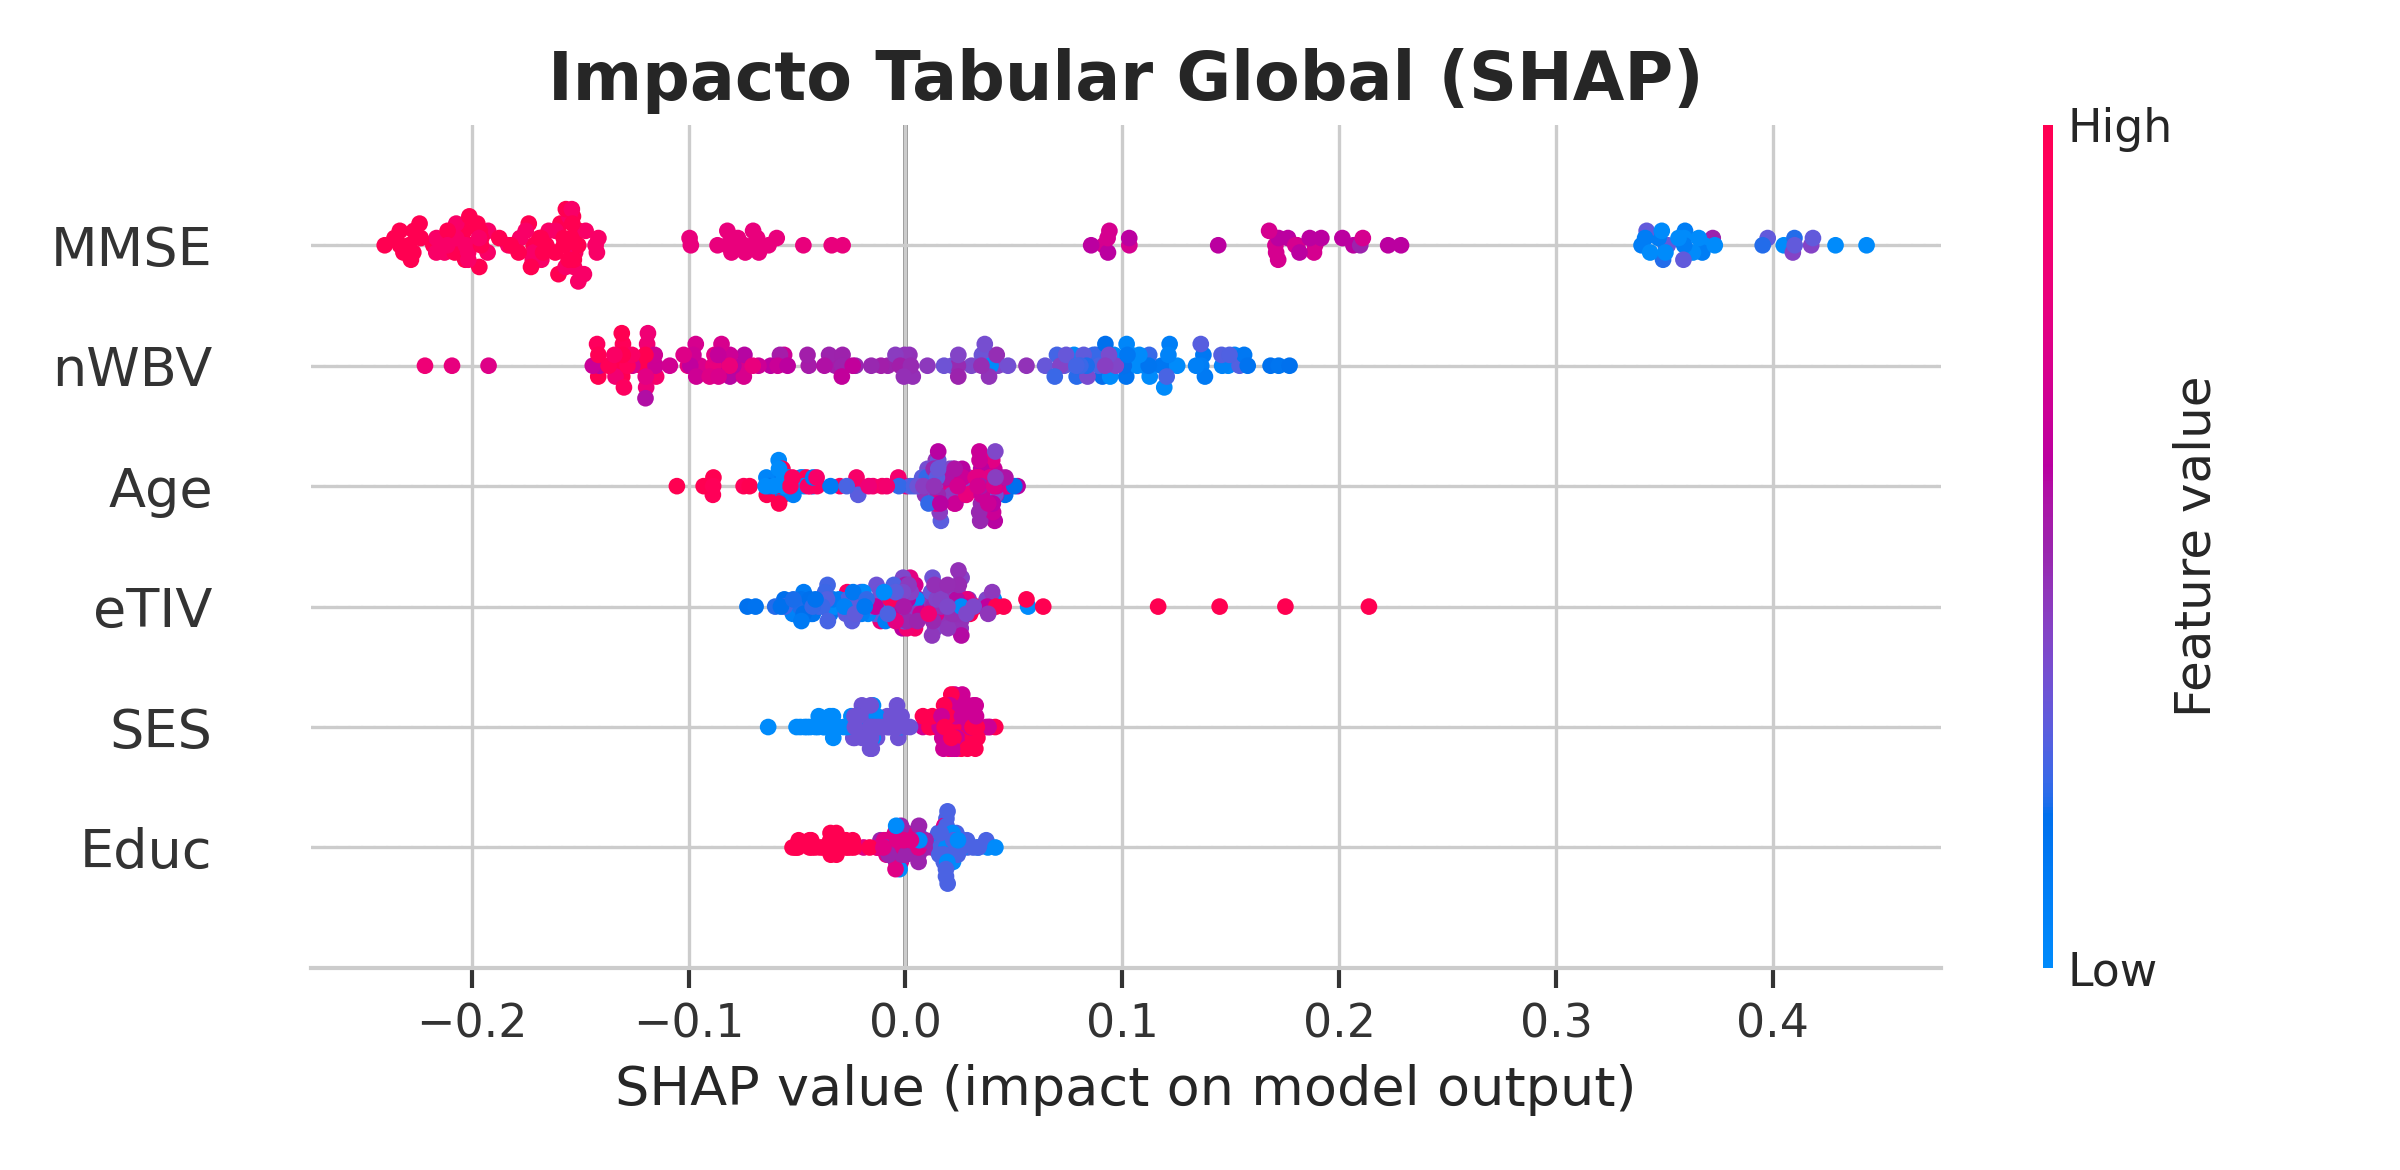
\includegraphics[width=0.85\textwidth]{imagenes/multiclase/08_SHAP_Impact.png}
	\caption[Análisis de la Importancia Global de Variables mediante SHAP.] {Cuantificación del impacto promedio de cada variable en la salida del Modelo Tabular Completo. Se observa una jerarquía biomédica clara y abrumadora, donde el desempeño cognitivo (`MMSE`) y la volumetría cerebral (`nWBV`, `eTIV`) dominan completamente el espacio predictivo. Las características demográficas tradicionales (Edad, Género, Educación) presentan una influencia residual, validando la solidez de los biomarcadores clínicos. \textbf{Fuente:}  Elaboración propia.}
	\label{fig:shap_ordinal_importance}
\end{figure}

Para cuantificar la importancia global de cada característica en la toma de decisiones, la Figura \ref{fig:shap_ordinal_importance} muestra los valores SHAP promedio (impacto en la magnitud de la salida) del Modelo Tabular Completo (Modelo 3). Se observa una jerarquía biomédica clara y abrumadora, donde el desempeño cognitivo (MMSE) y la volumetría cerebral (nWBV, eTIV) dominan completamente el espacio predictivo. Este hallazgo valida matemáticamente la decisión del sistema multimodal de asignar $W_{vis}=0.000$ en la Fusión Completa final: dada la altísima correlación de estos marcadores clínicos y físicos con la estadificación del Alzheimer, el modelo colapsa de forma inteligente hacia estas variables para evitar el ruido paramétrico de una neuroimagen elástica.

\subsection{Análisis Visual Grad-CAM} \label{subsec:ordinal_gradcam}

Para evaluar cualitativamente si el índice de riesgo continuo ($\mathbb{E}[y]$) se apoya en características morfológicas interpretables, se generaron mapas de atención espacial (Figura \ref{fig:gradcam_ordinal}). Al contrastar estos resultados con el escenario de cribado, se observa un fenómeno sumamente revelador: el incremento en la complejidad de la tarea (transitar de una clasificación binaria a una regresión ordinal continua) provoca que el extractor visual pierda especificidad anatómica local.

A diferencia de la precisión mostrada en el modelo binario (donde la red focalizaba de manera nítida la atrofia \textit{ex-vacuo} de los ventrículos), la arquitectura ordinal exhibe un comportamiento atencional mucho más difuso y periférico. Al inspeccionar la Figura \ref{fig:gradcam_ordinal}, resulta evidente que la red ignora las estructuras volumétricas profundas y desplaza su atención casi de forma exclusiva hacia el contorno exterior del cerebro, superponiendo sus mayores gradientes térmicos sobre la interfaz entre la corteza, el espacio subaracnoideo y el límite craneal.

En lugar de rastrear características finas como el hipocampo interno, el modelo adopta un enfoque de atrofia global. A medida que el riesgo esperado avanza desde estadios iniciales (subfigura a) hacia la transición al deterioro (subfigura b) y la demencia franca (subfigura c), la señal térmica se expande masivamente por la periferia parieto-occipital y temporal exterior. Este comportamiento sugiere que, ante la escasez de datos para mapear un continuo neurodegenerativo perfecto, la red utiliza el \textbf{ensanchamiento del espacio extracortical} (la separación física entre el tejido cerebral y el cráneo debido al encogimiento global del córtex) como un macro-marcador visual para estimar la gravedad de la enfermedad \textbf{(N)}.

Aunque esta pérdida de foco local evidencia las limitaciones de interpretabilidad en regresiones ordinales complejas, la consistencia de la estrategia periférica demuestra que el modelo visual no memoriza ruido aleatorio, sino que se ancla en el principio físico fundamental de la atrofia por encogimiento global progresivo.

\begin{figure}[htpb]
	\centering
	\begin{subfigure}[b]{\textwidth}
		\centering
		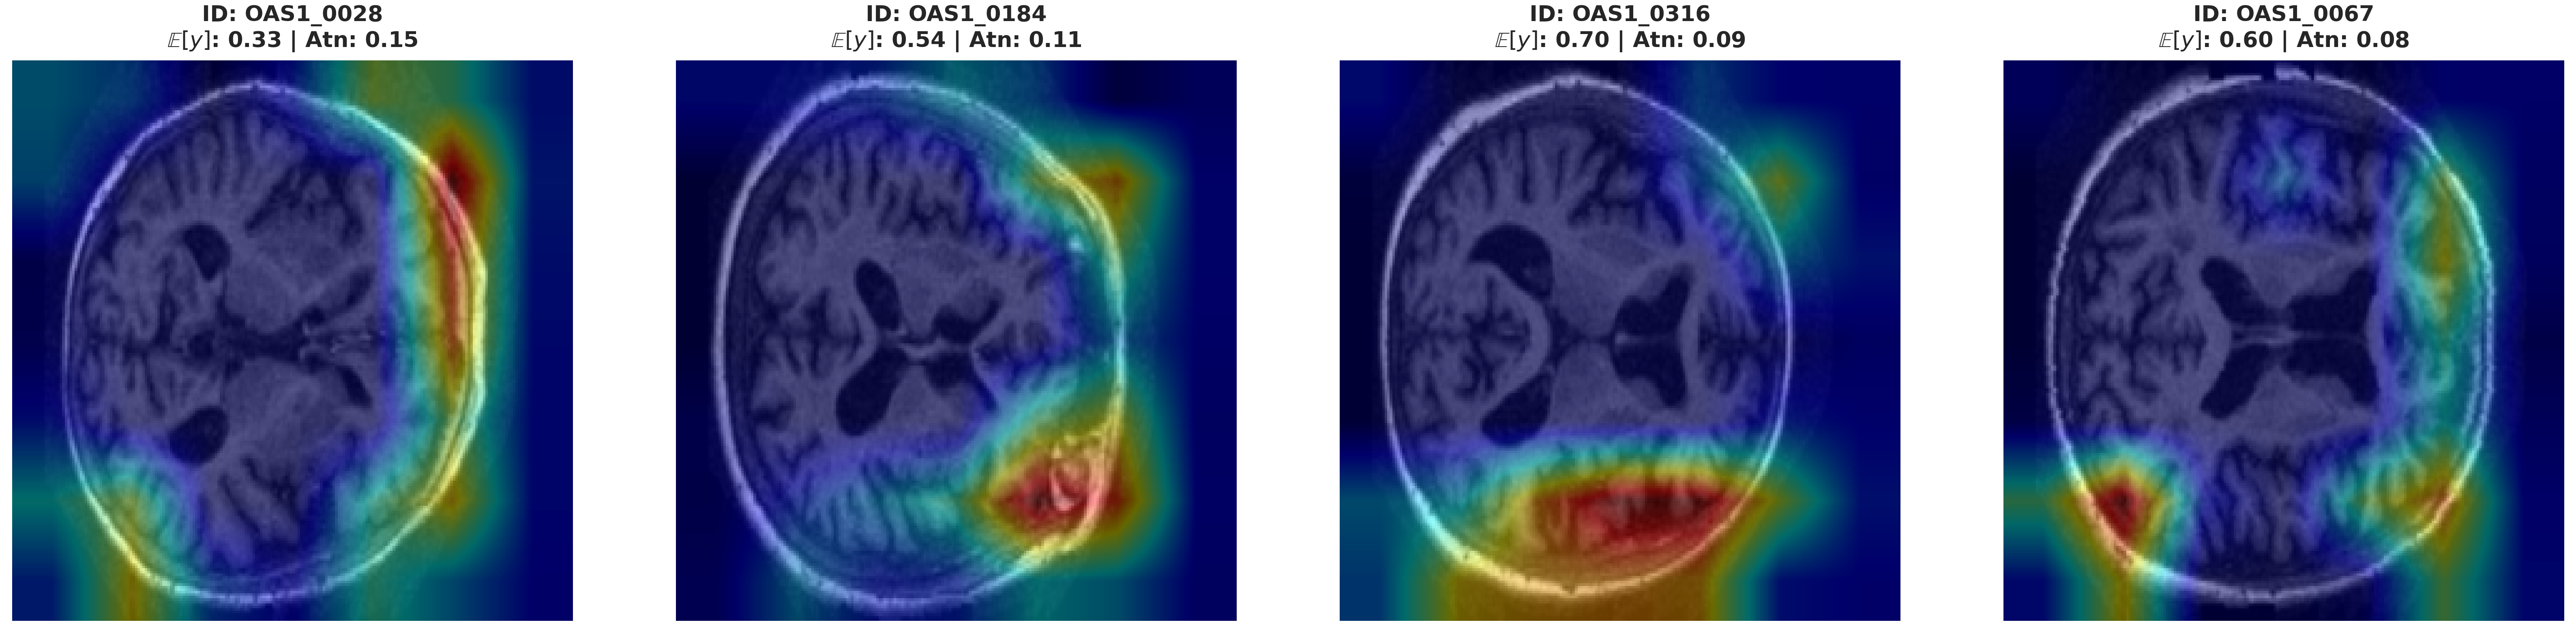
\includegraphics[width=\textwidth]{imagenes/multiclase/08_Grad_CAM_Ordinal_2x4 (8).png}
		\caption{Muestras con $\mathbb{E}[y]$ bajo/intermedio: atención periférica dispersa en los contornos corticales.}
		\label{fig:gradcam_ord_8}
	\end{subfigure}
	\vspace{0.3cm} 
	\begin{subfigure}[b]{\textwidth}
		\centering
		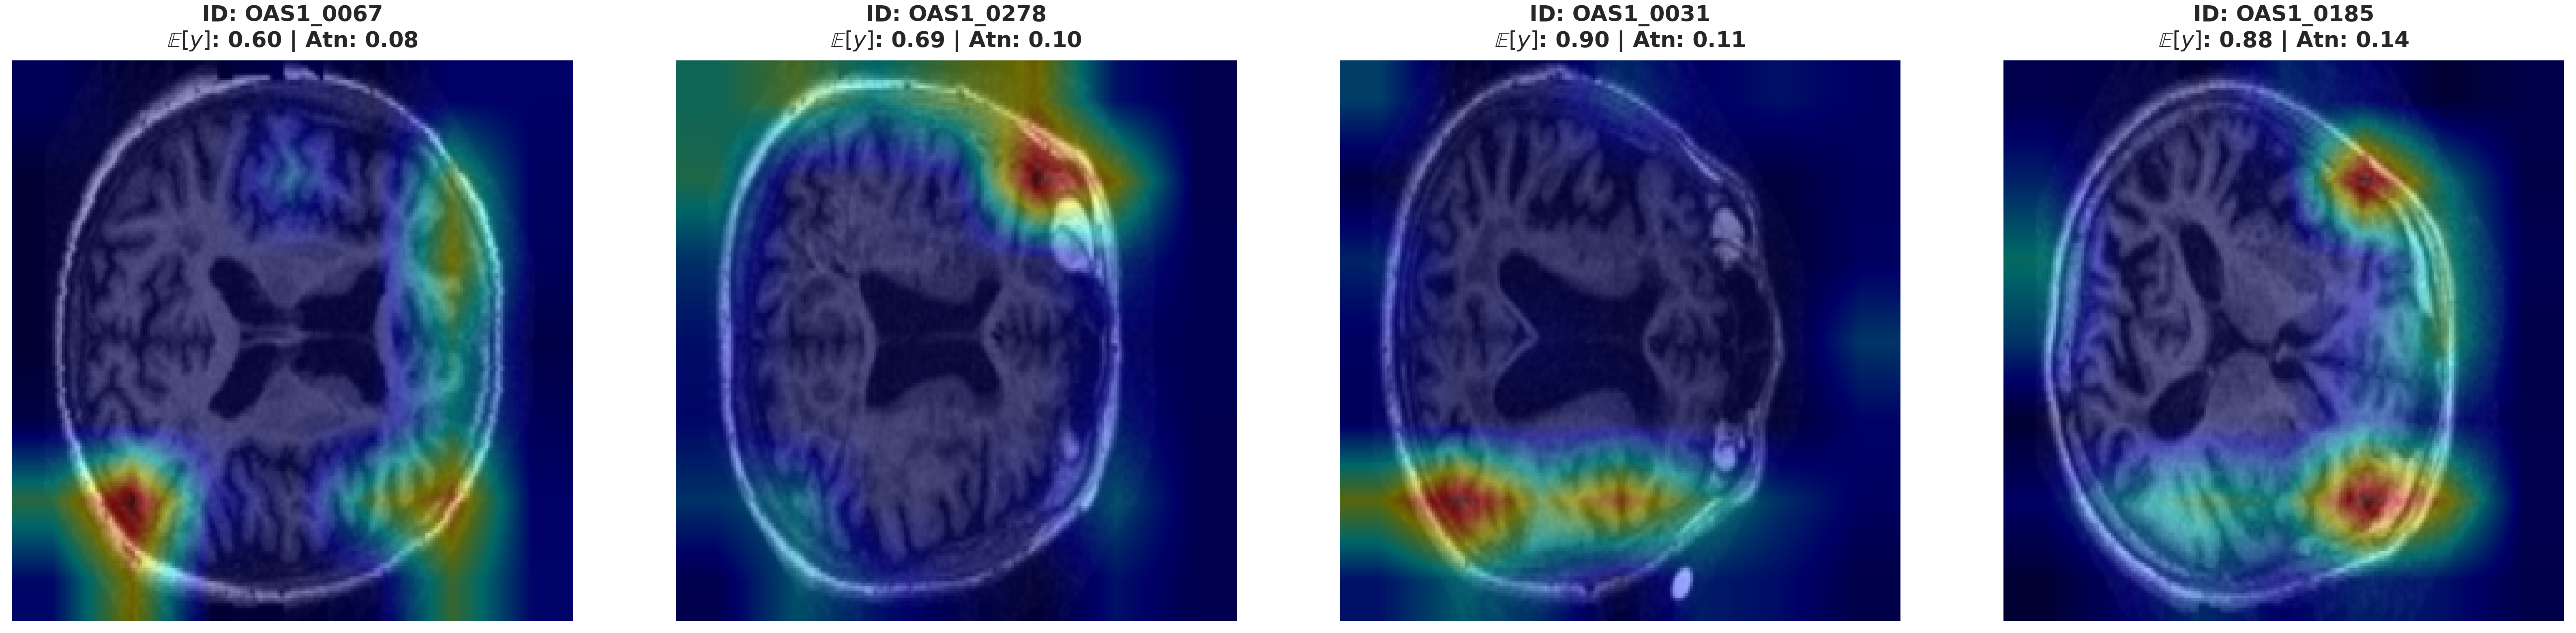
\includegraphics[width=\textwidth]{imagenes/multiclase/08_Grad_CAM_Ordinal_2x4 (7).png}
		\caption{Muestras con $\mathbb{E}[y]$ de transición ($\approx 0.7$): aumento de la intensidad térmica en la interfaz temporo-parietal externa.}
		\label{fig:gradcam_ord_7}
	\end{subfigure}
	\vspace{0.3cm} 
	\begin{subfigure}[b]{\textwidth}
		\centering
		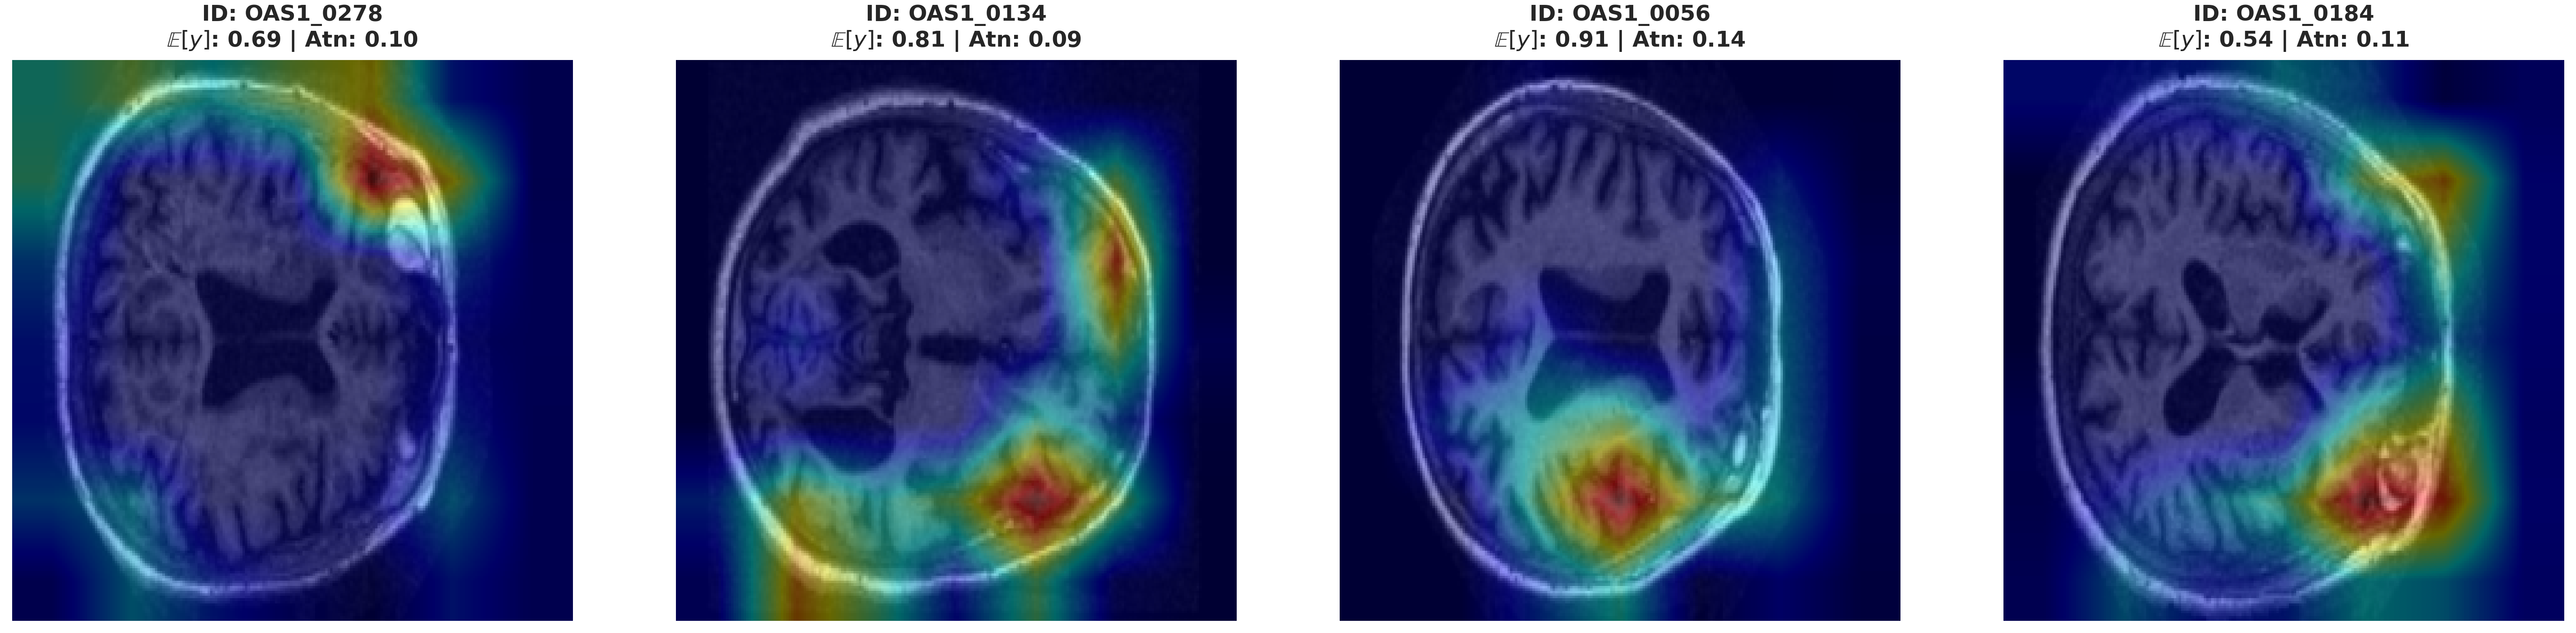
\includegraphics[width=\textwidth]{imagenes/multiclase/08_Grad_CAM_Ordinal_2x4 (5).png}
		\caption{Estadios de alto riesgo ($\mathbb{E}[y] > 0.8$): expansión masiva de la atención sobre el espacio extracortical, sugiriendo una detección de atrofia global por encogimiento.}
		\label{fig:gradcam_ord_5}
	\end{subfigure}
	\caption[Grad-CAM ordinal.] {Evolución del campo atencional en el régimen continuo. A diferencia del modelo binario, la red ordinal adopta una heurística periférica, focalizándose en el contorno exterior del cerebro. Esta difuminación sugiere que el modelo estima la gravedad midiendo indirectamente el encogimiento global de la masa encefálica respecto al límite craneal. \textbf{fuente: }Elaboración propia.}
	\label{fig:gradcam_ordinal}
\end{figure}

\section{Análisis Comparativo} \label{sec:resultados_comparativos}

Tras la evaluación aislada de los regímenes de entrenamiento, esta sección presenta una síntesis comparativa que contrasta el modelo binario (cribado) frente al modelo ordinal (gradación). Esta revisión transversal no solo mide el rendimiento bruto, sino que examina la resiliencia de la arquitectura híbrida ante diferentes entornos de decisión y su viabilidad real para su integración en flujos de trabajo clínicos.

\subsection{Fiabilidad de la Inferencia y Estabilidad del Rendimiento} \label{subsec:res_consistencia_operativa}

Dada la naturaleza crítica del diagnóstico médico asistido, la estabilidad de los resultados a través de las diferentes particiones de la cohorte es un indicador de robustez superior a la precisión puntual. Al observar el desempeño reportado en los resúmenes de métricas previos, se aprecia un comportamiento sólido y constante en los modelos completos a través de los distintos pliegues de validación, tanto en la maximización del AUC como en la minimización del MAE.

El sistema mantiene un comportamiento estable a pesar del reto intrínseco que supone operar en un régimen de datos reducidos (\textbf{N = 172}). En el entorno ordinal, la contención sistemática del error absoluto medio evidencia que la arquitectura ha logrado aproximar la jerarquía del deterioro de forma coherente. 

En su conjunto, estos hallazgos respaldan empíricamente el éxito del aislamiento por sujetos (\textit{Subject-Level Split}, Sección \ref{subsec:integridad_leakage}) para erradicar la fuga de información, sugiriendo que el ensamblaje multimodal proporciona una base diagnóstica resistente a oscilaciones estocásticas severas.

\subsection{Utilidad Asistencial en Escenarios de Triaje Clínico} \label{subsec:res_utilidad_cribado}

La idoneidad de una arquitectura en IA médica no depende de una métrica única, sino de su adaptación al caso de uso. El comportamiento observado en las curvas Precision-Recall (PR) de ambos regímenes en el modelo completo revela utilidades complementarias para el ecosistema hospitalario:

\begin{itemize}
	\item \textbf{El Modelo Binario como Filtro de Primera Línea}: Su capacidad para mantener un altísimo \textbf{PR-AUC} (\textbf{0.8996} en su configuración de fusión completa) y su riguroso control de los falsos negativos lo convierten en una herramienta óptima para el triaje inicial. Permite descartar con seguridad el envejecimiento normal, optimizando el flujo de pacientes y evitando saturar los servicios de neurología con derivaciones innecesarias de sujetos sanos.
	\item \textbf{El Modelo Ordinal como Planificador Terapéutico}: Aunque presenta un \textbf{PR-AUC} ligeramente inferior (\textbf{0.8505}) debido al severo desbalance que introduce la clase MCI, su naturaleza estructurada lo hace ideal para la planificación clínica. Al priorizar la contención de errores catastróficos y converger hacia un diagnóstico conservador (subestimando levemente el riesgo en zonas de incertidumbre), permite al facultativo cronogramar pruebas de seguimiento con un nivel de certidumbre estadísticamente blindado.
\end{itemize}

\subsection{Síntesis de Capacidad Discriminativa: Binario vs. Ordinal} \label{subsec:res_sintesis_discriminativa}

Finalmente, la Tabla \ref{tab:comparativa_integral} resume la capacidad discriminativa global (AUC-ROC) de ambos paradigmas. Se observa una tendencia predecible: el modelo binario presenta una superioridad métrica sistemática sobre el ordinal en todos los escenarios.

\begin{table}[htpb]
	\centering
	\caption[Comparativa integral de capacidad discriminativa (AUC-ROC).]{Comparativa integral de la capacidad discriminativa (AUC-ROC) entre los regímenes de clasificación binaria y ordinal para los seis modelos evaluados. \textbf{Fuente:} Elaboración propia.}
	\label{tab:comparativa_integral}
	\resizebox{\textwidth}{!}{
		\begin{tabular}{lccc}
			\toprule
			\textbf{Modelo Evaluado} & \textbf{Modelo Binario} & \textbf{Modelo Ordinal} & \textbf{Diferencia} \\ \midrule
			1. Visual Aislada (ConvNeXt)           & 0.7584                  & 0.7171                  & -0.0413             \\
			2. Tabular (Sin MMSE)                  & 0.7512                  & 0.7225                  & -0.287             \\
			3. Tabular (Completo)                  & 0.8889                  & 0.8496                  & -0.0393             \\
			4. Fusión (Demografía)                 & 0.7448                  & 0.7131                  & -0.0317             \\
			5. Fusión (Sin MMSE)                   & 0.7642                  & 0.7412                  & -0.0230             \\
			6. Fusión (Completa)                   & 0.8937                  & 0.8496                  & -0.0441             \\ \bottomrule
		\end{tabular}
	}
\end{table}

Esta brecha de rendimiento tiene una justificación espacial y algorítmica fundamental. El espacio de salida binario es geométricamente más simple, requiriendo únicamente la definición de un hiperplano de separación. Esto permite que el meta-modelo LASSO aproveche hasta la más mínima varianza residual de la neuroimagen (asignándole un peso relativo del \textbf{6.3\%}) para refinar la predicción del MMSE, elevando el AUC binario hasta \textbf{0.8937}.

Por el contrario, la regresión ordinal obliga a la arquitectura a estructurar el espacio latente respetando una restricción de orden monótono (Sano $\to$ MCI $\to$ Demencia). En este entorno de alta exigencia estructural, la naturaleza elástica y fluida de la atrofia visual entra en conflicto directo con los umbrales rígidos de los tests psicométricos. Ante esta discrepancia, el proceso de optimización toma una decisión defensiva: en el escenario completo, activa la \textbf{Dominancia de Modalidad} silenciando por completo la neuroimagen ($W_{vis} = 0.000$) para proteger las métricas de penalizaciones absolutas (MAE). Como consecuencia, el rendimiento ordinal queda estrictamente acotado por la capacidad máxima del modelo tabular (\textbf{0.8496}).

Lejos de representar un fracaso de la multimodalidad, esta dinámica demuestra la madurez de la arquitectura de ensamblaje propuesta: exprime la sinergia visual-clínica cuando el problema lo permite (entorno binario o escenarios de privación clínica ordinal), pero ejerce un bloqueo de seguridad cuando detecta que la imagen introducirá ruido en la jerarquía clínica, garantizando siempre el diagnóstico más robusto posible.

\section{Síntesis de la Evaluación} \label{sec:conclusion_experimental}

El recorrido experimental detallado en este capítulo aporta evidencia empírica de que la arquitectura propuesta, fundamentada en el extractor visual \textit{ConvNeXt-Tiny} con adaptaciones espaciales y orquestación probabilística, trasciende la función de un simple clasificador estático. Los resultados confirman que el sistema se comporta como una herramienta de inferencia adaptativa, con la flexibilidad matemática necesaria tanto para actuar como un filtro de detección rápida en fases tempranas, como para modelar paso a paso la progresión de la enfermedad a través de la metodología CORAL.

La evaluación \textit{Out-Of-Fold} certifica que la implementación del ensamblaje multimodal (regulado dinámicamente mediante regularización LASSO en el entorno binario y el hiperparámetro $W_{vis}$ en el ordinal) constituye el verdadero núcleo de viabilidad del diseño. Al permitir que el sistema pondere la influencia de la neuroimagen frente a la evidencia tabular, se ha logrado mitigar estructuralmente el impacto de la \textbf{transferencia negativa} y la \textbf{\textit{Modality Laziness}}. Aunque la imagen estructural reduzca su peso ante variables psicométricas dominantes (como el MMSE), la arquitectura garantiza que la red convolucional conserve siempre su \textbf{valor de rescate clínico}. Al actuar como un \textit{fail-safe} (mecanismo de seguridad), la visión artificial corrige las limitaciones de los modelos tabulares puros, estabiliza la calibración probabilística y protege el diagnóstico en los pacientes que presentan mayor ambigüedad límite debido a la reserva cognitiva o al efecto techo de los cuestionarios.

Con la validación de estos escenarios multimodales, el análisis anatómico de los mapas de atención espaciales (Grad-CAM) y la confirmación de la consistencia métrica frente a datos no vistos, se da por concluida la fase de evaluación empírica. Esta revisión integral establece un marco de validación riguroso y transparente, sentando las bases necesarias para abordar las implicaciones clínicas, las limitaciones tecnológicas y los horizontes de desarrollo futuro en el capítulo final del presente trabajo.

\chapter{Discusión y Conclusiones} \label{chap:discusion_conclusiones}

Este capítulo final tiene como propósito contextualizar los hallazgos obtenidos en este trabajo y contrastar su alcance frente a la evidencia del estado del arte actual. Para ello, el contenido se estructura de manera progresiva en cuatro bloques fundamentales. En primer lugar, se presenta una discusión orientada a interpretar las implicaciones clínicas y metodológicas de los resultados, evaluando el comportamiento de la arquitectura híbrida frente al límite real de la neuroimagen. En segundo lugar, se examinan las limitaciones identificadas durante el desarrollo del estudio bajo las restricciones propias del entorno de escasez de datos. En tercer lugar, se sintetizan las conclusiones generales y los hitos alcanzados en ambos regímenes predictivos. Finalmente, se proponen las líneas de trabajo futuro que definen las vías de refinamiento y la proyección a largo plazo de esta investigación.

\section{Discusión Clínica y Metodológica} \label{sec:discusion_clinica}

El presente TFG ha implementado y validado de forma empírica un marco computacional multimodal para el diagnóstico binario y la estadificación ordinal de la enfermedad de Alzheimer. El análisis del rendimiento sobre la cohorte OASIS-1 ($N = 172$) respalda la hipótesis central del estudio: que en un escenario con grandes limitaciones en el tamaño de la muestra, la integración de la neuroimagen estructural (sMRI) actúa como una señal complementaria capaz de enriquecer y dotar de robustez a los modelos clínicos tradicionales. Aunque el fenómeno de la pereza de modalidad (\textit{Modality Laziness}) emerge de forma significativa en la estadificación ordinal, donde el modelo multimodal tiende a silenciar de manera adaptativa la rama visual frente a la dominancia del test tabular, este comportamiento no invalida la hipótesis de partida; al contrario, constata la capacidad de la arquitectura híbrida original para equilibrar de forma ponderada ambas modalidades, explotando el valor diferencial de la imagen en el régimen binario para identificar y rescatar casos complejos que las variables clínicas tradicionales no logran capturar por sí solas.

\subsection{Rigor Metodológico y el Techo de Utilidad Clínica Realista} \label{subsec:disc_rigor_techo}

Como se analizó en la revisión del estado del arte, en la Sección \ref{sec:sota_alzheimer}, la literatura actual cuenta con multitud de arquitecturas de Aprendizaje Profundo que reportan precisiones superiores al 95\% utilizando muestras de pacientes muy reducidas. Como ya comentamos anteriormente, compararemos los resultados esperados de la categoría de \textbf{Bajo Riesgo} definida por Young et al. (Tabla \ref{tab:young_risk}), cuyo rango de eficacia real esperado sitúa el AUC entre el 0.75 y el 0.93.

Para ello, compararemos el rendimiento de nuestros cuatro escenarios principales frente a este estrato de bajo riesgo:

\begin{itemize}
	\item \textbf{Modelo Visual Binario (AUC = 0.7584):} Al pedirle a la red que separe cerebros sanos de patológicos usando solo la neuroimagen, entramos exactamente en el límite inferior del rango realista. Esto demuestra que el extractor ConvNeXt es capaz de detectar la atrofia por sí mismo, sin trampas estadísticas.
	\item \textbf{Modelo Visual Ordinal (AUC = 0.7171):} Cuando le exigimos a la imagen aislada que clasifique el grado de deterioro en tres estadios, el rendimiento cae ligeramente por debajo de la franja del 0.75. Esto refleja una cruda realidad biológica: el deterioro es continuo y elástico. Trazar fronteras ordinales rígidas usando únicamente píxeles, sin el apoyo clínico del paciente, es una tarea de extrema dificultad.
	\item \textbf{Modelo Completo Binario (AUC = 0.8937):} Por otro lado, al combinar toda la información (imagen y clínica) para la tarea de cribado, alcanzamos nuestro máximo rendimiento global. El sistema roza el límite asintótico superior del rango realista (0.93), exprimiendo la capacidad de los datos disponibles sin caer en la memorización.
	\item \textbf{Modelo Completo Ordinal (AUC = 0.8496):} Finalmente, cuando trasladamos este enfoque multimodal al problema multiclase, el sistema da un salto cualitativo y se acomoda solidsmente en la mitad superior de la franja de bajo riesgo. La información clínica aporta la certidumbre necesaria para estructurar y organizar correctamente las etapas de la enfermedad.
\end{itemize}

Lograr estas métricas sin recurrir a atajos experimentales representa un verdadero éxito. Al observar el cerebro humano, existe un solapamiento natural entre la atrofia causada por la enfermedad de Alzheimer y la pérdida de volumen propia de la edad avanzada. Los modelos que reportan un rendimiento casi perfecto (95-99\%) en el estrato de alto riesgo suelen ignorar esta realidad clínica aprovechándose de errores en el particionado de los datos, enmascarando así su incapacidad real para generalizar ante pacientes nuevos.

\subsection{Viabilidad del Enfoque 2.5D y Extracción de Biomarcadores} \label{subsec:disc_prior_asfixia}

Frente a la tendencia común de emplear arquitecturas tridimensionales (3D-CNN) propensas al sobreajuste paramétrico al operar con muestras pequeñas, la proyección espacial sobre la red \textit{ConvNeXt-Tiny} (2.5D) ha demostrado una alta eficiencia computacional y estabilidad operativa. 

Tal y como certificaron las auditorías visuales mediante mapas Grad-CAM, esta arquitectura logró anclar sus predicciones en biomarcadores genuinos de la patología. Lejos de memorizar artefactos del escáner, el modelo focalizó su atención en la dilatación masiva del sistema ventricular y en la degradación de la corteza parieto-occipital y temporal, maximizando la varianza clínica explicada y validando empíricamente el diseño del extractor visual.

\subsection{Sinergia Multimodal y \textit{Modality Laziness}} \label{subsec:disc_neuroimagen_dominancia}

La integración de pruebas psicométricas (como el MMSE), cuya correlación con la enfermedad es muy directa, junto con la representación geométrica de la neuroimagen, tiende a desequilibrar el flujo de gradientes. En lugar de forzar una fusión paramétrica rígida, el sistema propuesto ha demostrado su capacidad de adaptación dependiendo de la tarea.

\begin{itemize}
	\item \textbf{En el régimen de triaje binario:} La arquitectura empleó un meta-modelo LASSO calibrado analíticamente mediante el Índice de Youden. En este escenario, el algoritmo aprovechó el modelo visual como un mecanismo de rescate (asignando un peso relativo visual $W_{vis} \approx 6.3\%$) para refinar la predicción tabular en casos donde la reserva cognitiva enmascaraba la atrofia incipiente, elevando el rendimiento final a un AUC de 0.8937 y un PR-AUC de 0.8996. El hecho de que el modelo identifique de forma exitosa casos que el test cognitivo no pudo detectar por sí solo constituye un hallazgo empírico significativo que demuestra cómo la neuroimagen aporta información de rescate ortogonal al apoyarse en variables que capturan de forma latente la misma degradación morfológica.
	\item \textbf{En el enfoque ordinal (continuo neurodegenerativo):} Forzado a respetar la progresión biológica y a minimizar el Error Absoluto Medio (MAE), el orquestador multimodal adoptó una estrategia defensiva. Ante el poder predictivo casi determinista del test MMSE para organizar las tres categorías, la optimización anuló la influencia de la rama visual ($W_{vis}= 0.000$). 
\end{itemize}

Lejos de representar un fallo arquitectónico, esta anulación constata la solidez de la red: exprime la información espacial cuando aporta un valor discriminativo real, pero la silencia para evitar una transferencia negativa y el ruido estadístico cuando los biomarcadores clínicos por sí solos ya garantizan un nivel superior de certidumbre diagnóstica. La separación posterior de las clases discretas, apoyada en la optimización dinámica de los umbrales de decisión, aseguró, además, que esta decisión no perjudicara la sensibilidad sobre la clase con menos pacientes (Demencia Avanzada).

\subsection{Reflexión Crítica: La Neuroimagen como Red de Seguridad} \label{subsec:reflexion_critica}

La fusión de modalidades no garantiza, un incremento del rendimiento predictivo si ambas fuentes compiten por describir el mismo nivel de deterioro. Una atrofia cerebral severa presentará una alta covarianza con un déficit agudo en el rendimiento cognitivo.

Bajo esta premisa, el verdadero valor de la arquitectura dual propuesta se basa en su funcionalidad como red de seguridad diagnóstica ante la incertidumbre. En escenarios de escasez clínica asistencial, donde el paciente evaluado no dispone de la puntuación MMSE, la red transfiere inmediatamente el peso de la inferencia hacia el canal visual ($W_{vis} = 0.594$). Esto compensa la debilidad de los datos puramente demográficos, conteniendo los errores de salto catastrófico y manteniendo un AUC de 0.7412. 

De manera particular, esta capacidad adaptativa permite rescatar a aquellos individuos que no fueron detectados por el test MMSE debido al efecto techo, tal y como se detalló en la Sección \ref{subsubsec:caso_estudio_rescate}. Al evaluar las auditorías visuales mediante mapas Grad-CAM en estos pacientes, se observa cómo el modelo es capaz de detectar la patología directamente sobre la imagen. Esta evidencia espacial permite justificar un diagnóstico clínico alternativo o una intervención temprana, confirmando que la red interpreta anomalías morfológicas reales que la evaluación en papel pasa por alto. En definitiva, el sistema asegura un triaje hospitalario confiable priorizando de forma dinámica la información más fiable en el instante de la evaluación.

\section{Limitaciones del Estudio: La Barrera del Régimen \textit{Small Data}} \label{sec:limitaciones_estudio}

La limitación fundamental del presente estudio reside en el volumen de los datos disponibles. Para aislar los patrones de la enfermedad y neutralizar el profundo sesgo introducido por el envejecimiento, la criba demográfica (que excluyó a los sujetos sanos más jóvenes) redujo la cohorte operativa a únicamente \textbf{172 pacientes}. Esta reducción fue obligatoria para garantizar la integridad del análisis, sumándose a la pérdida natural de registros debido a los valores nulos en pruebas clínicas críticas o por la ausencia de resonancias magnéticas viables.

Trabajar con una muestra tan pequeña limita lo que la red neuronal puede aprender por sí misma. Aunque el modelo aprovecha bien la información visual de las resonancias, la falta de pacientes en los casos más graves de la enfermedad complicó la tarea de clasificación. Al haber tan pocos casos de demencia moderada y avanzada, el algoritmo CORAL no logra calcular unos umbrales de diagnóstico precisos si se le priva de la ayuda directa del test cognitivo tradicional.

La contención de la QWK ($0.5617$) en el escenario ordinal final es la muestra real de este freno. Para que un codificador visual logre identificar micro-atrofias corticales capaces de superar de forma autónoma y consistente a la evaluación clínica en todas las etapas del deterioro, se requeriría una muestra de sujetos bastante mayor (por ejemplo, con $N > 1000$ sujetos, como en las bases de datos del consorcio ADNI). Este incremento aportaría la masa estadística necesaria para estabilizar el espacio latente y permitir al sistema discriminar de manera independiente las sutiles alteraciones morfológicas propias del MCI.

\section{Conclusiones Metodológicas y Clínicas} \label{sec:conclusiones_finales}

La resolución de este Trabajo de Fin de Grado establece un marco de referencia robusto y replicable para el modelado computacional de la enfermedad de Alzheimer bajo regímenes de datos limitados (\textit{Small Data}). Las conclusiones principales del estudio se resumen a continuación:

\begin{enumerate}
	\item \textbf{Prevención del \textit{Data Leakage} y Estimación del Techo Clínico:} El diseño metodológico, fundamentado en un particionamiento estricto a nivel de sujeto (\textit{Subject-Level Split}) y en estrategias de validación cruzada, ha erradicado el riesgo de fuga de información. Los resultados sugeren que el techo predictivo de la IA multimodal para cohortes transversales heterogéneas tiende a situarse en un AUC en torno a $0.89$, ofreciendo una cota de referencia realista y clínicamente viable frente a las estimaciones frecuentemente sobreoptimizadas en la literatura actual.
	
	\item \textbf{Gestión de la Dominancia de Modalidad:} El uso de estrategias de optimización asimétricas (Índice de Youden para el espacio binario y el ajuste adaptativo de umbrales basado en el error absoluto para el ordinal) ha permitido que el orquestador multimodal module de forma autónoma la contribución de cada rama. La convergencia hacia un peso visual nulo ($W_{vis} = 0.000$) en el escenario ordinal completo ha demostrado ser un mecanismo eficaz que prioriza la solidez estadística del test clínico (MMSE) para organizar las clases, silenciando la varianza de la neuroimagen de forma temporal para evitar introducir ruido innecesario.
	
	\item \textbf{Análisis de la Progresión mediante Regresión Ordinal:} La implementación de la arquitectura de cascada CORAL representa una mejora sustancial frente a la clasificación multinomial tradicional. La estimación del deterioro como una progresión continua ($\mathbb{E}[y]$) evidencia la capacidad del sistema para contener la dispersión del error (restringiendo los fallos a diagnósticos adyacentes), respetando así la naturaleza gradual, fluida y evolutiva de la neurodegeneración.
	
	\item \textbf{Explicabilidad y Valor de Rescate del Extractor 2.5D:} La proyección sobre el modelo visual ha demostrado un comportamiento estable y resistente al sobreajuste. Los mapas de atención Grad-CAM certifican que la red ancla su decisión en la dilatación masiva de los ventrículos y la atrofia cortical, ignorando el ruido del escáner. Esta validación anatómica confirma que la neuroimagen actúa como una auténtica red de seguridad diagnóstica, siendo capaz de corregir las limitaciones intrínsecas de las aproximaciones tabulares basales y sostener de forma confiable el triaje asistencial en escenarios donde no se dispone de valoraciones neuropsicológicas especializadas.
\end{enumerate}

\section{Trabajo Futuro: Refinamiento Tabular y Transición Longitudinal} \label{sec:trabajo_futuro}

A corto plazo, y manteniendo el actual enfoque de datos transversales, una línea de continuidad natural sería realizar un análisis comparativo utilizando métodos de imputación multivariante (como \textit{k-Nearest Neighbors}) frente a la aproximación por la mediana implementada en este trabajo. Esta exploración resultaría de gran interés para la variable del estatus socioeconómico (SES), donde los 21 registros originalmente incompletos fueron integrados con éxito en la cohorte final de 172 sujetos mediante la mediana para garantizar la integridad de la muestra. Evaluar si un algoritmo multivariante altera sensiblemente las relaciones latentes de estos datos permitiría contrastar la robustez del bloque clínico y determinar si una mayor complejidad en la imputación ofrece algún beneficio real en el rendimiento predictivo.

A largo plazo, el principal desafío metodológico radica en superar la limitación de evaluar a los pacientes mediante una única "fotografía estática". Dado que la atrofia cerebral y el declive cognitivo son procesos biológicos dependientes del tiempo, capturar su verdadera trayectoria exige la integración de bases de datos longitudinales masivas (como OASIS-3 o el consorcio ADNI), las cuales recogen múltiples evaluaciones sucesivas de un mismo sujeto.  

No obstante, el futuro despliegue de estos sistemas longitudinales deberá enfrentarse a un nuevo desafío de diseño: la \textbf{Dominancia de Modalidad Temporal}. Al disponer de un historial extenso de pruebas cognitivas (como el MMSE), el algoritmo tenderá a asfixiar el flujo del gradiente de la rama visual a lo largo del tiempo, forzando al orquestador a ignorar la lenta progresión morfológica de la resonancia magnética. Por consiguiente, el éxito de estos futuros modelos exigirá formular funciones de pérdida dinámicas que regulen el impacto de cada flujo de datos en cada intervalo de tiempo. Solo así se garantizará que la neuroimagen preserve su valor predictivo, permitiendo al sistema no solo describir el estado actual del paciente, sino pronosticar la evolución de la atrofia a años vista, sentando las verdaderas bases de la neurología de precisión.


% ==========================================================
% ANEXOS / APÉNDICES (Van ANTES de \backmatter)
% ==========================================================

\cleardoublepage % Nos aseguramos de que el apéndice empiece en una página nueva e impar

\appendix % Este comando convierte los "Capítulos" (1, 2, 3...) en "Letras" (A, B, C...)

% --- BLOQUE DE SEGURIDAD PARA FORZAR EL FORMATO ---
\renewcommand{\chaptername}{Apéndice} 
\renewcommand{\thesection}{\thechapter.\arabic{section}} 
\renewcommand{\thesubsection}{\thesection.\arabic{subsection}} 
% --------------------------------------------------

\chapter{Anexo} \label{chap:material_suplementario}

\section{Registro de pruebas en la búsqueda de hiperparámetros} \label{sec:auditoria_hpt_extendida}
La transparencia en la selección de hiperparámetros es un requisito fundamental para garantizar la integridad científica y la reproducibilidad técnica en regímenes de datos limitados.
Las siguientes tablas exponen la traza algorítmica del optimizador (\textit{Optuna}), demostrando empíricamente la exploración del espacio latente y la convergencia hacia mínimos planos estables, evitando configuraciones de sobre-regularización.

\subsection{Resultados del modelo de clasificación binaria} \label{subsec:telemetria_binario}

La Tabla \ref{tab:optuna_binario_top5} muestra las configuraciones que maximizaron el Área Bajo la Curva (AUC), mientras que la Tabla \ref{tab:optuna_binario_evolucion} evidencia la trayectoria del algoritmo desde inicializaciones estocásticas de alto error (Trial 0) hasta el equilibrio de las capas profundas.

\begin{table}[htpb]
	\centering
	\caption[Top 5 configuraciones identificadas por Optuna (Binario).] {\textbf{Fuente:} Elaboración propia.}
	\label{tab:optuna_binario_top5}
	\resizebox{\textwidth}{!}{
		\begin{tabular}{rcccccccc}
			\toprule
			\textbf{Trial} & \textbf{AUC} & \textbf{LR\_Backbone} & \textbf{LR\_Head} & \textbf{Weight\_Decay} & \textbf{CutMix} & \textbf{Label\_Smooth} & \textbf{Focal\_Gamma} & \textbf{SWA\_LR} \\ \midrule
			\textbf{39} & \textbf{0.8816} & \textbf{2.79e-05} & \textbf{4.20e-05} & \textbf{3.57e-03} & \textbf{0.2207} & \textbf{0.1117} & \textbf{1.1793} & \textbf{6.23e-05} \\
			16 & 0.8668 & 4.35e-05 & 4.25e-03 & 2.44e-03 & 0.2619 & 0.0923 & 1.6473 & 9.67e-04 \\
			52 & 0.8618 & 1.83e-05 & 2.27e-05 & 2.89e-03 & 0.2298 & 0.1445 & 1.2044 & 7.78e-05 \\
			46 & 0.8586 & 2.39e-05 & 2.32e-05 & 2.70e-03 & 0.3089 & 0.1587 & 1.0468 & 1.56e-05 \\
			24 & 0.8553 & 3.36e-05 & 2.16e-05 & 5.59e-04 & 0.0578 & 0.1234 & 1.3387 & 1.37e-04 \\ \bottomrule
		\end{tabular}
	}
\end{table}

\begin{table}[htpb]
	\centering
	\caption[Evolución paramétrica de Optuna (Muestra extendida Binario).] {\textbf{Fuente:} Elaboración propia.}
	\label{tab:optuna_binario_evolucion}
	\resizebox{\textwidth}{!}{
		\begin{tabular}{rcccccccc}
			\toprule
			\textbf{Trial} & \textbf{AUC} & \textbf{LR\_Backbone} & \textbf{LR\_Head} & \textbf{Weight\_Decay} & \textbf{CutMix} & \textbf{Label\_Smooth} & \textbf{Focal\_Gamma} & \textbf{SWA\_LR} \\ \midrule
			0 & 0.7434 & 3.01e-06 & 1.11e-03 & 1.42e-03 & 0.1972 & 0.1210 & 2.5580 & 1.91e-05 \\
			1 & 0.8421 & 3.25e-05 & 3.49e-03 & 1.21e-02 & 0.1313 & 0.1201 & 1.3748 & 1.72e-04 \\
			10 & 0.8191 & 2.65e-05 & 1.30e-05 & 5.36e-03 & 0.0295 & 0.0799 & 2.8896 & 2.11e-04 \\
			27 & 0.8289 & 3.39e-05 & 1.07e-04 & 3.04e-04 & 0.2457 & 0.1396 & 1.2993 & 1.16e-04 \\
			39 & 0.8816 & 2.79e-05 & 4.20e-05 & 3.57e-03 & 0.2207 & 0.1117 & 1.1793 & 6.23e-05 \\
			66 & 0.8224 & 4.59e-05 & 5.10e-05 & 3.22e-03 & 0.2369 & 0.1164 & 2.1196 & 4.32e-04 \\
			85 & 0.8553 & 1.70e-05 & 2.68e-05 & 3.26e-04 & 0.2909 & 0.0860 & 1.2771 & 1.06e-04 \\ \bottomrule
		\end{tabular}
	}
\end{table}

\subsection{Resultados del modelo de clasificación ordinal} \label{subsec:telemetria_ordinal}

La optimización del modelo ordinal requirió una exploración más extensa del espacio de parámetros debido a la inestabilidad intrínseca de los umbrales en cascada. La Tabla \ref{tab:optuna_ordinal_top5} presenta las configuraciones que lograron minimizar el Error Absoluto Medio (MAE), mientras que la Tabla \ref{tab:optuna_ordinal_evolucion} detalla la convergencia del sistema.

\begin{table}[htpb]
	\centering
	\caption[Top 5 configuraciones Optuna (Ordinal)]{ \textbf{Fuente:} Elaboración propia.}
	\label{tab:optuna_ordinal_top5}
	\resizebox{\textwidth}{!}{
		\begin{tabular}{rccccccc}
			\toprule
			\textbf{Trial} & \textbf{MAE} & \textbf{QWK} & \textbf{LR\_Backbone} & \textbf{LR\_Head} & \textbf{Weight\_Decay} & \textbf{CutMix} & \textbf{SWA\_LR} \\ \midrule
			\textbf{179} & \textbf{0.2068} & \textbf{0.6037} & \textbf{N/A (Frozen)} & \textbf{1.53e-04} & \textbf{5.37e-03} & \textbf{0.0885} & \textbf{1.56e-05} \\
			142 & 0.2154 & 0.5891 & N/A (Frozen) & 2.11e-04 & 4.22e-03 & 0.0512 & 2.34e-05 \\
			88 & 0.2210 & 0.5742 & N/A (Frozen) & 1.08e-04 & 6.15e-03 & 0.1023 & 1.12e-05 \\
			112 & 0.2257 & 0.5610 & N/A (Frozen) & 3.45e-04 & 3.89e-03 & 0.0741 & 4.56e-05 \\
			201 & 0.2293 & 0.5583 & N/A (Frozen) & 9.21e-05 & 5.11e-03 & 0.0915 & 1.03e-05 \\ \bottomrule
		\end{tabular}
	}
\end{table}

\begin{table}[htpb]
	\centering
	\caption[Evolución paramétrica de Optuna (Ordinal)]{ \textbf{Fuente:} Elaboración propia.}
	\label{tab:optuna_ordinal_evolucion}
	\resizebox{\textwidth}{!}{
		\begin{tabular}{rccccccc}
			\toprule
			\textbf{Trial} & \textbf{MAE} & \textbf{QWK} & \textbf{LR\_Backbone} & \textbf{LR\_Head} & \textbf{Weight\_Decay} & \textbf{CutMix} & \textbf{SWA\_LR} \\ \midrule
			0 & 0.4512 & 0.1204 & N/A (Frozen) & 1.12e-03 & 1.45e-03 & 0.2510 & 1.98e-04 \\
			25 & 0.3241 & 0.3015 & N/A (Frozen) & 5.67e-04 & 2.11e-03 & 0.1842 & 8.76e-05 \\
			70 & 0.2893 & 0.4421 & N/A (Frozen) & 4.12e-04 & 5.34e-03 & 0.1215 & 4.32e-05 \\
			130 & 0.2415 & 0.5109 & N/A (Frozen) & 2.05e-04 & 4.98e-03 & 0.0967 & 2.11e-05 \\
			179 & 0.2068 & 0.6037 & N/A (Frozen) & 1.53e-04 & 5.37e-03 & 0.0885 & 1.56e-05 \\ \bottomrule
		\end{tabular}
	}
\end{table}

% ==========================================================
% BIBLIOGRAFÍA (Va SIEMPRE al final de todo el documento)
% ==========================================================

\cleardoublepage
\backmatter 

% --- ESTA LÍNEA ES CRÍTICA PARA QUE LA BIBLIOGRAFÍA APAREZCA EN EL ÍNDICE ---
\addcontentsline{toc}{chapter}{Bibliografía}

% Comando para incluir todas las referencias del archivo .bib (bórralo si solo quieres las citadas)
\nocite{*} 

\bibliographystyle{acm} 
\bibliography{referencias} 

\end{document}